\documentclass[journal,12pt,twocolumn]{IEEEtran}
%
\usepackage{setspace}
\usepackage{gensymb}
%\doublespacing
\singlespacing

%\usepackage{graphicx}
%\usepackage{amssymb}
%\usepackage{relsize}
\usepackage[cmex10]{amsmath}
%\usepackage{amsthm}
%\interdisplaylinepenalty=2500
%\savesymbol{iint}
%\usepackage{txfonts}
%\restoresymbol{TXF}{iint}
%\usepackage{wasysym}
\usepackage{amsthm}
\usepackage{iithtlc}
\usepackage{mathrsfs}
\usepackage{txfonts}
\usepackage{stfloats}
\usepackage{cite}
\usepackage{cases}
\usepackage{subfig}
%\usepackage{xtab}
\usepackage{longtable}
\usepackage{multirow}
%\usepackage{algorithm}
%\usepackage{algpseudocode}
\usepackage{enumitem}
\usepackage{mathtools}
\usepackage{tikz}
\usepackage{circuitikz}
\usepackage{verbatim}
\usepackage{hyperref}
%\usepackage{stmaryrd}
\usepackage{tkz-euclide} % loads  TikZ and tkz-base
\usetkzobj{all}
\usepackage{listings}
    \usepackage{color}                                            %%
    \usepackage{array}                                            %%
    \usepackage{longtable}                                        %%
    \usepackage{calc}                                             %%
    \usepackage{multirow}                                         %%
    \usepackage{hhline}                                           %%
    \usepackage{ifthen}                                           %%
  %optionally (for landscape tables embedded in another document): %%
    \usepackage{lscape}     
\usepackage{multicol}
\usepackage{chngcntr}
%\usepackage{enumerate}

%\usepackage{wasysym}
%\newcounter{MYtempeqncnt}
\DeclareMathOperator*{\Res}{Res}
%\renewcommand{\baselinestretch}{2}
\renewcommand\thesection{\arabic{section}}
\renewcommand\thesubsection{\thesection.\arabic{subsection}}
\renewcommand\thesubsubsection{\thesubsection.\arabic{subsubsection}}

\renewcommand\thesectiondis{\arabic{section}}
\renewcommand\thesubsectiondis{\thesectiondis.\arabic{subsection}}
\renewcommand\thesubsubsectiondis{\thesubsectiondis.\arabic{subsubsection}}

% correct bad hyphenation here
\hyphenation{op-tical net-works semi-conduc-tor}
\def\inputGnumericTable{}                                 %%

\lstset{
%language=C,
frame=single, 
breaklines=true,
columns=fullflexible
}
%\lstset{
%language=tex,
%frame=single, 
%breaklines=true
%}

\begin{document}
%


\newtheorem{theorem}{Theorem}[section]
\newtheorem{problem}{Problem}
\newtheorem{proposition}{Proposition}[section]
\newtheorem{lemma}{Lemma}[section]
\newtheorem{corollary}[theorem]{Corollary}
\newtheorem{example}{Example}[section]
\newtheorem{definition}[problem]{Definition}
%\newtheorem{thm}{Theorem}[section] 
%\newtheorem{defn}[thm]{Definition}
%\newtheorem{algorithm}{Algorithm}[section]
%\newtheorem{cor}{Corollary}
\newcommand{\BEQA}{\begin{eqnarray}}
\newcommand{\EEQA}{\end{eqnarray}}
\newcommand{\define}{\stackrel{\triangle}{=}}

\bibliographystyle{IEEEtran}
%\bibliographystyle{ieeetr}


\providecommand{\mbf}{\mathbf}
\providecommand{\pr}[1]{\ensuremath{\Pr\left(#1\right)}}
\providecommand{\qfunc}[1]{\ensuremath{Q\left(#1\right)}}
\providecommand{\sbrak}[1]{\ensuremath{{}\left[#1\right]}}
\providecommand{\lsbrak}[1]{\ensuremath{{}\left[#1\right.}}
\providecommand{\rsbrak}[1]{\ensuremath{{}\left.#1\right]}}
\providecommand{\brak}[1]{\ensuremath{\left(#1\right)}}
\providecommand{\lbrak}[1]{\ensuremath{\left(#1\right.}}
\providecommand{\rbrak}[1]{\ensuremath{\left.#1\right)}}
\providecommand{\cbrak}[1]{\ensuremath{\left\{#1\right\}}}
\providecommand{\lcbrak}[1]{\ensuremath{\left\{#1\right.}}
\providecommand{\rcbrak}[1]{\ensuremath{\left.#1\right\}}}
\theoremstyle{remark}
\newtheorem{rem}{Remark}
\newcommand{\sgn}{\mathop{\mathrm{sgn}}}
\providecommand{\abs}[1]{\left\vert#1\right\vert}
\providecommand{\res}[1]{\Res\displaylimits_{#1}} 
\providecommand{\norm}[1]{\left\lVert#1\right\rVert}
%\providecommand{\norm}[1]{\lVert#1\rVert}
\providecommand{\mtx}[1]{\mathbf{#1}}
\providecommand{\mean}[1]{E\left[ #1 \right]}
\providecommand{\fourier}{\overset{\mathcal{F}}{ \rightleftharpoons}}
%\providecommand{\hilbert}{\overset{\mathcal{H}}{ \rightleftharpoons}}
\providecommand{\system}{\overset{\mathcal{H}}{ \longleftrightarrow}}
	%\newcommand{\solution}[2]{\textbf{Solution:}{#1}}
\newcommand{\solution}{\noindent \textbf{Solution: }}
\newcommand{\cosec}{\,\text{cosec}\,}
\providecommand{\dec}[2]{\ensuremath{\overset{#1}{\underset{#2}{\gtrless}}}}
\newcommand{\myvec}[1]{\ensuremath{\begin{pmatrix}#1\end{pmatrix}}}
%\numberwithin{equation}{section}
\numberwithin{equation}{subsection}
%\numberwithin{problem}{section}
%\numberwithin{definition}{section}
\makeatletter
\@addtoreset{figure}{problem}
\makeatother

\let\StandardTheFigure\thefigure
\let\vec\mathbf
%\renewcommand{\thefigure}{\theproblem.\arabic{figure}}
\renewcommand{\thefigure}{\theproblem}
%\setlist[enumerate,1]{before=\renewcommand\theequation{\theenumi.\arabic{equation}}
%\counterwithin{equation}{enumi}


%\renewcommand{\theequation}{\arabic{subsection}.\arabic{equation}}

\def\putbox#1#2#3{\makebox[0in][l]{\makebox[#1][l]{}\raisebox{\baselineskip}[0in][0in]{\raisebox{#2}[0in][0in]{#3}}}}
     \def\rightbox#1{\makebox[0in][r]{#1}}
     \def\centbox#1{\makebox[0in]{#1}}
     \def\topbox#1{\raisebox{-\baselineskip}[0in][0in]{#1}}
     \def\midbox#1{\raisebox{-0.5\baselineskip}[0in][0in]{#1}}

\vspace{3cm}

\title{
	\logo{
Linear Algebra through Coordinate Geometry
	}
}
\author{ G V V Sharma$^{*}$% <-this % stops a space
	\thanks{*The author is with the Department
		of Electrical Engineering, Indian Institute of Technology, Hyderabad
		502285 India e-mail:  gadepall@iith.ac.in. All content in this manual is released under GNU GPL.  Free and open source.}
	
}	
%\title{
%	\logo{Matrix Analysis through Octave}{\begin{center}
\includegraphics[scale=.24]{tlc}\end{center}}{}{HAMDSP}
%}


% paper title
% can use linebreaks \\ within to get better formatting as desired
%\title{Matrix Analysis through Octave}
%
%
% author names and IEEE memberships
% note positions of commas and nonbreaking spaces ( ~ ) LaTeX will not break
% a structure at a ~ so this keeps an author's name from being broken across
% two lines.
% use \thanks{} to gain access to the first footnote area
% a separate \thanks must be used for each paragraph as LaTeX2e's \thanks
% was not built to handle multiple paragraphs
%

%\author{<-this % stops a space
%\thanks{}}
%}
% note the % following the last \IEEEmembership and also \thanks - 
% these prevent an unwanted space from occurring between the last author name
% and the end of the author line. i.e., if you had this:
% 
% \author{....lastname \thanks{...} \thanks{...} }
%                     ^------------^------------^----Do not want these spaces!
%
% a space would be appended to the last name and could cause every name on that
% line to be shifted left slightly. This is one of those "LaTeX things". For
% instance, "\textbf{A} \textbf{B}" will typeset as "A B" not "AB". To get
% "AB" then you have to do: "\textbf{A}\textbf{B}"
% \thanks is no different in this regard, so shield the last } of each \thanks
% that ends a line with a % and do not let a space in before the next \thanks.
% Spaces after \IEEEmembership other than the last one are OK (and needed) as
% you are supposed to have spaces between the names. For what it is worth,
% this is a minor point as most people would not even notice if the said evil
% space somehow managed to creep in.



% The paper headers
%\markboth{Journal of \LaTeX\ Class Files,~Vol.~6, No.~1, January~2007}%
%{Shell \MakeLowercase{\textit{et al.}}: Bare Demo of IEEEtran.cls for Journals}
% The only time the second header will appear is for the odd numbered pages
% after the title page when using the twoside option.
% 
% *** Note that you probably will NOT want to include the author's ***
% *** name in the headers of peer review papers.                   ***
% You can use \ifCLASSOPTIONpeerreview for conditional compilation here if
% you desire.




% If you want to put a publisher's ID mark on the page you can do it like
% this:
%\IEEEpubid{0000--0000/00\$00.00~\copyright~2007 IEEE}
% Remember, if you use this you must call \IEEEpubidadjcol in the second
% column for its text to clear the IEEEpubid mark.



% make the title area
\maketitle

\newpage

\tableofcontents

\bigskip

\renewcommand{\thefigure}{\theenumi}
\renewcommand{\thetable}{\theenumi}
%\renewcommand{\theequation}{\theenumi}

%\begin{abstract}
%%\boldmath
%In this letter, an algorithm for evaluating the exact analytical bit error rate  (BER)  for the piecewise linear (PL) combiner for  multiple relays is presented. Previous results were available only for upto three relays. The algorithm is unique in the sense that  the actual mathematical expressions, that are prohibitively large, need not be explicitly obtained. The diversity gain due to multiple relays is shown through plots of the analytical BER, well supported by simulations. 
%
%\end{abstract}
% IEEEtran.cls defaults to using nonbold math in the Abstract.
% This preserves the distinction between vectors and scalars. However,
% if the journal you are submitting to favors bold math in the abstract,
% then you can use LaTeX's standard command \boldmath at the very start
% of the abstract to achieve this. Many IEEE journals frown on math
% in the abstract anyway.

% Note that keywords are not normally used for peerreview papers.
%\begin{IEEEkeywords}
%Cooperative diversity, decode and forward, piecewise linear
%\end{IEEEkeywords}



% For peer review papers, you can put extra information on the cover
% page as needed:
% \ifCLASSOPTIONpeerreview
% \begin{center} \bfseries EDICS Category: 3-BBND \end{center}
% \fi
%
% For peerreview papers, this IEEEtran command inserts a page break and
% creates the second title. It will be ignored for other modes.
%\IEEEpeerreviewmaketitle

%\begin{abstract}
%\end{abstract}

\section{The Straight Line}
\subsection{Point}
%\begin{enumerate}[label=\arabic*.,ref=\thesection]
%\begin{enumerate}[label=\arabic*.,ref=\thesection.\theenumi]
%\begin{enumerate}[label=\thesection.\arabic*,ref=\thesection.\theenumi]
\renewcommand{\theequation}{\theenumi}

\begin{enumerate}[label=\arabic*.,ref=\thesubsection.\theenumi]

\item The {\em inner product} of  $\vec{P}$ and $\vec{Q}$ is defined as
%\numberwithin{equation}{enumi}
\begin{align}
\vec{P}^T\vec{Q} = p_1q_1+p_2q_2
\end{align}
\item The {\em norm} of a vector 
\begin{align}
\vec{P} = \myvec{p_1\\p_2}
\end{align}
is defined as
\begin{align}
\norm{\vec{P}} = \sqrt{p_1^2+p_2^2}
\end{align}
\item The {\em length} of $PQ$ is defined as
\begin{align}
\norm{\vec{P}-\vec{Q}}
\end{align}

%\renewcommand{\theequation}{\theenumi}

%
\item The {\em direction vector} of the line $PQ$ is defined as 
\begin{align}
\vec{P}-\vec{Q} = \myvec{p_1-q_1\\p_2-q_2}
\end{align}
%
\item {\em Orthogonality}
\begin{equation}
PQ \perp RS
\iff \brak{\vec{P}-\vec{Q}}^T\brak{\vec{R}-\vec{S}} = 0
\end{equation}
\item The point dividing   $PQ$  in the ratio $k:1$ is
\begin{equation}
\vec{R} = \frac{k\vec{P}+\vec{Q}}{k+1}
\end{equation}
%
\item The {\em area} of $\triangle PQR$ is the {\em determinant}
\begin{equation}
\begin{vmatrix}
1 & 1 & 1
\\
\vec{P} & \vec{Q} &\vec{R}
\end{vmatrix}
\end{equation}

%\numberwithin{equation}{enumi}

%\renewcommand{\theequation}{\theenumi}
\end{enumerate}
.

\subsection{Line}
\begin{enumerate}[1.]
\item Mark on a diagram the points $\brak{-2,4}, \brak{3,-5}$ and find the distance between them.

%
\item
Find the lengths of the lines joining the following pairs of points:
\begin{enumerate}
\item $\brak{-1,1}$ and $\brak{2,-1}$;
\item $\brak{4,3}$ and $\brak{-2,2}$;
\item \brak{a,b} and $\brak{-b,a}$.
\end{enumerate}

\item Prove that the line joining the points $\brak{2,1}$ and $\brak{4,7}$ has the same middle point as the line joining $\brak{5,4}$ and $\brak{1,4}$,
and hence that the four points are the corners of a parallelogram.
\item Prove that the points $\brak{-3,-4}, \brak{2,6}$ and $\brak{-6,10}$  are at the corners of a right-angled
traingle.
\item Plot the points $\brak{0,2},\brak{1,1},\brak{4,4}\text{ and }\brak{3,5}$ and prove that they are at the corners of a rectangle.
\item Plot the points $\brak{-2,-2},\brak{-1,2},\text{ and }\brak{3,1}$ and prove that they are at the corners of an isosceles triangle.
\item In the last question, find the distance of the vertex of the triangle from the middle point of the base.
\item Prove that the points $\brak{-1,0}$, $\brak{0,3}$, $\brak{3,2}$ and $\brak{2,-1}$ are at the corners of a square.
\item Prove that the points $\brak{-1,0}$, $\brak{3,1}$, $\brak{2,2}$  and $\brak{-2,1}$ are at the corners of a parallelogram. By finding
the coordinates verify that the joins of the middle points of pairs of opposite sides have the same middle point.
\item Prove that the points $\brak{21,-2}$, $\brak{15,10}$, $\brak{-5,0}$  and $\brak{1,-12}$ are at the corners of a rectangle, and find the
coordinates of its centre.
\item Find the lengths of the medians of the triangle whose corners are at the points $\brak{1,2}$, $\brak{0,3}$ and $\brak{-1,-2}$.
\item Find the coordinates of the points that divide the line joining the points $\brak{-35,-20}$ and $\brak{5,-10}$ into four equal parts.
\item Find the coordinates of the points of trisection of the line joining the points $\brak{-5,5}$ and $\brak{25,10}$.
\item Prove that the middle point of the line joining the points $\brak{-5,12}$ and $\brak{9,-2}$ is a point of trisection of the line
joining the points $\brak{-8,-5}$ and $\brak{7,10}$.
\item The points $\brak{8,5}$, $\brak{-7,-5}$ and $\brak{-5,5}$ are three of the corners of a parallelogram.  Find the coordinates of
the remaining corner which is to be taken as opposite to $\brak{-7,-5}$.
\item The point $\brak{2,6}$ is the intesection of the diagonals of a parallelogram two of whose corners are at the points $\brak{7,16}$ and $\brak{10,2}$.
Find the coordinates of the remaining corners.
\item Find the area of the triangle whose corners are the points $\brak{2,3}$, $\brak{-4,7}$ and $\brak{5,-2}$.  
\item Find the coordinates of  points which divide the join of $\brak{2,3}$, $\brak{-4,5}$ externally in the ratio $2:3$, and also
externally in the ratio $3:2$.
\item Prove that if $\brak{x_1,y_1},\brak{x_2,y_2}$ and $\brak{x_3,y_3}$ are the corners of a triangle the coordinates of its centroid are
\begin{equation*}
\frac{1}{2}\brak{x_1+x_2+x_3}, \frac{1}{2}\brak{y_1+y_2+y_3.}
\end{equation*}
\end{enumerate}
%\bibliography{IEEEabrv,gvv_opt}

%\subsection{Driving the Segments}
%Open the arduino software.  Check if the ports show Arduino Uno and click the appropriate button.  
\begin{problem}
%Connect the A-D pins of the 7447 IC to the pins D2-D5 of the Arduino.
%Connect the A-D pins of the 7447 IC  in Fig. \ref{fig:7447} to the GPIO pins  0-3 of the Pi shown in Figs. \ref{fig_1_3a} and \ref{fig_1_3b}.
\end{problem}	
\renewcommand{\thefigure}{\theproblem.\arabic{figure}}
\begin{figure}[!ht]
\begin{center}
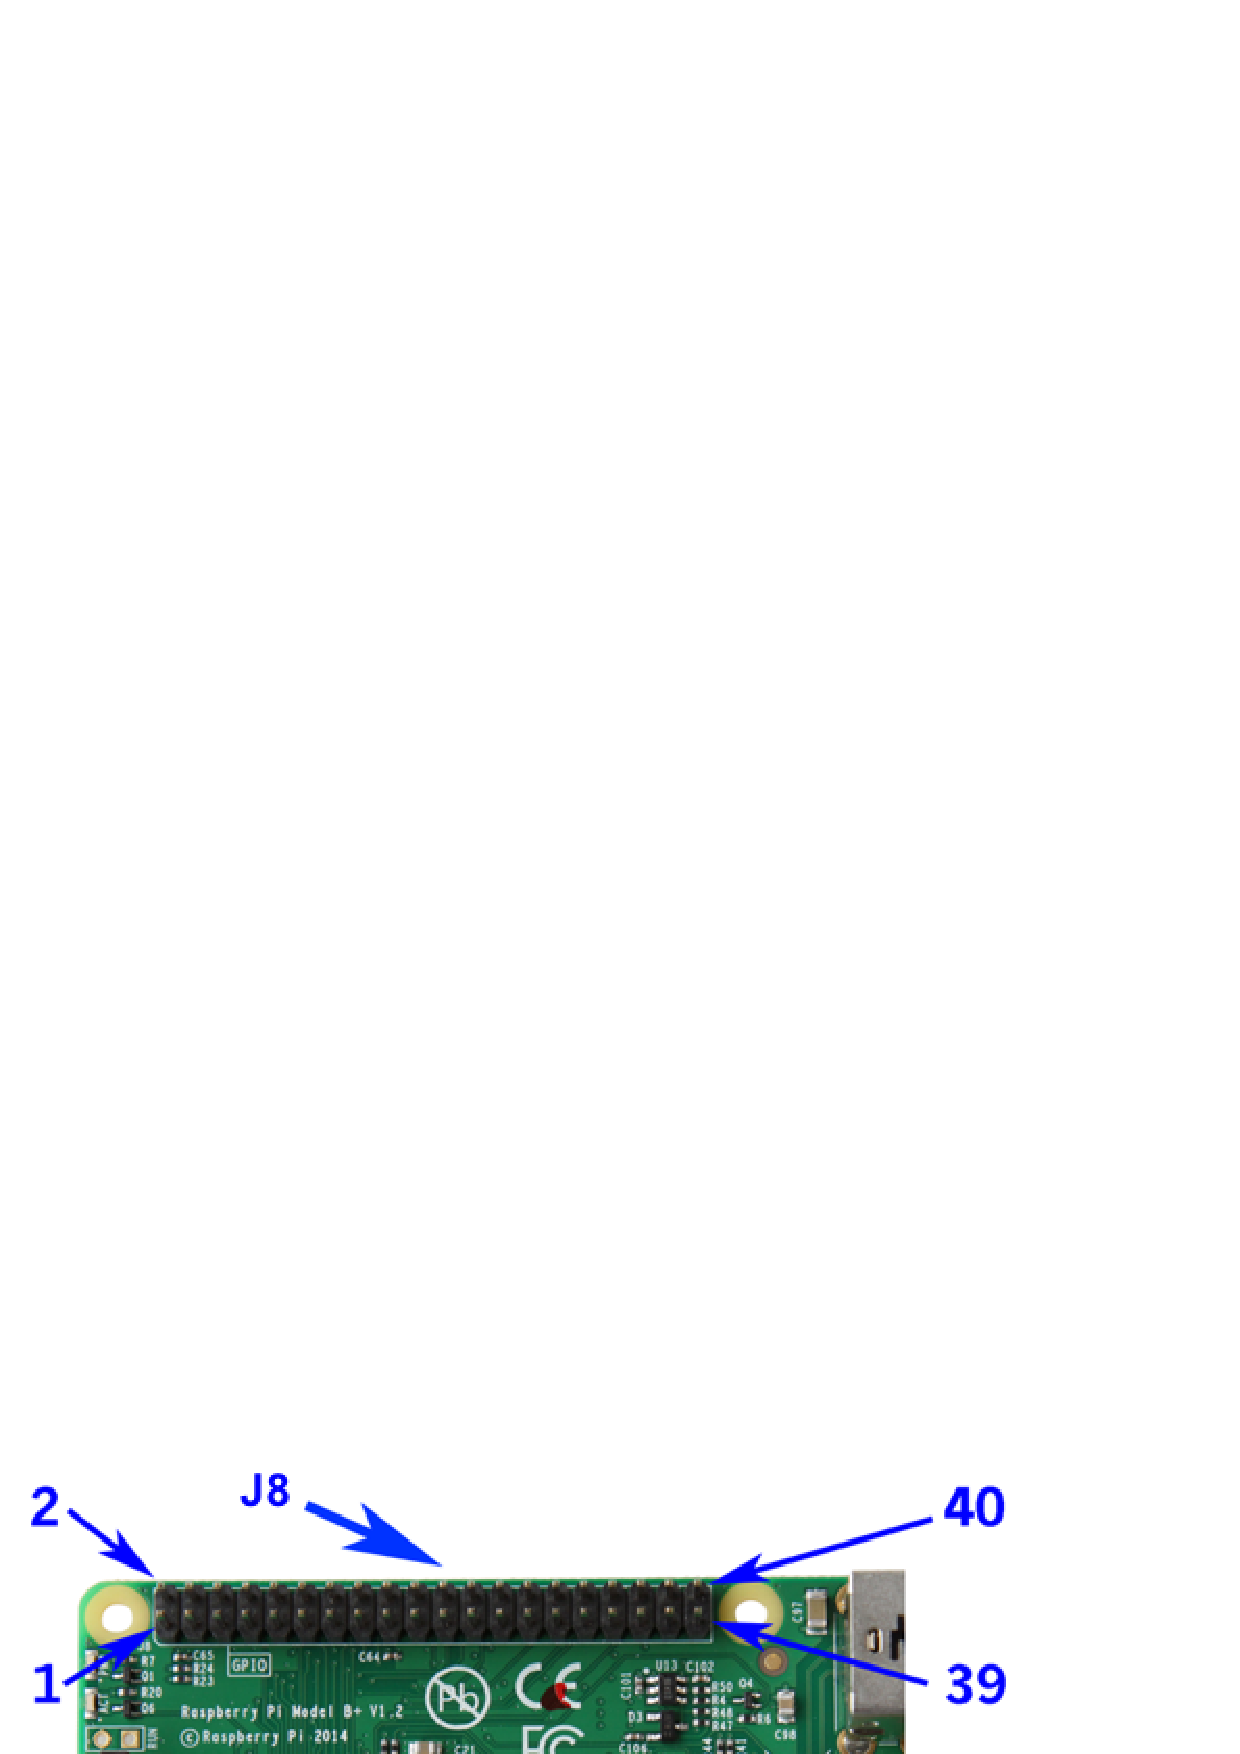
\includegraphics[width=\columnwidth]{./figs/gpio2}
\end{center}
\captionof{figure}{GPIO pin snapshot on Pi.}
\label{fig_1_3a}	
\end{figure}
%
\begin{figure}
\begin{center}
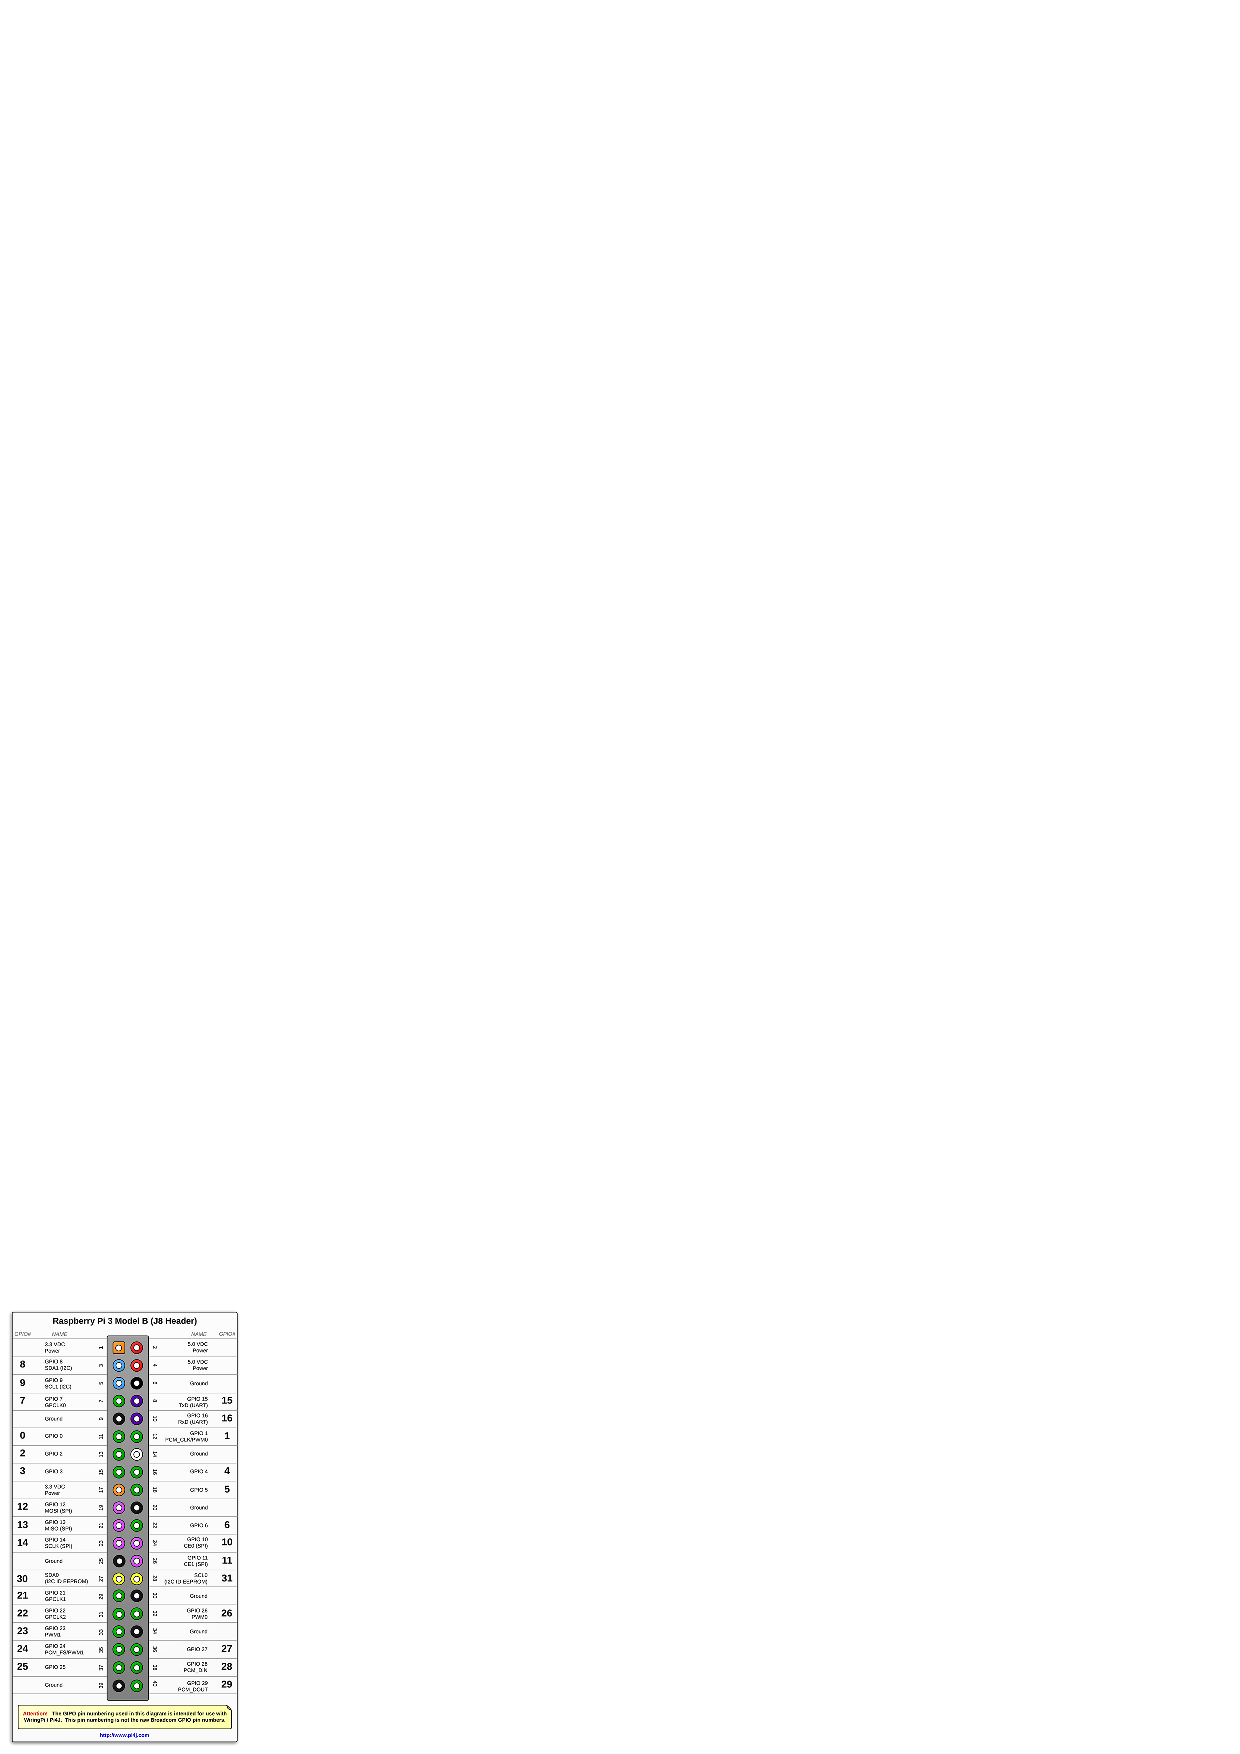
\includegraphics[width=\columnwidth]{./figs/gpio1}
\end{center}
\captionof{figure}{GPIO Wiring Pi pin configuration.}
\label{fig_1_3b}	
\end{figure}
\renewcommand{\thefigure}{\theproblem}
\begin{problem}
Connect the a-g pins of the display to the GPIO pins 0-6 of the Pi shown in \ref{fig_1_3a} and \ref{fig_1_3b}.
\end{problem}
\begin{problem}
Type the following C code and excute. What do you observe?
\end{problem}
\solution
\lstinputlisting[language=C]{./code/seven_seg_disp.c}
\begin{problem}
Now generate the numbers 0-9 by modifying the above program.
\end{problem}
\begin{problem}
Suitably modify the above program to obtain a decade counter.
\end{problem}


%\begin{problem}
%\label{prob:first_code}
%%Type the following code and execute. What do you observe?
%%\lstinputlisting[language=C]{./codes/bcd_seven.c}
%%// the setup function runs once when you press reset or power the board
int a=1,b=0,c=0,d=1,e=1,f=1,g=1;
void setup() {
    pinMode(2, OUTPUT);  
    pinMode(3, OUTPUT);
    pinMode(4, OUTPUT);
    pinMode(5, OUTPUT);
    pinMode(6, OUTPUT);
    pinMode(7, OUTPUT);
    pinMode(8, OUTPUT);            
}

// the loop function runs over and over again forever
void loop() {
  
  digitalWrite(2, a); 
  digitalWrite(3, b); 
  digitalWrite(4, c); 
  digitalWrite(5, d); 
  digitalWrite(6, e); 
  digitalWrite(7, f);     
  digitalWrite(8, g); 
}


%\end{problem}
%\begin{problem}
%Now generate the numbers 0-9 by modifying the above program.
%\end{problem}
%%
%%\newpage

%%\section{Combinational Logic}
%%
%\subsection{Counting Decoder}
	%In the  truth table in Table \ref{table:counter_decoder},  $W,X,Y,Z$ are the inputs
%and $A,B,C,D$ are the outputs. This table represents the system that increments the numbers 0-8 by 1 and resets the number 9 to 0
%%
%Note that  $D = 1$ for the inputs $0111$ and $1000$.  Using {\em boolean} logic,
%%
%\begin{equation}
%\label{bool_logic}
%D = WXYZ^{'} + W^{'}X^{'}Y^{'}Z
%\end{equation}
%%
%Note that $0111$ results in the expression $WXYZ^{'}$ and $1000$ yields $W^{'}X^{'}Y^{'}Z$. 
%%The $\&\&$ operand is used for the boolean AND (multiplication) operation, the $||$ operand is used for the OR (addition) operation and the ! operand is used for the NOT ($^{'}$) operation in Arduino code.  For example, the expression for \eqref{bool_logic} in Arudino is
%%\begin{verbatim}
%%D = (W&&X&&Y&&!Z)||(!W&&!X&&!Y&&Z);
%%\end{verbatim}

%\begin{problem}
	%\label{counter_dec}

%Write the boolean logic functions for $A,B,C$ in terms of $W,X,Y,Z$.
%\end{problem}
%%
%\input{./figs/counter_decoder}
%%
%%
%\begin{problem}
%%	\label{D_code}
%Write a program for implementing Table \ref{counter_dec}.
%%\eqref{bool_logic} in Arduino.
%\end{problem}
%%
%\solution
%%\lstinputlisting[language=C]{./codes/count_decoder.c}
%%
%%\begin{problem}
%%Modify the above program by keeping W=0,X=0,Y=0,Z=1 and A=1 and execute.  Verify that your results are consistent with Table \ref{counter_dec}.
%%\end{problem}

%\begin{problem}
%Verify if your logic is correct by observing the output on the seven segment display for different inputs.
%\end{problem}
%%
%\begin{problem}
%Connect GPIO pin 10 to the dot pin of the display and execute the following code.
%\end{problem}
%%\lstinputlisting[language=C]{./codes/blink.c}
%%
%%
%\begin{problem}
%A decade counter counts the numbers from 0-9 and then resets to 0.  Suitable modify the above programs to obtain a decade counter.
%\end{problem}

%\subsection{Display Decoder}
%%
%\begin{problem}
%Now write the truth table for the seven segment display decoder (IC 7447).  The inputs will be $A,B,C,D$ and the outputs will be $a,b,c,d,e,f,g$.
%\end{problem}
%%
%\begin{problem}
%\label{seven_seg_disp_logic}
%Obtain the logic functions for outputs $a,b,c,d,e,f,g$ in terms of the inputs $A,B,C,D$.
%\end{problem}
%\begin{problem}
%Disconnect the Pi from IC 7447 and connect the pins GPIO 0-6 in the Pi directly to the seven segment display.
%\end{problem}
%\begin{problem}
%Write a new program to implement the logic in Problem \ref{seven_seg_disp_logic} and observe the output in the display.  You have designed the logic for IC 7447!
%\end{problem}
%\begin{problem}
%Now include your counting decoder program in the  display decoder program
%and see if the display shows the consecutive number.
%\end{problem}
%A decade counter counts the numbers from 0-9 and then resets to 0.
%\begin{problem}
%Suitably modify the above program to obtain a decade counter.
%\end{problem}




%\begin{problem}
%Generate the boolean functions for the segments $a-f$ using the table in Problem \ref{bcd_ss}.  For example, the function for $a$ is obtained from the table as
%\begin{equation}
%a=\bar{D}\bar{C}\bar{B}A+\bar{D}C\bar{B}\bar{A}
%\label{boolean}
%\end{equation}
%\end{problem}
%%
%\begin{problem}
	%\label{counter_dec}
%Write functions for $A,B,C,D$ in Arduino using the following table and verify using the Arduino driven display.
		%\input{counter_decoder}
%\end{problem}
%\begin{problem}
	%Write a module for decimal to binary conversion
	%according to the example given below
	%\input{conversion}
	%%
	%$N \% 2$ gives the remainder and $N/2$ gives the quotient
%	and use it in the above code so that decimal values are given as input in the program and observed as output in the display. Note that the following code
%	\begin{verbatim}
%	a % b
%	\end{verbatim}
%	can be used to obtain the remainder when a is divided by b and
%	\begin{verbatim}
%	a/b
%	\end{verbatim}
%	gives the quotient.
%\end{problem}
 
%%
%\newpage
%\section{$M$-ary Modulation}
%\subsection{Angle Bisectors}

\begin{figure}[!h]
	\begin{center}
		
		%
\includegraphics[width=\columnwidth]{./figs/ch3_angle_bisector}
		%\vspace*{-10cm}
		\resizebox{\columnwidth}{!}{\begin{tikzpicture}
[scale=2,>=stealth,point/.style={draw,circle,fill = black,inner sep=0.5pt},]

\node (D) at (0, 0)[point,label=below :$D$] {};
\node (A) at (0, 3)[point,label=above :$A$]{};
\node (B) at (-3, 0)[point,label=below left:$B$]{};
\node (C) at (3, 0)[point,label=below right:$C$]{};
\node (O) at (0, 1.3)[point,label=below right:$O$]{};
\node (F) at (-1.1, 1.9)[point,label=above left:$F$]{};
\node (E) at (1.1, 1.9)[point,label=above right:$E$]{};

\draw (D)--(B);
\draw (B)--(A);
\draw (A)--(C);
\draw (C)--(D);
\draw [thick,dashed] (A) -- (D);
\draw [thick,dashed] (O) -- (E);
\draw [thick,dashed] (O) -- (F);
\draw (B)--(O);
\draw (C)--(O);

\tkzMarkRightAngle[size=.2](A,D,C)
\tkzMarkRightAngle[size=.15](B,F,O);
\tkzMarkRightAngle[size=.15](C,E,O);
\tkzMarkAngle[size=.4](D,B,O);
\tkzMarkAngle[size=.35](O,B,F);
\tkzMarkAngle[size=.54](E,C,O);
\tkzMarkAngle[size=.5](E,C,O);
\tkzMarkAngle[size=.6](O,C,D);
\tkzMarkAngle[size=.65](O,C,D);

\end{tikzpicture}}
	\end{center}
	\caption{Angle bisectors meet at a point}
	\label{ch3_angle_bisector}	
\end{figure}

\begin{definition}
	In Fig. \ref{ch3_angle_bisector}, $OB$ divides the  $\angle B$ into half, i.e.\begin{equation}
	\angle OBC = \angle OBA
	\end{equation}
	$OB$ is known as an angle bisector.
\end{definition}
	$OB$ and $OC$ are angle bisectors of angles $B$ and $C$. $OA$ is joined and $OD, OF$ and $OE$ are perpendiculars to sides $a,b$ and $c$.
\begin{problem}
  Show that $OD = OE = OF$.
\end{problem}
\proof In $\Delta$s $ODC$ and $OEC$,
\begin{align}
OD &= OC \sin \frac{C}{2}
\\
OE &= OC \sin \frac{C}{2} 
\\
\Rightarrow OD &=OE.
\end{align}
Similarly,
\begin{equation}
OD = OF.
\end{equation}
%
\begin{problem}
	Show that OA is the angle bisector of $\angle A$
\end{problem}
\proof In $\Delta$s $OFA$ and $OEA$,
\begin{align}
OF &= OE
\\
\Rightarrow OA \sin OAF &= OA \sin OAE \\
\Rightarrow \sin OAF &=  \sin OAE \\
\Rightarrow \angle OAF &= \angle OAE
\end{align}
which proves that $OA$ bisects $\angle A$.
{\em Conclusion:} The angle bisectors of a triangle meet at a point.


\subsection{Congruent Triangles}
%
\begin{problem}
	Show that in $\Delta$s $ODC$ and $OEC$, corresponding sides and angles are equal.
\end{problem}
\begin{definition}
	Note that    $\Delta$s $ODC$ and $OEC$ are known as congruent triangles.  To show that two triangles are congruent, it is sufficient to show that some angles and sides are equal.
\end{definition}
\begin{problem}
SSS:	Show that if the corresponding sides of three triangles are equal, the triangles are congruent.
\end{problem}
\begin{problem}
ASA:	Show that if two angles and any one side  are equal in corresponding triangles, the triangles are congruent.
\end{problem}
\begin{problem}
SAS:	Show that if two sides and the angle between them are equal in corresponding triangles, the triangles are congruent.
\end{problem}
\begin{problem}
RHS:	For two right angled triangles, if the hypotenuse and one of the sides are equal, show that the triangles are congruent.
\end{problem}
	%
%%
\subsection{Perpendicular Bisectors}
\begin{definition}
	In Fig. \ref{ch3_perp_bisector}, OD $\perp BC$ and $BD=DC$. $OD$ is defined as the perpendicular bisector of $BC$.
\end{definition}

\begin{problem}
	In Fig. \ref{ch3_perp_bisector}, show that $OA=OB=OC$.
\end{problem}
%%
%%
\begin{figure}[!h]
	\begin{center}
		
		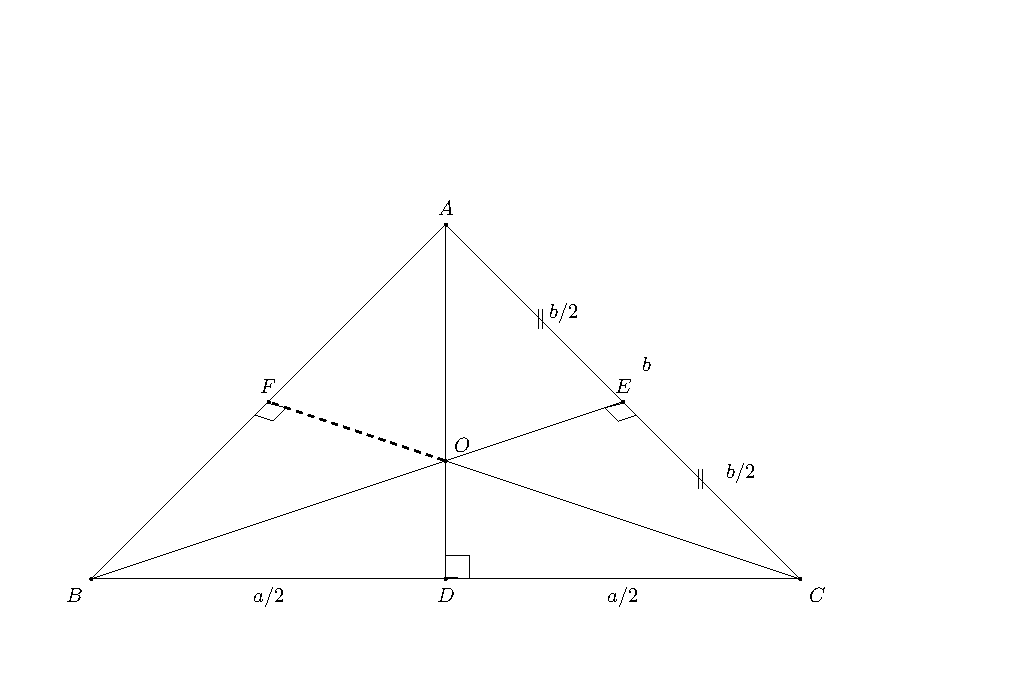
\includegraphics[width=\columnwidth]{./figs/fig_3.8.eps}
%		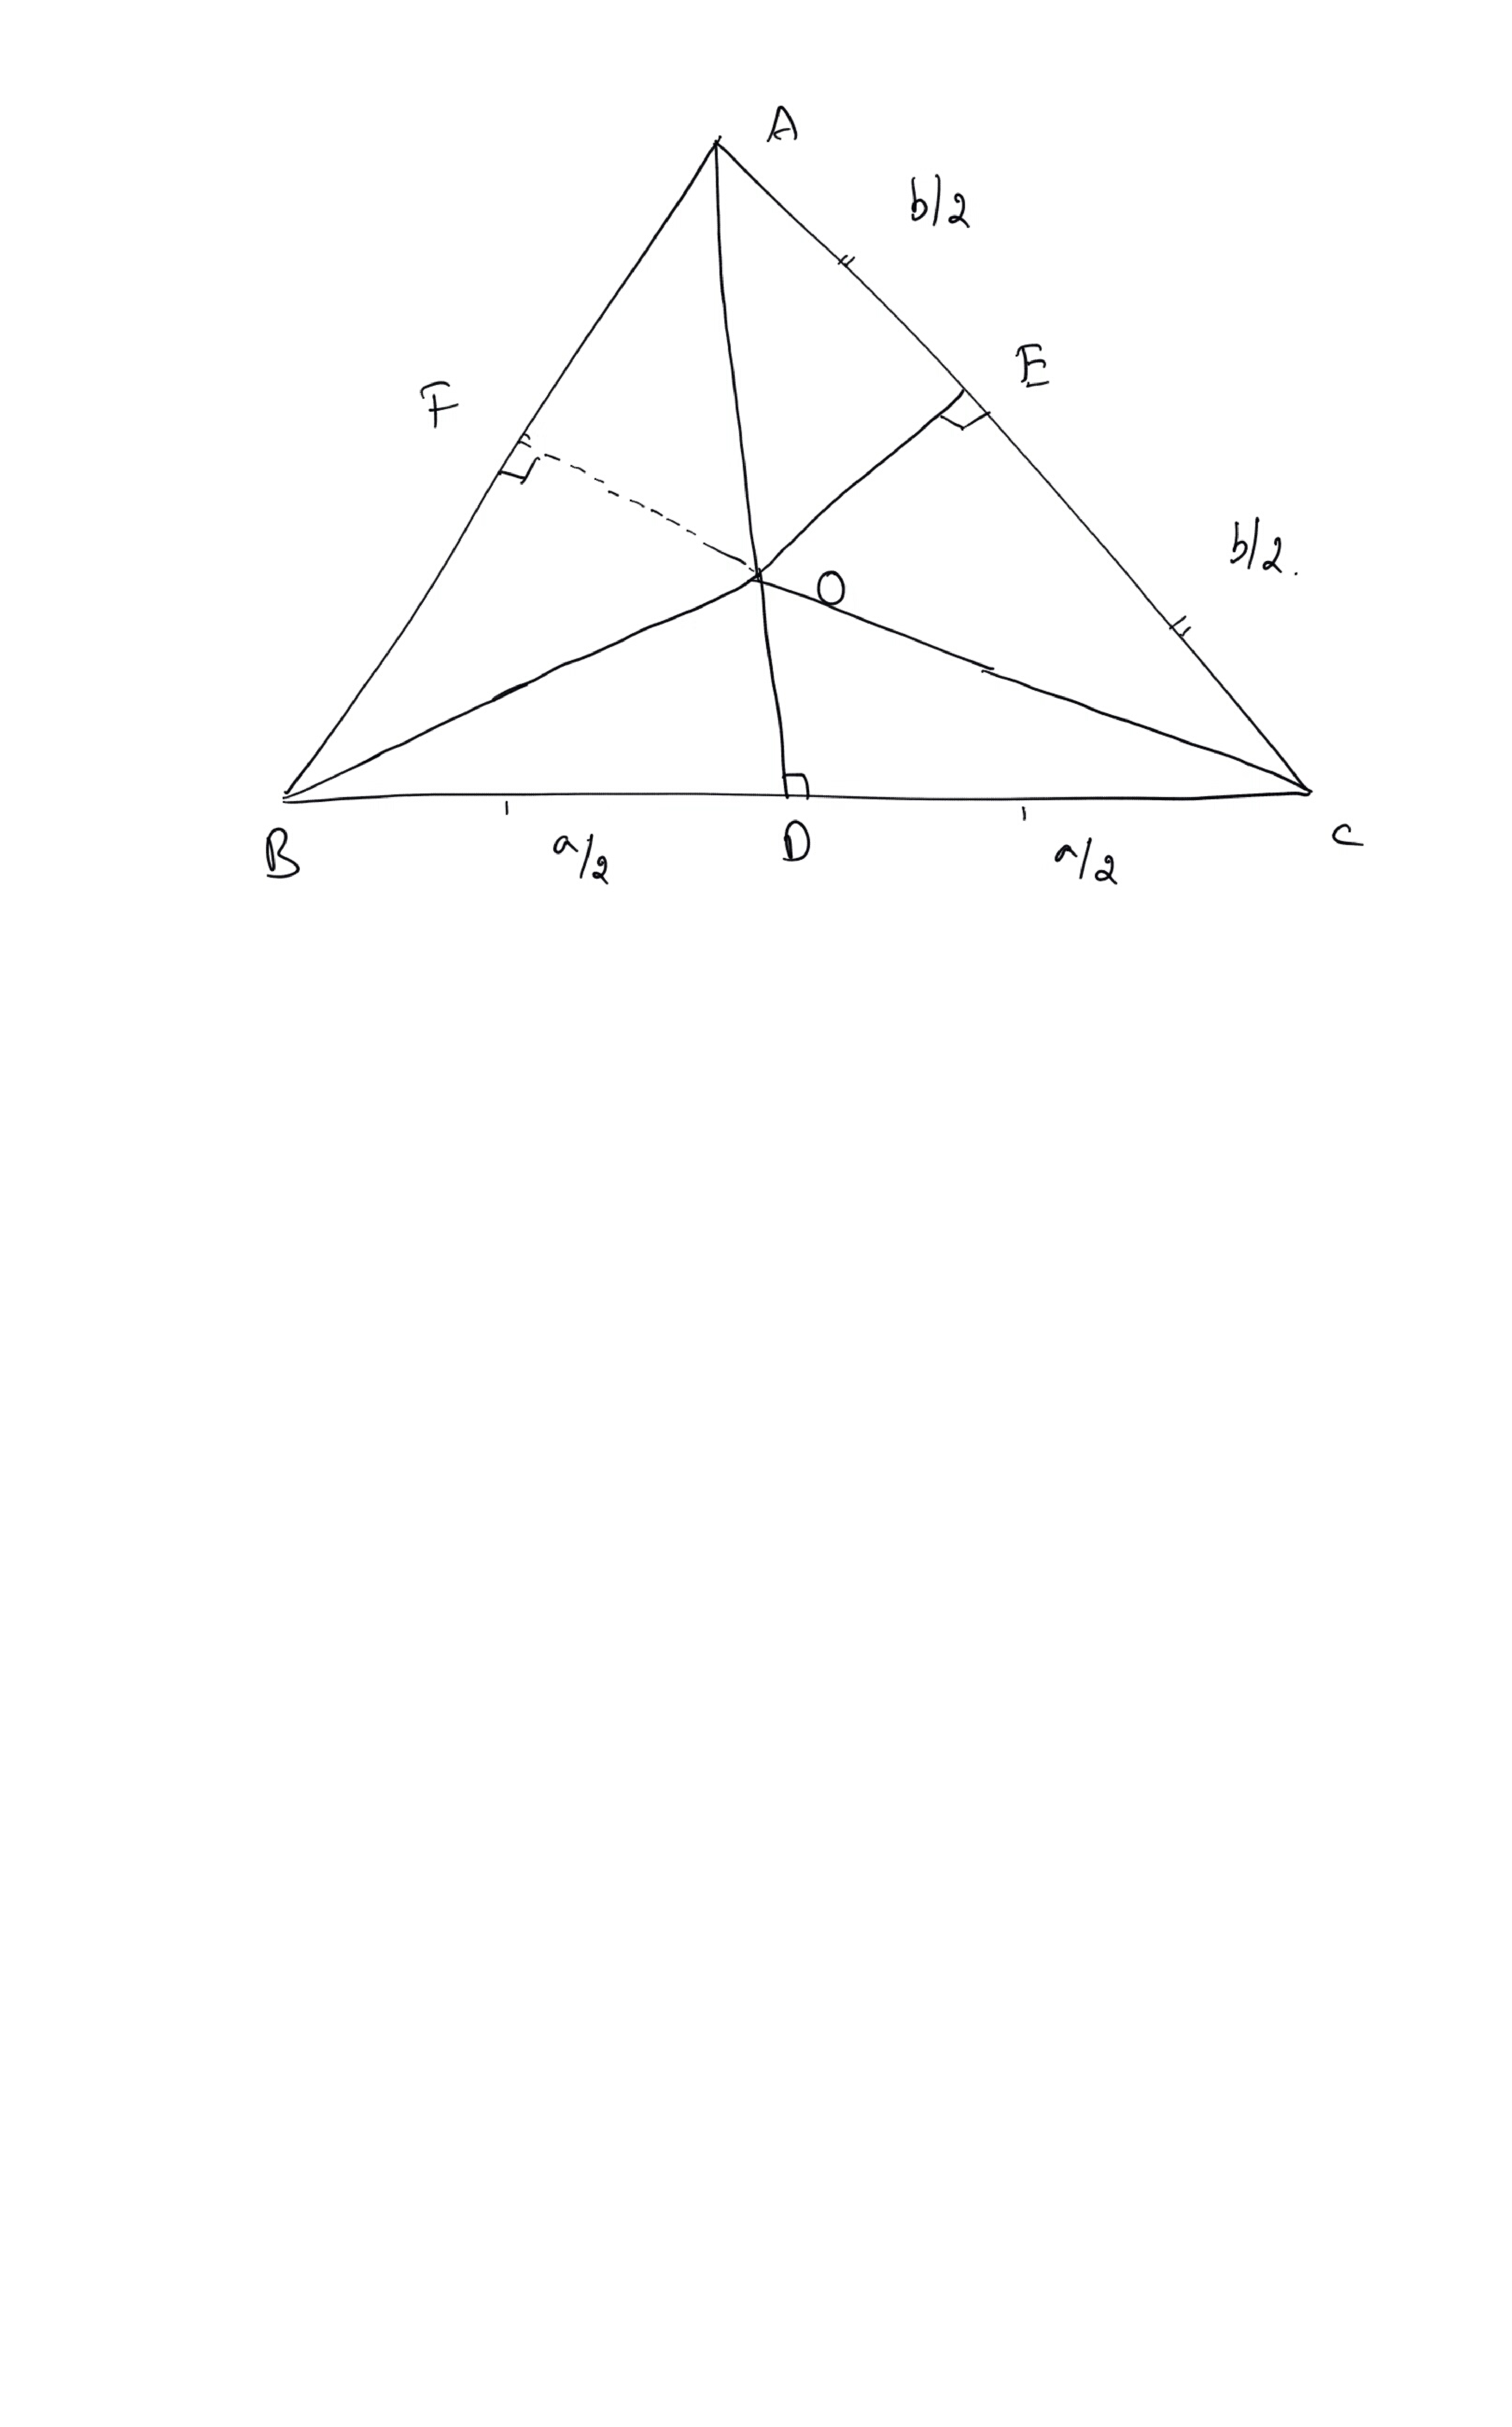
\includegraphics[width=\columnwidth]{./figs/ch3_perp_bisector}
		%\vspace*{-10cm}
%		\resizebox{\columnwidth}{!}{\documentclass{standalone}
\usepackage{tikz}
\usepackage{tkz-euclide}
\usetkzobj{all}
%\usepackage{amsmath}
\providecommand{\brak}[1]{\ensuremath{\left(#1\right)}}

\begin{document}
\begin{tikzpicture}
[scale=2,>=stealth,point/.style={draw,circle,fill = black,inner sep=0.5pt},]

\node (E) at (1.5, 1.5)[point,label=above :$E$] {};
\node (F) at (-1.5, 1.5)[point,label=above :$F$] {};
\node (A) at (0, 3)[point,label=above :$A$]{};
\node (B) at (-3, 0)[point,label=below left:$B$]{};
\node (C) at (3, 0)[point,label=below right:$C$]{};
\node (D) at (0,0)[point,label=below :$D$] {};
\node (O) at (0,1)[point,label=above right :$O$] {};


\draw (B)--(A);
\draw (A)--(C);
\draw (B)--(C);
\draw (B)--(E);
\draw (C)--(O);
\draw (A)--(D);
\draw [thick,dashed] (O) -- (F);

\node [above] at (1.7,1.7) {$b$};
\node [above] at (2.5,.75) {$b/2$};
\node [above] at (1,2.1) {$b/2$};
\node [above] at (-1.5,-0.3){$a/2$};
\node [above] at (1.5,-0.3){$a/2$};
\tkzMarkRightAngle[size=.16](B,F,O)
\tkzMarkRightAngle[size=.16](C,E,O)
\tkzMarkRightAngle[size=.2](A,D,C)
\draw   -- (4.3,1.7) node[midway] {$\parallel$};
\draw   -- (1.6,4.4) node[midway] {$\parallel$};

\end{tikzpicture}
\end{document}}
	\end{center}
	\caption{Perpendicular bisectors meet at a point}
	\label{ch3_perp_bisector}	
\end{figure}
%
\proof In $\Delta$s $ODB$ and $ODC$, using Budhayana's theorem,
%
\begin{equation}
\begin{split}
OB^2 &= OD^2 + BD^2 \\
OC^2 &= OD^2 + DC^2 
\end{split}
\end{equation}
%
Since $BD = DC = \frac{a}{2}$, $OB = OC$.  Similarly, it can be shown that $OA = OC$.  Thus, $OA=OB=OC$.
%
\begin{definition}
	In $\Delta AOB$, $OA = OB$.  Such a triangle is known as an isoceles triangle.
\end{definition}
%
\begin{problem}
	Show that $AF = BF$.
\end{problem}
\proof Trivial using Budhayana's theorem.  This shows that $OF$ is a perpendicular bisector of $AB$. 
{\em Conclusion:}  The perpendicular bisectors of a triangle meet at a point.
%
\subsection{Perpendiculars from Vertex to Opposite Side}
	%
	%
	In Fig. \ref{ch3_perp_triang}, $AD \perp BC$ and $BE \perp AC$. $CF$ passes through $O$ and meets
	$AB$ at $F$.  	
\begin{problem}
	Show that 
	\begin{align}
	OE = c \cos A \cot C
	\end{align}
\end{problem}
	\begin{figure}[!h]
		\begin{center}
			
			%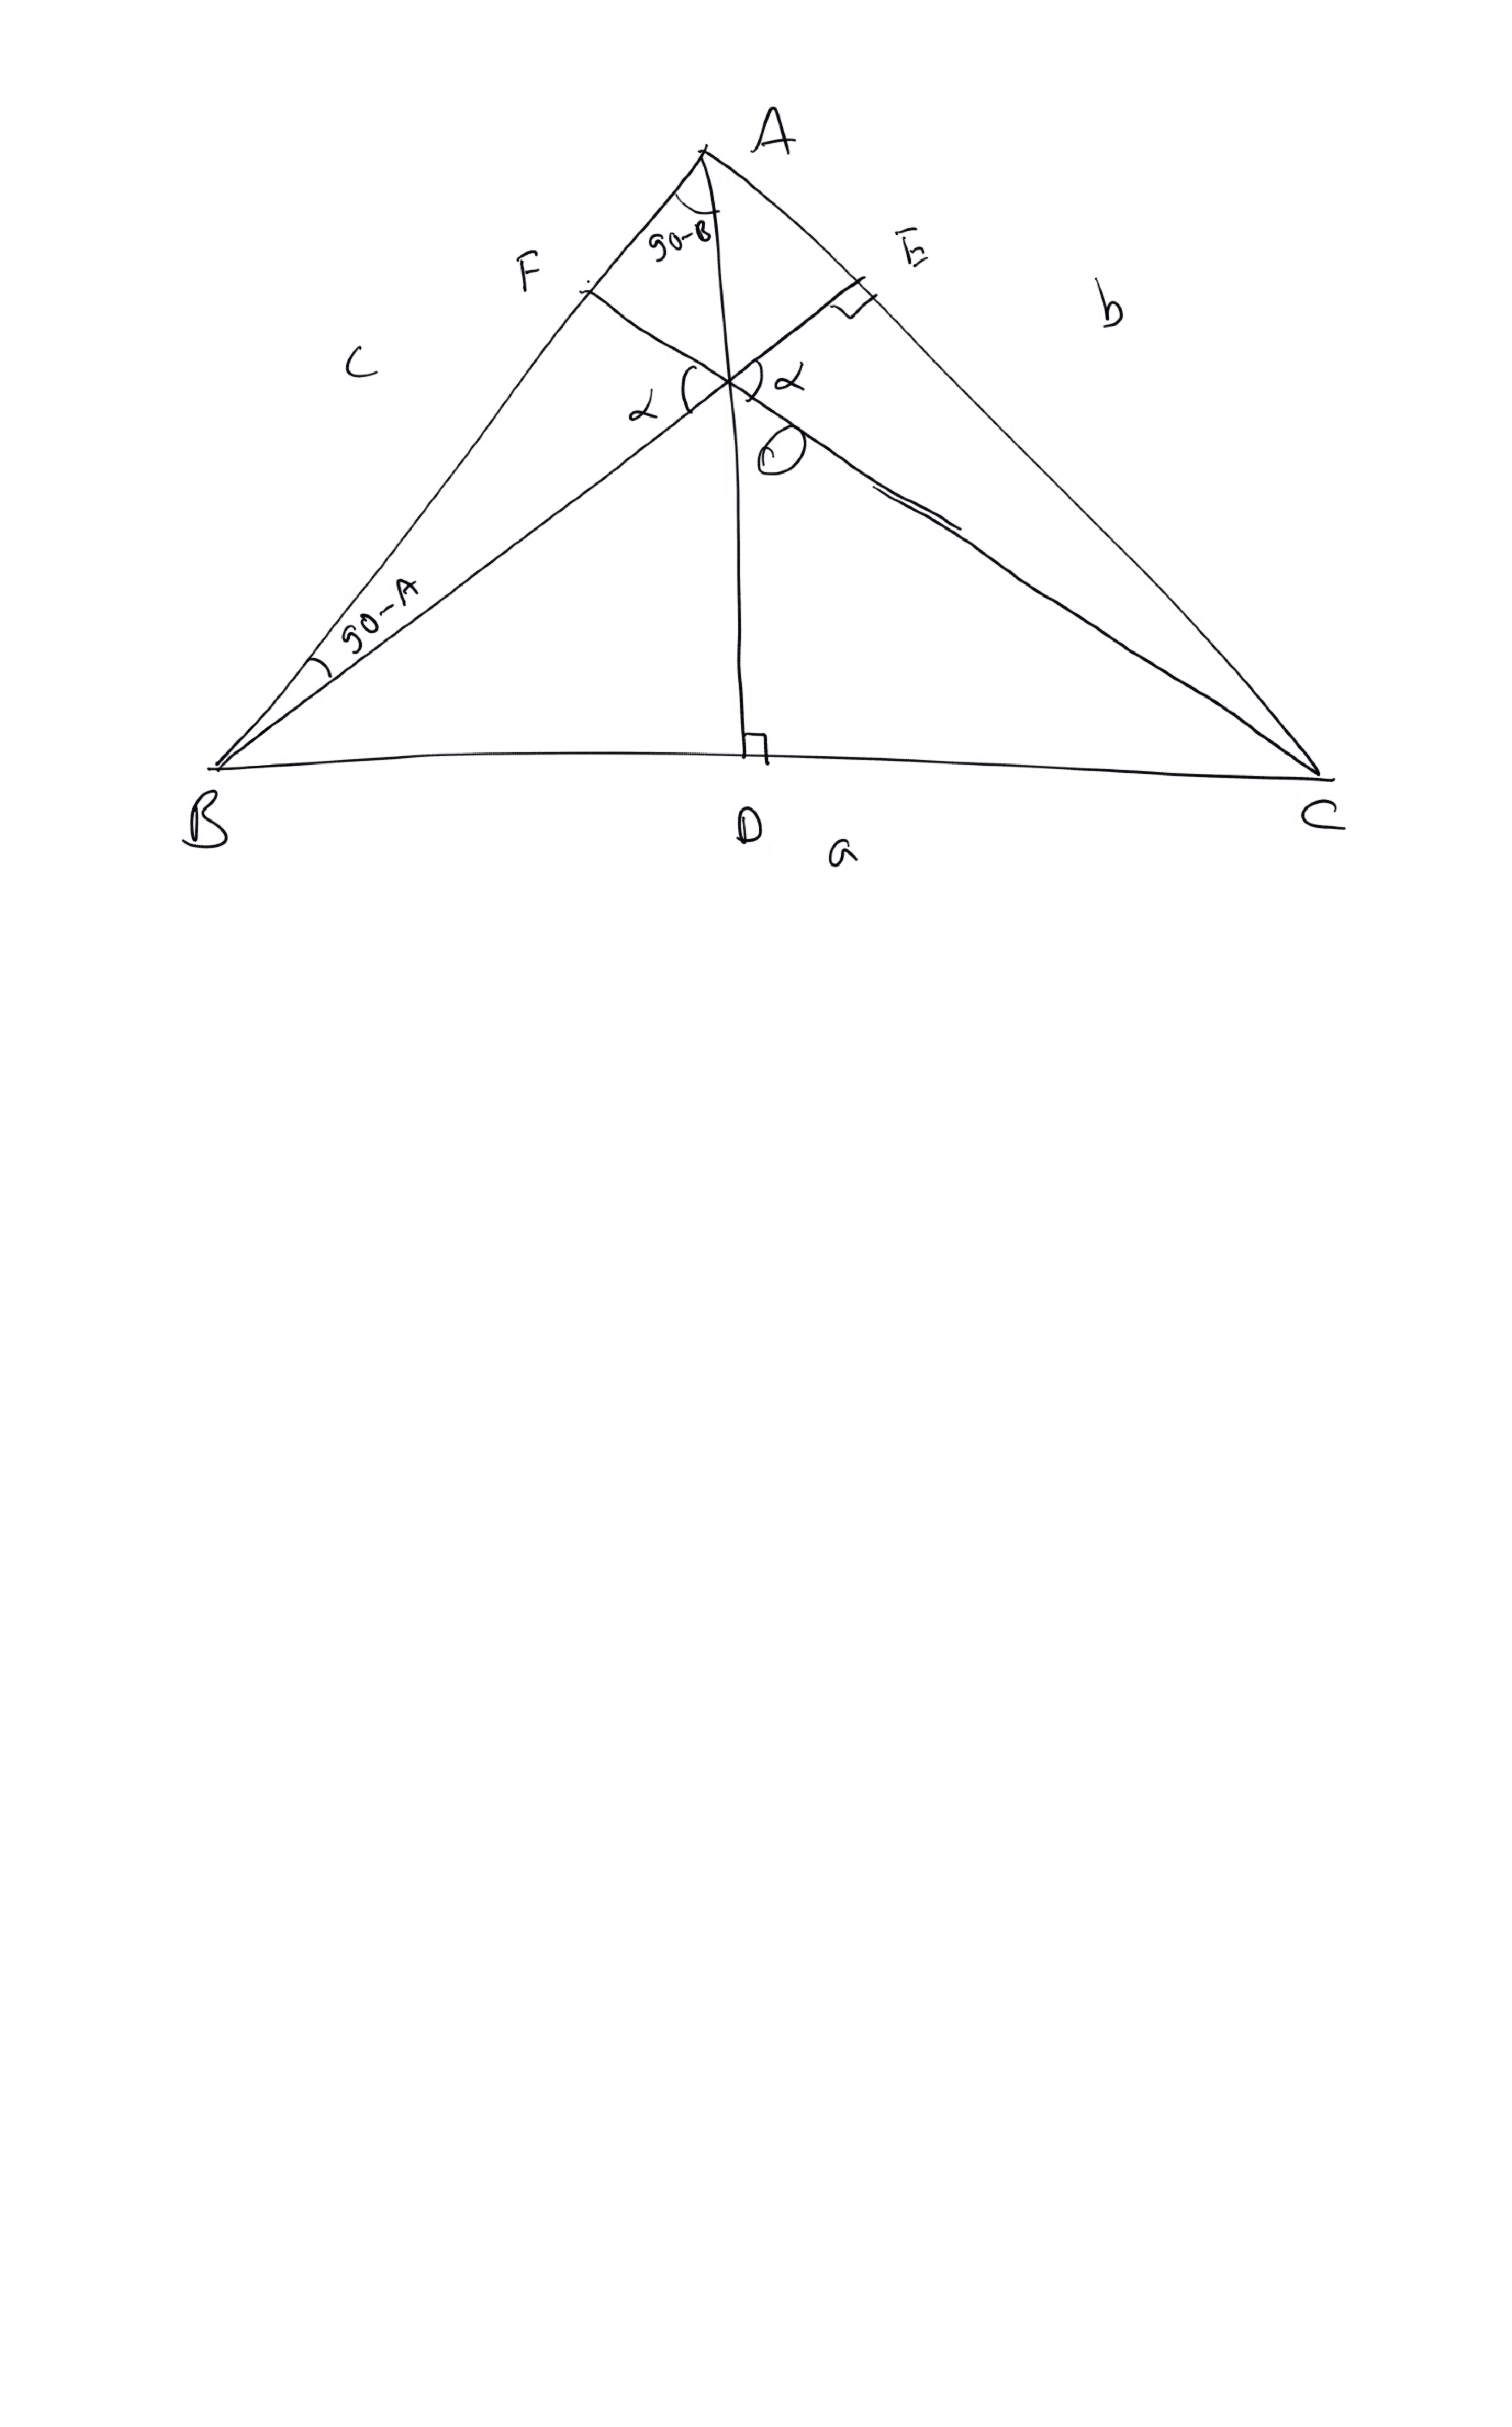
\includegraphics[width=\columnwidth]{./figs/ch3_perp_triang}
			%\vspace*{-10cm}
			\resizebox{\columnwidth}{!}{\begin{tikzpicture}
[scale=2,>=stealth,point/.style={draw,circle,fill = black,inner sep=0.5pt},]

\node (E) at (1.5, 1.5)[point,label=above :$E$] {};
\node (F) at (-1.5, 1.5)[point,label=above :$F$] {};
\node (A) at (0, 3)[point,label=above :$A$]{};
\node (B) at (-3, 0)[point,label=below left:$B$]{};
\node (C) at (3, 0)[point,label=below right:$C$]{};
\node (O) at (0,1)[point,label=above right :$O$] {};
\node (D) at (0,0)[point,label=below :$D$] {};


\draw (B)--(A);
\draw (A)--(C);
\draw (B)--(E);
\draw (C)--(F);
\draw (B)--(C);
\draw (A)--(D);

\node [below] at (0,-0.3) {$a$};
\node [above] at (-1.7,1.7) {$c$};
\node [above] at (1.7,1.7) {$b$};
\node [above] at (1,1.3) {$p$};
\node [above] at (-1,1.3) {$q$};
\node [above] at (-2.3,0.24){\rotatebox{45}{$90-A$}};
\node [above] at (-0.4,2.1) {\rotatebox{45}{$90-B$}};
\node [above] at (0.4,2.1) {\rotatebox{-45}{$90-C$}};

\tkzMarkAngle[size=.3](F,O,B);
\tkzMarkAngle[size=.3](C,O,E);
\tkzMarkAngle[size=.4](O,B,F);
\tkzMarkAngle[size=.2](F,A,O);
\tkzMarkAngle[size=.3](O,A,E);
\draw (-0.5,1) node{$\alpha$};
\draw (0.5,1) node{$\alpha$};

\end{tikzpicture}
}
		\end{center}
		\caption{Perpendiculars from vertex to opposite side meet at a point}
		\label{ch3_perp_triang}	
	\end{figure}
%
\proof In $\Delta$ s $AEB$ and $AEO$,
%
\begin{align}
AE &= c \cos A \\
OE &= AE \tan \brak{90^{\degree} - C} \brak{\because ADC \text{ is right angled}} \\
&= AE \cot C
\end{align}
%
From both the above, we get the desired result.
%
\begin{problem}
	Show that $\alpha = A$.
\end{problem}
\proof In $\Delta OEC$,
%
\begin{equation}
CE = a \cos C \brak{\because BEC \text{ is right angled}}
\end{equation}
%
Hence,
%
\begin{equation}
\begin{split}
\tan \alpha &= \frac{CE}{OE} \\
&=  \frac{a \cos C}{c \cos A \cot C} \\
&=  \frac{a \cos C \sin C}{c \cos A \cos C} \\
&= \frac{a \sin C}{c \cos A } \\
&= \frac{c \sin A}{c \cos A } \brak{\because \frac{a}{\sin A} = \frac{c}{\sin C}}\\
&= \tan A\\
\Rightarrow \alpha = A
\end{split}
\end{equation}
%
\begin{problem}
	Show that $CF \perp AB$
\end{problem}
\proof Consider triangle OFB and the result of the previous problem.  $\because$ the sum of the angles of a triangle is $180^{\degree}$, $\angle CFB = 90^{\degree}$.
{\em Conclusion: The perperdiculars from the vertex of a triangle to the opposite side meet at a point.} 
%
%\newpage
%\section{BER in Rayleigh Flat Slowly Fading Channels}
	%\subsection{Chord of a Circle}

\begin{figure}[!h]
	\begin{center}
		
		
\includegraphics[width=\columnwidth]{./figs/ch4_circle_def}
		\vspace*{-10cm}
	\end{center}
	\caption{Circle Definitions}
	\label{ch4_circle_def}	
\end{figure}
\begin{definition}
	Fig. \ref{ch4_circle_def} represents a circle.  The points in the circle are at a distance $r$ from the centre $O$.  $r$ is known as the radius.
\end{definition}

\subsection{Chords of a circle}
\begin{definition}
	In Fig. \ref{ch4_circle_def}, $A$ and $B$ are points on the circle.  The line $AB$ is known as a chord of the circle.
\end{definition}
%
%
\begin{problem}
	\label{ch4_prob_circle_subtend}
	In Fig. \ref{ch4_circle_subtend}  Show that $\angle OAB = 2\angle APB $.
\end{problem}
\begin{figure}[!h]
	\begin{center}
		
		
\includegraphics[width=\columnwidth]{./figs/ch4_circle_subtend}
		\vspace*{-10cm}
	\end{center}
	\caption{Angle subtended by chord $AB$ at the centre $O$ is twice the angle subtended at $P$. }
	\label{ch4_circle_subtend}	
\end{figure}

\proof In Fig. \ref{ch4_circle_subtend}, the triangeles $OPA$ and $OPB$ are isosceles. Hence,
%
\begin{align}
\angle OPB = \angle OBP &= \theta_1 \\
\angle OPA = \angle OAP &= \theta_2
\end{align}
%
Also, $\alpha$ and $\beta$ are exterior angles corresponding to the triangle $OPB$ and $OPA$ respectively. Hence
%
\begin{align}
\alpha &= 2\theta_1 \\
\beta &= 2\theta_2
\end{align}
%
Thus,
%
\begin{align}
\angle AOB &= \alpha + \beta \\
&= \theta_1 + \theta_2 \\
&= \angle APB
\end{align}
%
\begin{definition}
	The diameter of a circle is the chord that divides the circle into two equal parts. In Fig. \ref{ch4_circle_dia}, $AB$ is the diameter and passes through the centre $O$
\end{definition}
%
\begin{problem}
In Fig. \ref{ch4_circle_dia}, show that $\angle APB = 90^{\degree}$ .
\end{problem}
%
\begin{figure}[!h]
	\begin{center}
		
		
\includegraphics[width=\columnwidth]{./figs/ch4_circle_dia}
		\vspace*{-10cm}
	\end{center}
	\caption{Diameter of a circle.}
	\label{ch4_circle_dia}	
\end{figure}

\begin{problem}
	In Fig. \ref{ch4_chord_product}, show that 
	\begin{equation}
	\begin{split}
\angle ABD &= \angle ACD \\
\angle CAB &= \angle CDB	
	\end{split}
	\end{equation}
\end{problem}
\begin{figure}[!h]
	\begin{center}
		
		
\includegraphics[width=\columnwidth]{./figs/ch4_chord_product}
		\vspace*{-10cm}
	\end{center}
	\caption{$PA.PB = PC.PD$}
	\label{ch4_chord_product}	
\end{figure}
%
%
\proof Use Problem \ref{ch4_prob_circle_subtend}.
%
\begin{problem}
	In Fig. \ref{ch4_chord_product}, show that the triangles $PAB$ and $PBD$ are similar
\end{problem}
\proof Trivial using previous problem
\begin{problem}
	In Fig. \ref{ch4_chord_product}, show that 
	\begin{equation}
	PA.PB = PC.PD
	\end{equation}
\end{problem}
%
\proof Since triangles $PAC$ and $PBD$ are similar, 
%
\begin{align}
\frac{PA}{PD} &= \frac{PC}{PB} \\
\Rightarrow PA.PB &= PC.PD
\end{align}
%
%
\begin{definition}
	The line $PX$ in Fig. \ref{ch4_tangent_def} touches the circle at exactly one  point $P$. It is known as the tangent to the circle.
\end{definition}
%
%
\begin{problem}
	$OP$ is the perpendicular to the line $PX$ as shown in the Fig. \ref{ch4_short_dist}. Show that $OP$ is the shortest distance between the point $O$ and the line $PX$. 
\end{problem}
\proof Let $P_1$ be a point on the line $PX$. Then $OPP_1$ is a right angled triangle.  Using Budhayana's theorem,
%
\begin{figure}[!h]
	\begin{center}
		
		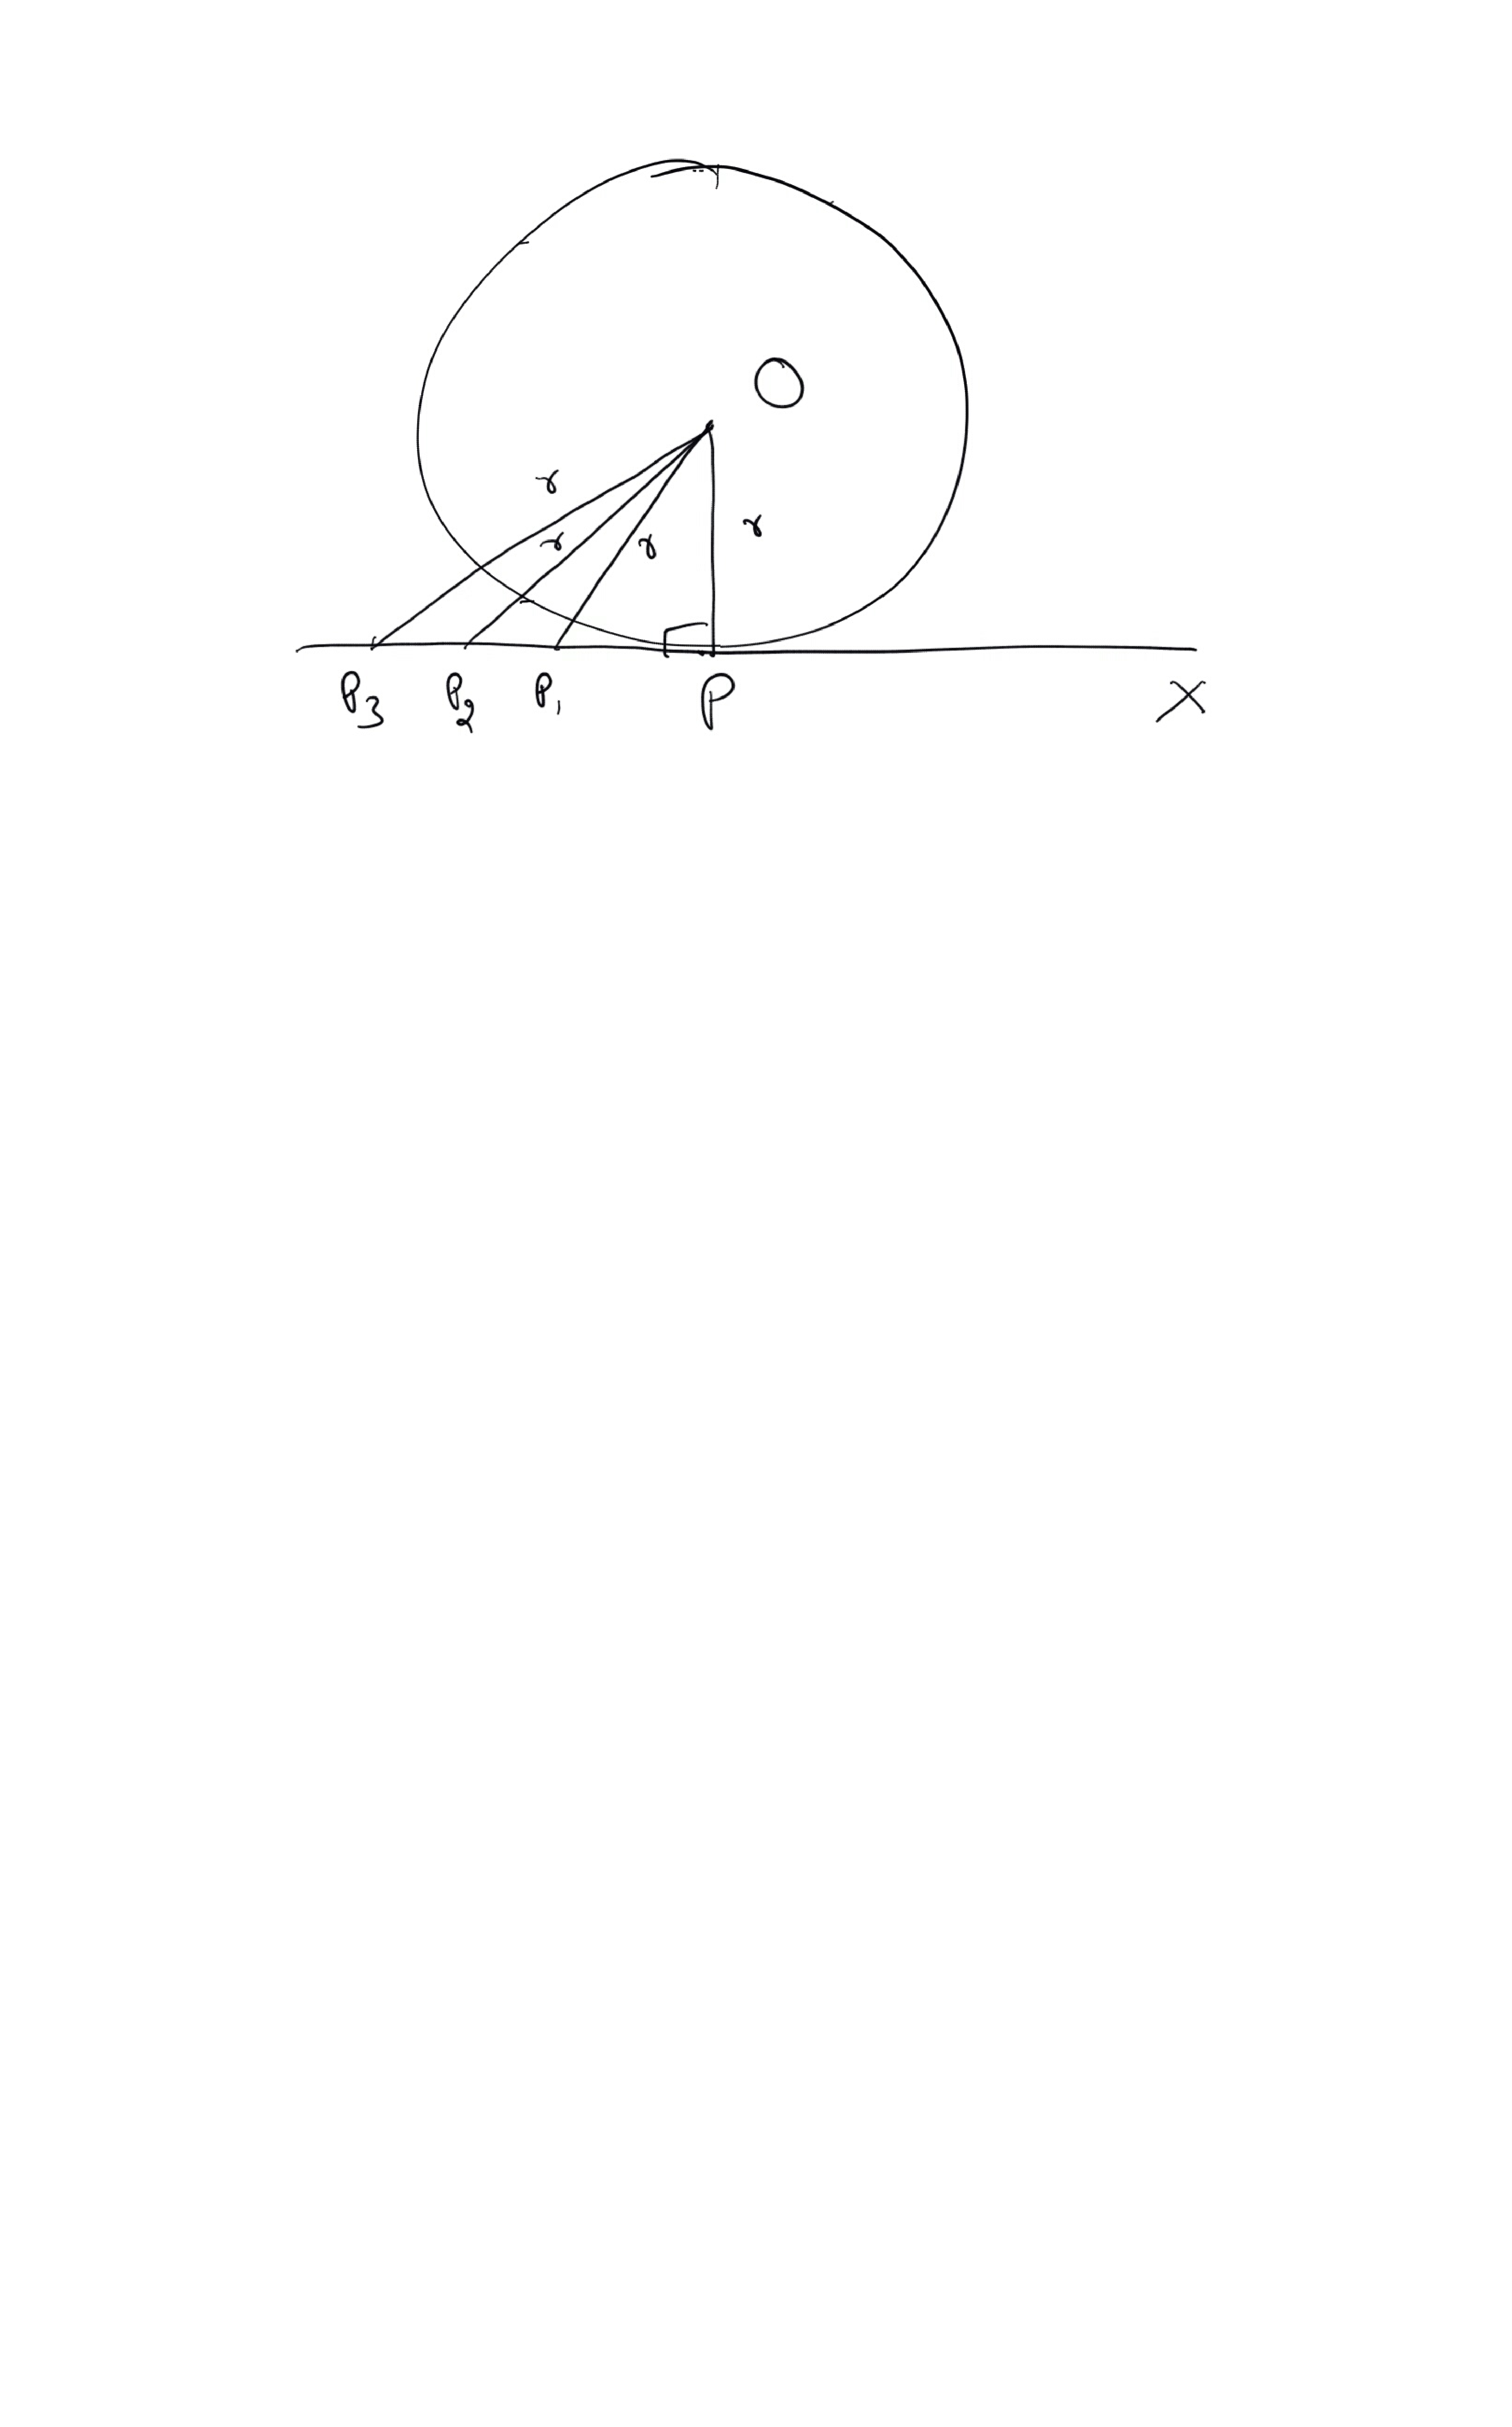
\includegraphics[width=\columnwidth]{./figs/ch4_tangent_def}
		\vspace*{-10cm}
	\end{center}
	\caption{Tangent to a Circle.}
	\label{ch4_tangent_def}	
\end{figure}
%
\begin{figure}[!h]
	\begin{center}
		
		
\includegraphics[width=\columnwidth]{./figs/ch4_short_dist}
		\vspace*{-10cm}
	\end{center}
	\caption{Shortest distance from $O$ to line $PX$}
	\label{ch4_short_dist}	
\end{figure}

%
\begin{equation}
\begin{split}
OP_1^2 &= OP^2 + PP_1^2 \\
\Rightarrow OP_1 > OP
\end{split}
\end{equation}
%
Thus, $OP$ is the shortest distance between $O$ and line $PX$.
%
\begin{problem}
Show that $\angle OPX = 90 ^{\degree}$
\end{problem}
\proof In Fig. \ref{ch4_tangent_def}, we can see that $OP$ is is the radius of the circle and the length of all line segments from $O$ to the line $PX > r$.  Using the result of the previous 
problem, it is obvious that $OP \perp PX$. 
%
	%
\begin{problem}
In Fig. \ref{ch4_tangent_prod} show that 
%
\begin{equation}
\angle PCA = \angle PBC
\end{equation}
%
$O$ is the centre of the circle and $PC$ is the tangent.
\end{problem}
	\begin{figure}[!h]
		\begin{center}
			
			
\includegraphics[width=\columnwidth]{./figs/ch4_tangent_prod}
			\vspace*{-10cm}
		\end{center}
		\caption{$PA.PB = PC^2$.}
		\label{ch4_tangent_prod}	
	\end{figure}
	%

%
\proof For convenience, greek letters are used for representing certain angles. Since $\Delta OAC$ is isosceles,
%
\begin{align}
2 \alpha + 2 \brak{\beta - \phi} &= 180^{\degree} \\
\Rightarrow  \alpha +  \brak{\beta - \phi} &= 90^{\degree} \\
\Rightarrow  \alpha +  \beta  &= 90^{\degree} + \phi
\end{align}
%
Since $theta$ is an exterior angle for the $\Delta ABC
$,
%
\begin{equation}
\theta = \alpha + \beta
\end{equation}
%
From both the above equations
%
\begin{equation}
\theta = 90^{\degree} + \phi
\end{equation}
%
Since PC is the tangent, 
%
\begin{equation}
\angle PCB = 90^{\degree} + \phi = \theta
\end{equation}
%
Considering the sum of angles in $\Delta PAC$ $\Delta PBC$,
%
\begin{align}
\angle P + \theta + \angle PCA &= 180^{\degree} \\
\angle P + \theta + \alpha &= 180^{\degree}
\end{align}
Hence,
%
\begin{equation}
\angle PCA = \alpha
\end{equation}
%
\begin{problem}
	In Fig. \ref{ch4_tangent_prod}, show that the triangles $PAC$ and $PBC$ are similar.
\end{problem}
\proof From the previous problem, it is obvious that corresponding angles of both triangles are equal.  Hence they are similar.
%
\begin{problem}
	Show that $PA.PB = PC^2$
\end{problem}
\proof Since $\Delta PAC \sim \Delta PBC$, their sides are in the same ratio.  Hence,
%
\begin{align}
\frac{PA}{PC} &= \frac{PC}{PB} \\
\Rightarrow PA.PB &=PC^2
\end{align}
%
%
\begin{problem}
	In Fig. \ref{ch4_chord_tangent_prod}, show that\begin{equation}
	PA.PB = PC.PD
	\end{equation}
\end{problem}
%
\begin{figure}[!h]
	\begin{center}
		
		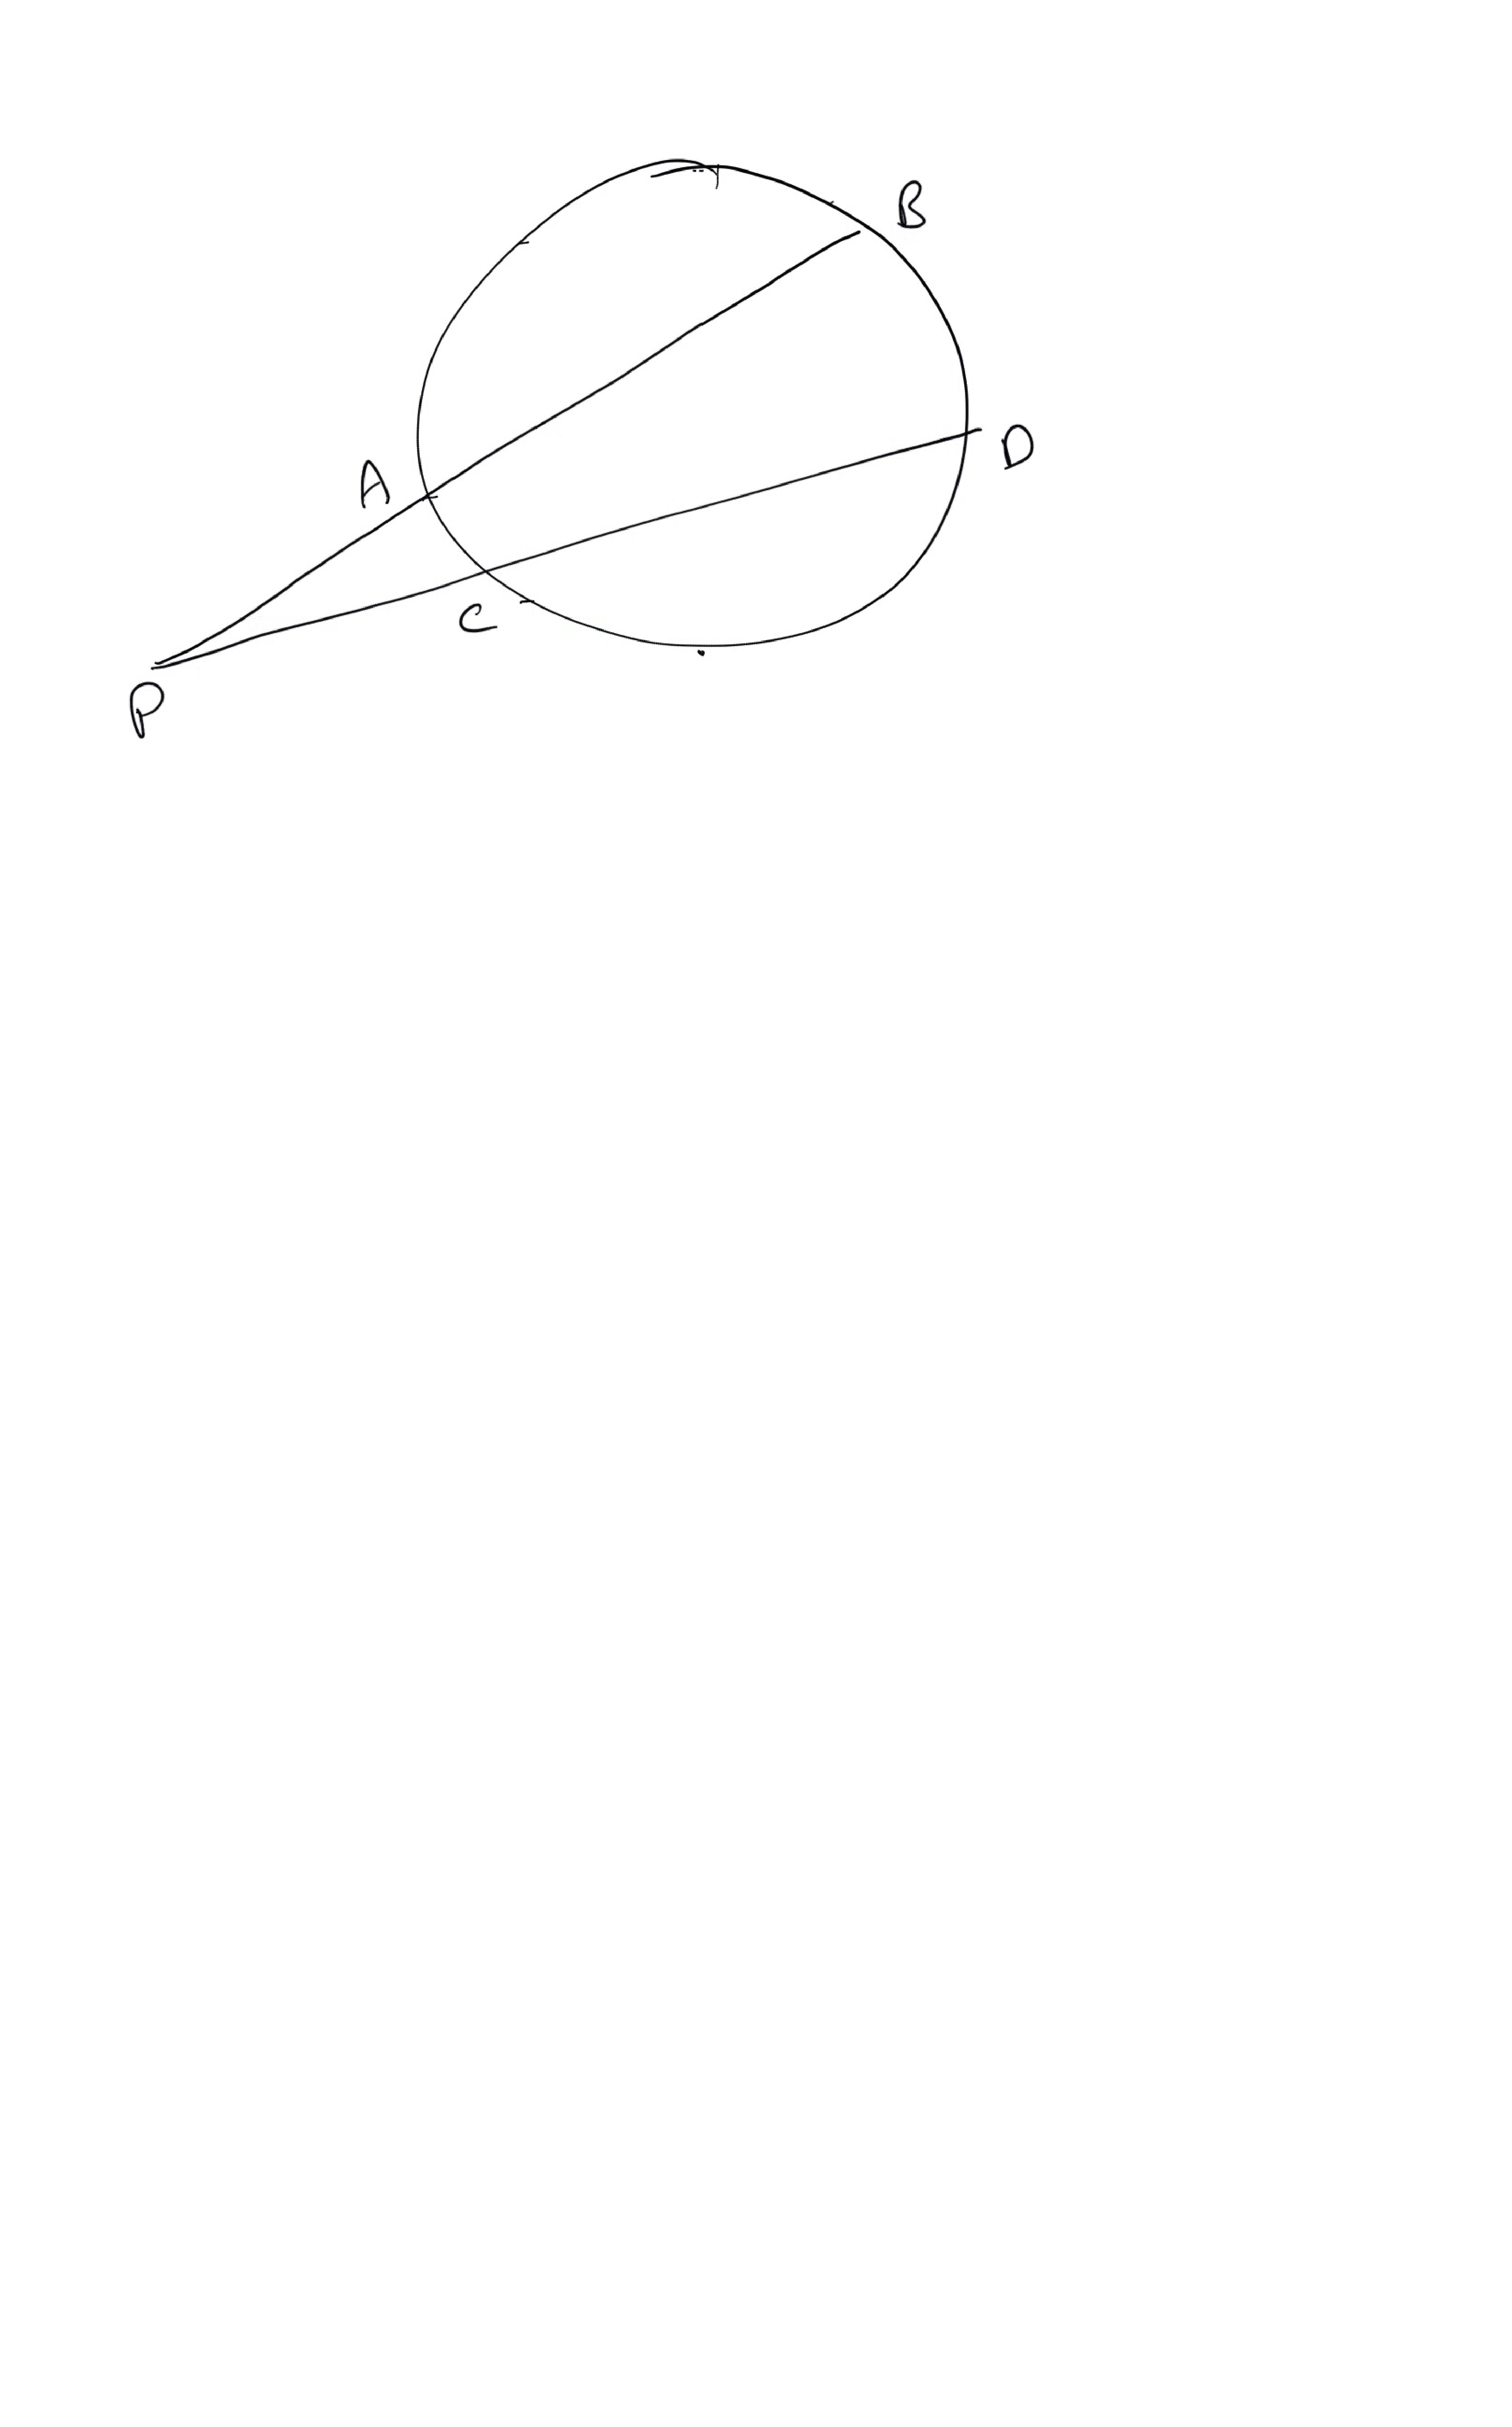
\includegraphics[width=\columnwidth]{./figs/ch4_chord_tangent_prod}
		\vspace*{-10cm}
	\end{center}
	\caption{$PA.PB = PC^2$.}
	\label{ch4_chord_tangent_prod}	
\end{figure}

\proof Draw a tangent and use the previous problem.
 




 
\subsection{Example}
\renewcommand{\theequation}{\theenumi}

\begin{enumerate}[label=\arabic*.,ref=\thesubsection.\theenumi]
\item In $\triangle ABC$,
\begin{equation}
\label{eq:linea}
\vec{A}=\myvec{1\\2}
\end{equation}
%
and the equations of the medians through $\vec{B}$ and $\vec{C}$
are respectively
\begin{align}
\label{eq:line_medb}
\myvec{1 & 1}\vec{x}&=5
\\
\myvec{1 & 0}\vec{x}&=4
\label{eq:line_medc}
\end{align}
%
Find the area of $\triangle ABC$.
\\
\solution The centroid $\vec{O}$ is the solution of \eqref{eq:line_medb},\eqref{eq:line_medc} and is obtained 
as the solution
of the matrix equation
\begin{align}
\myvec{1 & 1 \\1 & 0}\vec{x}&=\myvec{5 \\ 4}
\label{eq:line_matrix}
\end{align}
%
which can be solved using the augmented matrix as follows.
\begin{align}
\myvec{1 & 1 & 5\\1 & 0 & 4} \leftrightarrow \myvec{1 & 1 & 5\\0 & 1 & 1}\leftrightarrow  \myvec{1 & 0 & 4\\0 & 
1 & 1}
\end{align}
Thus,
\begin{equation}
\label{eq:lineo}
\vec{O}=\myvec{4\\1}
\end{equation}
% 
Let  $AD$ be the median through $\vec{A}$. Then,
\begin{align}
\frac{\vec{A}+\vec{B}+\vec{C}}{3}&= \vec{O}
\\
\implies \vec{B}+\vec{C}= 3\vec{O}-\vec{A} &= \myvec{11 \\ 1}
\label{eq:line_b+c}
\\
\implies \myvec{1 & 1}\vec{B}+\myvec{1 & 1}\vec{C}&=  \myvec{1 & 1}\myvec{11 \\ 1}
\label{eq:line_ctemp}
\end{align}
%
From \eqref{eq:line_medc} and \eqref{eq:line_ctemp},
\begin{align}
 \myvec{1 & 1}\vec{B} &= 5 
\\
\implies 5+\myvec{1 & 1}\vec{C}&=  12
\\
\implies \myvec{1 & 1}\vec{C}&=  7
\label{eq:line_ctemp2}
\end{align}
From \eqref{eq:line_ctemp2} and \eqref{eq:line_medc}, $\vec{C}$ can be obtained by solving 
\begin{align}
\myvec{1 & 1 \\1 & 0}\vec{C}&=\myvec{7 \\ 4}
\label{eq:line_cmatrix}
\end{align}
using the augmented matrix as
\begin{align}
\myvec{1 & 1 & 7\\1 & 0 & 4} &\leftrightarrow \myvec{1 & 1 & 7\\0 & 1 & 3}\leftrightarrow \myvec{1 & 0 & 4\\0 & 
1 & 3}
\\
\implies \vec{C}&=\myvec{4\\3}
\end{align}
%
From \eqref{eq:line_b+c},
\begin{align}
\vec{B}&=\myvec{11\\1}-\myvec{4\\3}
=\myvec{7\\-2}
\end{align}
%
Thus,
\begin{align}
\frac{1}{2}
\begin{vmatrix}
\vec{A} & \vec{B} &\vec{C}
\\
1 & 1 & 1
\end{vmatrix}
=
\frac{1}{2}
\begin{vmatrix}
1 & 7 & 4\\2 & -2 & 3 \\ 1 & 1 & 1
\end{vmatrix} = 9
\end{align}
\item Summarize all the above computations through a Python script and plot $\triangle ABC$.
\\
\solution
\begin{lstlisting}
https://github.com/gadepall/school/raw/master/linalg/2D/manual/codes/triang.py
\end{lstlisting}
\begin{figure}
\centering
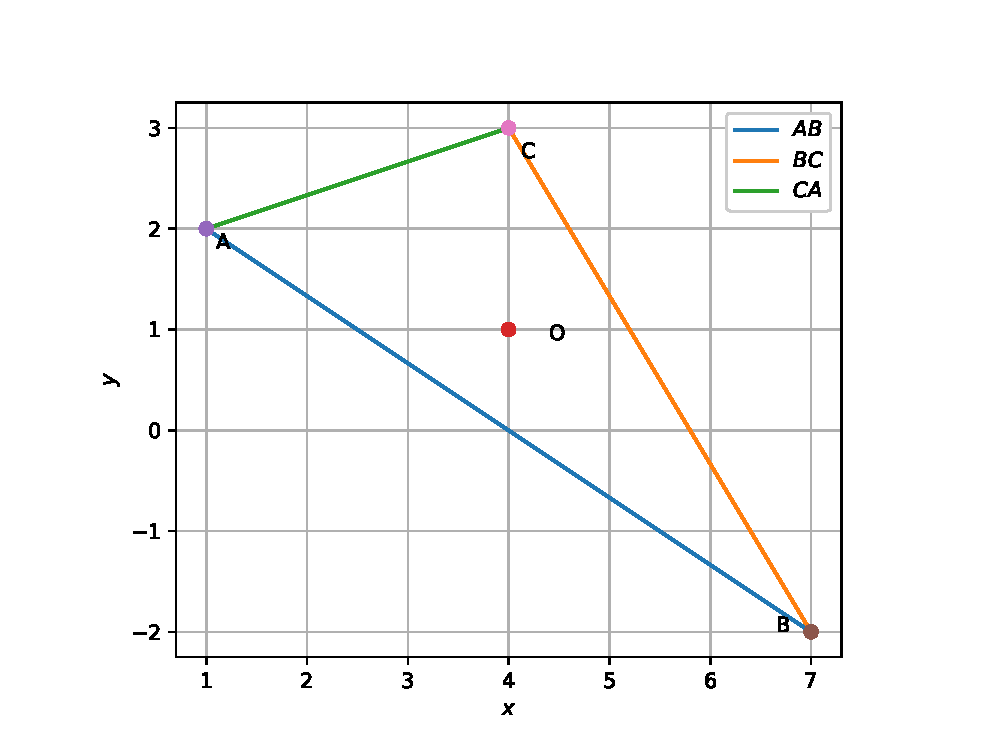
\includegraphics[width=\columnwidth]{./line/figs/triangle.eps}
\caption{}
\label{fig:triangle}
\end{figure}


%\numberwithin{equation}{enumi}

%\renewcommand{\theequation}{\theenumi}
\end{enumerate}
.
 
\subsection{Programming}
\renewcommand{\theequation}{\theenumi}

\begin{enumerate}[label=\arabic*.,ref=\thesubsection.\theenumi]
\numberwithin{equation}{enumi}
\item
Find the {\em orthocentre} of  $\triangle ABC$.
\\
\solution The following code finds the required point using \eqref{eq:alt_ap} and \eqref{eq:alt_bq}
.
\begin{lstlisting}
codes/2d/orthocentre.py
\end{lstlisting}

\item Find $\vec{P}$, the foot of the altitude from $\vec{A}$ upon BC.
%
\\
\solution 
\begin{lstlisting}
codes/2d/alt_foot.py
\end{lstlisting}
\item Find $\vec{Q}$ and $\vec{R}$.
\item Draw $AP, BQ$ and $CR$ and verify that they meet at a point 
$\vec{H}$.  
\\
\solution The following code plots the altitudes in Fig. \ref{fig:alt_triangle}
\begin{lstlisting}
codes/2d/alt_draw.py
\end{lstlisting}
\begin{figure}
\centering
\includegraphics[width=\columnwidth]{./line/figs/alt_triangle.eps}
\caption{}
\label{fig:alt_triangle}
\end{figure}
\item
Find the coordinates of $\vec{D}, \vec{E}$ and $\vec{F}$ of the mid points of $AB, BC$ and $CA$ respectively 
for  $\Delta ABC$. 
\item
Find the equations of $AD,BE$ and $CF$. 
%
\item
\label{prob:median}
Find the point of intersection of $AD$ and $CF$.
\item
Verify that $\vec{O}$ is the point of intersection of $BE,CF$ as 
well.
%as
\item
Graphically show that the medians of $\Delta ABC$ meet at the centroid.
\end{enumerate}

 
\subsection{Exercises}
%\documentclass[journal,12pt,twocolumn]{IEEEtran}
%\usepackage{setspace}
%\usepackage{gensymb}
%\usepackage{caption}
%%\usepackage{multirow}
%%\usepackage{multicolumn}
%%\usepackage{subcaption}
%%\doublespacing
%\singlespacing
%\usepackage{csvsimple}
%\usepackage{amsmath}
%\usepackage{multicol}
%%\usepackage{enumerate}
%\usepackage{amssymb}
%%\usepackage{graphicx}
%\usepackage{newfloat}
%%\usepackage{syntax}
%\usepackage{listings}
%\usepackage{iithtlc}
%\usepackage{color}
%\usepackage{tikz}
%\usetikzlibrary{shapes,arrows}
%
%
%
%%\usepackage{graphicx}
%%\usepackage{amssymb}
%%\usepackage{relsize}
%%\usepackage[cmex10]{amsmath}
%%\usepackage{mathtools}
%%\usepackage{amsthm}
%%\interdisplaylinepenalty=2500
%%\savesymbol{iint}
%%\usepackage{txfonts}
%%\restoresymbol{TXF}{iint}
%%\usepackage{wasysym}
%\usepackage{amsthm}
%\usepackage{mathrsfs}
%\usepackage{txfonts}
%\usepackage{stfloats}
%\usepackage{cite}
%\usepackage{cases}
%\usepackage{mathtools}
%\usepackage{caption}
%\usepackage{enumerate}	
%\usepackage{enumitem}
%\usepackage{amsmath}
%%\usepackage{xtab}
%\usepackage{longtable}
%\usepackage{multirow}
%%\usepackage{algorithm}
%%\usepackage{algpseudocode}
%\usepackage{enumitem}
%\usepackage{mathtools}
%\usepackage{hyperref}
%%\usepackage[framemethod=tikz]{mdframed}
%\usepackage{listings}
%    %\usepackage[latin1]{inputenc}                                 %%
%    \usepackage{color}                                            %%
%    \usepackage{array}                                            %%
%    \usepackage{longtable}                                        %%
%    \usepackage{calc}                                             %%
%    \usepackage{multirow}                                         %%
%    \usepackage{hhline}                                           %%
%    \usepackage{ifthen}                                           %%
%  %optionally (for landscape tables embedded in another document): %%
%    \usepackage{lscape}     
%
%
%\usepackage{url}
%\def\UrlBreaks{\do\/\do-}
%
%
%%\usepackage{stmaryrd}
%
%
%%\usepackage{wasysym}
%%\newcounter{MYtempeqncnt}
%\DeclareMathOperator*{\Res}{Res}
%%\renewcommand{\baselinestretch}{2}
%\renewcommand\thesection{\arabic{section}}
%\renewcommand\thesubsection{\thesection.\arabic{subsection}}
%\renewcommand\thesubsubsection{\thesubsection.\arabic{subsubsection}}
%
%\renewcommand\thesectiondis{\arabic{section}}
%\renewcommand\thesubsectiondis{\thesectiondis.\arabic{subsection}}
%\renewcommand\thesubsubsectiondis{\thesubsectiondis.\arabic{subsubsection}}
%
%% correct bad hyphenation here
%\hyphenation{op-tical net-works semi-conduc-tor}
%
%%\lstset{
%%language=C,
%%frame=single, 
%%breaklines=true
%%}
%
%%\lstset{
%	%%basicstyle=\small\ttfamily\bfseries,
%	%%numberstyle=\small\ttfamily,
%	%language=Octave,
%	%backgroundcolor=\color{white},
%	%%frame=single,
%	%%keywordstyle=\bfseries,
%	%%breaklines=true,
%	%%showstringspaces=false,
%	%%xleftmargin=-10mm,
%	%%aboveskip=-1mm,
%	%%belowskip=0mm
%%}
%
%%\surroundwithmdframed[width=\columnwidth]{lstlisting}
%\def\inputGnumericTable{}                                 %%
%\lstset{
%%language=C,
%frame=single, 
%breaklines=true,
%columns=fullflexible
%}
% 
%
%\begin{document}
%%
%\tikzstyle{block} = [rectangle, draw,
%    text width=3em, text centered, minimum height=3em]
%\tikzstyle{sum} = [draw, circle, node distance=3cm]
%\tikzstyle{input} = [coordinate]
%\tikzstyle{output} = [coordinate]
%\tikzstyle{pinstyle} = [pin edge={to-,thin,black}]
%
%\theoremstyle{definition}
%\newtheorem{theorem}{Theorem}[section]
%\newtheorem{problem}{Problem}
%\newtheorem{proposition}{Proposition}[section]
%\newtheorem{lemma}{Lemma}[section]
%\newtheorem{corollary}[theorem]{Corollary}
%\newtheorem{example}{Example}[section]
%\newtheorem{definition}{Definition}[section]
%%\newtheorem{algorithm}{Algorithm}[section]
%%\newtheorem{cor}{Corollary}
%\newcommand{\BEQA}{\begin{eqnarray}}
%\newcommand{\EEQA}{\end{eqnarray}}
%\newcommand{\define}{\stackrel{\triangle}{=}}
%
%\bibliographystyle{IEEEtran}
%%\bibliographystyle{ieeetr}
%
%\providecommand{\nCr}[2]{\,^{#1}C_{#2}} % nCr
%\providecommand{\nPr}[2]{\,^{#1}P_{#2}} % nPr
%\providecommand{\mbf}{\mathbf}
%\providecommand{\pr}[1]{\ensuremath{\Pr\left(#1\right)}}
%\providecommand{\qfunc}[1]{\ensuremath{Q\left(#1\right)}}
%\providecommand{\sbrak}[1]{\ensuremath{{}\left[#1\right]}}
%\providecommand{\lsbrak}[1]{\ensuremath{{}\left[#1\right.}}
%\providecommand{\rsbrak}[1]{\ensuremath{{}\left.#1\right]}}
%\providecommand{\brak}[1]{\ensuremath{\left(#1\right)}}
%\providecommand{\lbrak}[1]{\ensuremath{\left(#1\right.}}
%\providecommand{\rbrak}[1]{\ensuremath{\left.#1\right)}}
%\providecommand{\cbrak}[1]{\ensuremath{\left\{#1\right\}}}
%\providecommand{\lcbrak}[1]{\ensuremath{\left\{#1\right.}}
%\providecommand{\rcbrak}[1]{\ensuremath{\left.#1\right\}}}
%\theoremstyle{remark}
%\newtheorem{rem}{Remark}
%\newcommand{\sgn}{\mathop{\mathrm{sgn}}}
%\providecommand{\abs}[1]{\left\vert#1\right\vert}
%\providecommand{\res}[1]{\Res\displaylimits_{#1}} 
%\providecommand{\norm}[1]{\lVert#1\rVert}
%\providecommand{\mtx}[1]{\mathbf{#1}}
%\providecommand{\mean}[1]{E\left[ #1 \right]}
%\providecommand{\fourier}{\overset{\mathcal{F}}{ \rightleftharpoons}}
%%\providecommand{\hilbert}{\overset{\mathcal{H}}{ \rightleftharpoons}}
%\providecommand{\system}{\overset{\mathcal{H}}{ \longleftrightarrow}}
%	%\newcommand{\solution}[2]{\textbf{Solution:}{#1}}
%\newcommand{\solution}{\noindent \textbf{Solution: }}
%\newcommand{\myvec}[1]{\ensuremath{\begin{pmatrix}#1\end{pmatrix}}}
%\providecommand{\dec}[2]{\ensuremath{\overset{#1}{\underset{#2}{\gtrless}}}}
%\DeclarePairedDelimiter{\ceil}{\lceil}{\rceil}
%%\numberwithin{equation}{section}
%%\numberwithin{problem}{subsection}
%%\numberwithin{definition}{subsection}
%\makeatletter
%\@addtoreset{figure}{section}
%\makeatother
%
%\let\StandardTheFigure\thefigure
%%\renewcommand{\thefigure}{\theproblem.\arabic{figure}}
%\renewcommand{\thefigure}{\thesection}
%
%
%%\numberwithin{figure}{subsection}
%
%%\numberwithin{equation}{subsection}
%%\numberwithin{equation}{section}
%%\numberwithin{equation}{problem}
%%\numberwithin{problem}{subsection}
%\numberwithin{problem}{section}
%%%\numberwithin{definition}{subsection}
%%\makeatletter
%%\@addtoreset{figure}{problem}
%%\makeatother
%\makeatletter
%\@addtoreset{table}{section}
%\makeatother
%
%\let\StandardTheFigure\thefigure
%\let\StandardTheTable\thetable
%\let\vec\mathbf
%%%\renewcommand{\thefigure}{\theproblem.\arabic{figure}}
%%\renewcommand{\thefigure}{\theproblem}
%
%%%\numberwithin{figure}{section}
%
%%%\numberwithin{figure}{subsection}
%
%
%
%\def\putbox#1#2#3{\makebox[0in][l]{\makebox[#1][l]{}\raisebox{\baselineskip}[0in][0in]{\raisebox{#2}[0in][0in]{#3}}}}
%     \def\rightbox#1{\makebox[0in][r]{#1}}
%     \def\centbox#1{\makebox[0in]{#1}}
%     \def\topbox#1{\raisebox{-\baselineskip}[0in][0in]{#1}}
%     \def\midbox#1{\raisebox{-0.5\baselineskip}[0in][0in]{#1}}
%
%\vspace{3cm}
%
%\title{ 
%	\logo{
%The Straight Line and Linearity
%	}
%}
%
%\author{ G V V Sharma$^{*}$% <-this % stops a space
%	\thanks{*The author is with the Department
%		of Electrical Engineering, Indian Institute of Technology, Hyderabad
%		502285 India e-mail:  gadepall@iith.ac.in. All content in this manual is released under GNU GPL.  Free and open source.}
%	
%}	
%
%\maketitle
%
%%\tableofcontents
%
%\bigskip
%
%\renewcommand{\thefigure}{\theenumi}
%\renewcommand{\thetable}{\theenumi}
%
%
%\begin{abstract}
%	Solved problems from JEE mains papers related to 2D lines in coordinate geometry are 
%available in this document.  These problems are solved using linear algebra/matrix analysis.
%\end{abstract}
%\begin{enumerate}[label=\arabic*]
%\numberwithin{equation}{enumi}

\renewcommand{\theequation}{\theenumi}

\begin{enumerate}[label=\arabic*.,ref=\thesubsection.\theenumi]
\item A straight line through the origin   $\vec{O}$ meets the lines
\begin{align} 
\label{eq:line_1}
\myvec{4 & 3}\vec{x} &= 10
\\
\myvec{8 & 6}\vec{x} +5&= 0
\end{align} 
%
at $\vec{A}$ and $\vec{B}$ respectively.  Find the ratio in which  $\vec{O}$ divides $AB$.
\\
\solution Let 
\begin{align} 
\vec{n} =\myvec{4 \\ 3}
\end{align} 
%
Then \eqref{eq:line_1} can be expressed as
\begin{align} 
\label{eq:line_1_normal}
\vec{n}^T\vec{x} &= 10
\\
2\vec{n}^T\vec{x} &= -5
\end{align} 
%
and since $\vec{A}, \vec{B}$ satisfy \eqref{eq:line_1_normal} respectively,
\begin{align} 
\label{eq:line_1_normal_a}
\vec{n}^T\vec{A} &= 10
\\
2\vec{n}^T\vec{B} &= -5
\label{eq:line_1_normal_b}
\end{align} 
%
Let  $\vec{O}$ divide the segment $AB$ in the ratio $k:1$. Then
\begin{align} 
\label{eq:line_1_section}
\vec{O}=\frac{k\vec{B} +\vec{A} }{k+1}
\end{align} 
%
\begin{align} 
%\label{eq:line_1_section}
\because \vec{O}&= \vec{0},
\\
\vec{A} &=-k\vec{B}
\end{align} 
%
Substituting in \eqref{eq:line_1_normal_a}, and simplifying, 
\begin{align} 
\label{eq:line_1_normal_subs_a}
\vec{n}^T\vec{B} &= \frac{10}{-k}
\\
\vec{n}^T\vec{B} &= \frac{-5}{2}
%\label{eq:line_1_normal_b}
\end{align} 
resulting in 
\begin{align} 
\frac{10}{-k} = \frac{-5}{2} \implies k = 4
\end{align} 
\item The 
point 
\begin{equation} 
\vec{P}=\myvec{2\\ 1} 
\end{equation} 
is translated parallel to the line 
\begin{equation} 
\label{line_2}
L: \myvec{1 & -1}\vec{x} = 4 
\end{equation} 
% 
by $d =2\sqrt{3}$ units.  If the new point $\vec{Q}$ lies in the third 
quadrant, then find the equation of the line passing through $\vec{Q}$ and perpendicular to $L$. 
\\
\solution From \eqref{line_2}, the direction vector of $L$ is
\begin{equation} 
\label{line_2_m}
\vec{m} = \myvec{1 \\ 1} 
\end{equation} 
Thus, 
\begin{equation} 
\label{line_2_q}
\vec{Q}= \vec{P} + \lambda \vec{m}
\end{equation} 
However, 
\begin{align} 
PQ &= d
\\
\implies\norm{\vec{P}- \vec{Q}} &= \abs{\lambda}\norm{\vec{m}} =  d
\\
\implies \lambda &= \pm \frac{d}{\norm{\vec{m}}} = \pm \sqrt{6}
\label{line_2_lam}
\end{align} 
%
\begin{align} 
\because \norm{\vec{m}} = \sqrt{\vec{m}^T\vec{m}}= \sqrt{2}
\end{align} 
%
from \eqref{line_2_m}.  Since $\vec{Q}$ lies in the third quadrant, from \eqref{line_2_q} and \eqref{line_2_lam},
\begin{align} 
\vec{Q} = \myvec{2\\ 1}  -  \sqrt{6}\myvec{1\\ 1} =  \myvec{2-\sqrt{6}\\ 1-\sqrt{6}}
\end{align} 
%
The equation of the desired line is then obtained as 
\begin{align} 
\label{line_2_final}
\vec{m}^T\brak{\vec{x}-\vec{Q}}&= 0
\\
 \myvec{1 & 1}\vec{x} &= 3 -2\sqrt{6}
\end{align} 
\item Two sides of a rhombus are along the lines
\begin{align}
\label{eq:lines_4_ab}
AB: \myvec{1 & -1}\vec{x} + 1 &=0
\\
AD: \myvec{7 & -1}\vec{x} -5 &=0.
\label{eq:lines_4_ad}
\end{align}
%
If its diagonals intersect at 
\begin{equation}
\vec{P}=\myvec{-1\\ -2},
\label{eq:lines_4_p}
\end{equation}
find its vertices.
\\
\solution From \eqref{eq:lines_4_ab} and \eqref{eq:lines_4_ad},
\begin{align}
\myvec{1 & -1 \\ 7 & -1}\vec{A}  &=\myvec{-1 \\ 5}
\end{align}
%
By row reducing the augmented matrix
\begin{align}
\myvec{1 & -1 & -1\\ 7 & -1 & 5}  &\leftrightarrow \myvec{1 & -1 & -1\\ 0 & 6 & 12}\leftrightarrow \myvec{1 & -1 & -1\\ 0 & 1 & 2}
\nonumber \\
&\leftrightarrow \myvec{1 & 0 & 1\\ 0 & 1 & 2} \implies \vec{A}=\myvec{1\\ 2},
\label{eq:lines_4_a}
\end{align}
%
Since diagonals of a rhombus bisect each other, 
\begin{align}
\vec{P}&=\frac{\vec{A}+\vec{C}}{2}
\nonumber \\
\vec{C}&=2\vec{P}-\vec{A} = \myvec{-3\\-6}
\label{eq:lines_4_c}
\end{align}
%
\begin{align}
\because AD \parallel BC,&
\nonumber \\
BC: \myvec{7 & -1}\brak{\vec{x}-\vec{C}} &=0
\nonumber \\
\implies \myvec{7 & -1}\vec{x} &=-15
\label{eq:lines_4_bc}
\end{align}
%
From \eqref{eq:lines_4_ab} and \eqref{eq:lines_4_bc},
\begin{align}
 \myvec{7 & -1 \\ 1 & -1}\vec{B} &=\myvec{-15 \\ -1}
\end{align}
resulting in the augmented matrix
\begin{align}
& \myvec{7 & -1 & -15\\ 1 & -1 & -1} 
\leftrightarrow
 \myvec{7 & -1 & -15\\ 0 & 3 & -4} 
\nonumber \\
&\leftrightarrow
 \myvec{3 & 0 & -7\\ 0 & 3 & -4} \implies \vec{B} = -\frac{1}{3}\myvec{7\\4}
\end{align}
\begin{align}
\because AB \parallel CD,&
\nonumber \\
CD: \myvec{1 & -1}\brak{\vec{x}-\vec{C}} &=0
\nonumber \\
\implies \myvec{1 & -1}\vec{x} &=3
\label{eq:lines_4_cd}
\end{align}
%
From \eqref{eq:lines_4_ad} and \eqref{eq:lines_4_cd},
\begin{align}
 \myvec{7 & -1 \\ 1 & -1}\vec{D} &=\myvec{5 \\ 3}
\end{align}
resulting in the augmented matrix
\begin{align}
& \myvec{7 & -1 & 5\\ 1 & -1 & 3} 
\leftrightarrow
 \myvec{7 & -1 & 5\\ 0 & 3 & -8} 
\nonumber \\
&\leftrightarrow
 \myvec{3 & 0 & 1\\ 0 & 3 & -8} \implies \vec{D} = \frac{1}{3}\myvec{1\\-8}
\end{align}

%From \eqref{eq:lines_4_p} and \eqref{eq:lines_4_a}
%\begin{align}
%AP =\norm{\vec{A}-\vec{P}} = 2\sqrt{5} =d (say)
%\end{align}
%%
%The direction vector of $AP$ is 
%\begin{align}
%\vec{m} &=\vec{A}-\vec{P} = 2\myvec{1\\ 2}
%\\
%\implies \norm{\vec{m}} &= 2\sqrt{5}
%\end{align}
%Since the direction of $AP$ is the same as $AC$,
%\begin{align}
%\vec{C} &=\vec{P}-d\frac{\vec{m}}{\norm{\vec{m}}} 
%\nonumber \\
%&= -\myvec{1\\ 2}- 2\myvec{1\\ 2} = \myvec{-3\\ -6}
%\end{align}
%
%Let $\vec{n}\perp\vec{m}$. Then 
%\begin{align}
%\vec{n} &=\myvec{2\\ -1}
%\end{align}
%%
%and 
%\begin{align}
%\vec{B,D} &=\vec{P}\pm d\frac{\vec{n}}{\norm{\vec{n}}} 
%\nonumber \\
%&=-\myvec{1\\ 2}\pm 2\myvec{2\\ -1} = \myvec{5\\ 0}, \myvec{-3\\ 4}
%\end{align}

\item Let $k$ be an integer such that the triangle with vertices
\begin{equation}
\label{eq:lines_5}
\vec{A} = \myvec{k\\-3k},
\vec{B} =\myvec{5\\k},
\vec{C} =\myvec{-k\\2}
\end{equation}
has area 28.  Find the orthocentre of this triangle.
%
\\
\solution Let $\vec{m}_1$ be the direction vector of $BC$.  Then,
\begin{align}
\label{eq:lines_5_m1}
\vec{m}_1 = \myvec{5+k\\k-2},
\end{align}
%
If $AD$ be an altitude, its equation can be obtained as
\begin{align}
\label{eq:lines_5_m1a}
\vec{m}_1^{T}\brak{\vec{x}-\vec{A}} = 0
\end{align}
%
Similarly, considering the side $AC$  the equation of the altitude $BE$ is
\begin{align}
\label{eq:lines_5_m2b}
\vec{m}_2^{T}\brak{\vec{x}-\vec{B}} = 0
\end{align}
%
where 
\begin{align}
\label{eq:lines_5_m2}
\vec{m}_2 = \myvec{2k\\-2-3k},
\end{align}
The orthocentre is obtained by solving \eqref{eq:lines_5_m1a}
and \eqref{eq:lines_5_m2b} using the matrix equation
\begin{align}
\myvec{\vec{m}_1\\ \vec{m}_2}^T \vec{x} 
= \myvec{ \vec{m}_1^T\vec{A}\\ \vec{m}_2^T
\vec{B}}
\end{align}
%
which can be expressed using \eqref{eq:lines_5_m1}, 
\eqref{eq:lines_5_m2}, 
\eqref{eq:lines_5_m1a} and 
\eqref{eq:lines_5_m2b}
as 
\begin{align}
\myvec{5+k & k-2 \\2k & -2-3k} \vec{x} 
&= \myvec{ k^2+5k+6k-3k^2\\ 10k-2k-3k^2}
\nonumber \\
&= k\myvec{ 11-4k\\ 8-3k}
\label{eq:lines_5_h}
\end{align}
%
%The solution to the above is 
%\begin{align}
%\vec{x} &= k\myvec{5+k & k-2 \\2k & -2-3k}^{-1} \myvec{ 11-4k\\ 8-3k}
%\nonumber \\
%&= \frac{k}{-3k^2-17k-10-2k^2+4k}
%\nonumber \\
%&\times \myvec{-2-3k & -k+2 \\-2k & 5+k} \myvec{ 11-4k\\ 8-3k}
%\nonumber \\
%&= \frac{k}{5k^2+13k+10}
%\nonumber \\
%&\times \myvec{2+3k & k-2 \\2k & -5-k} \myvec{ 11-4k\\ 8-3k}
%\nonumber \\
%&= \frac{k}{5k^2+13k+10}
%\nonumber \\
%&\times 
%\myvec{ 22-12k^2-8k+33k -3k^2+6k+8k-16 \\ 22k-8k^2-40+15k-8k+3k^2}
%\nonumber \\
%&= \frac{k}{5k^2+13k+10}
%\myvec{ 6+39k-15k^2 \\ -40+29k-5k^2}
%\end{align}
From \eqref{eq:lines_5}, using the expression for the area of triangle,
\begin{align}
\begin{vmatrix}
k & 5 & -k\\-3k & k & 2 \\ 1 & 1 & 1
\end{vmatrix} = 56
\nonumber \\
\implies
\begin{vmatrix}
k & 5-k & -2k\\-3k & 4k & 2+3k \\ 1 & 0 & 0
\end{vmatrix} = 56
\end{align}
%
resulting in
\begin{align}
\brak{5-k}
\brak{2+3k}+8k^2=56
\\
\implies 5k^2+13k-46 = 0
\\
\text{or, } k = 2, -\frac{23}{5}
\end{align}
Substituting the above in \eqref{eq:lines_5_h} and solving yields the orthocentre.
\item If an equilateral triangle, having centroid at the origin, has a side along the line
\begin{equation}
\label{eq:lines_6_ab}
\myvec{1 & 1}\vec{x} = 2,
\end{equation}
then find the area of this triangle. Also draw the equilateral triangle and two medians to verify your results.
\\
\solution Let the vertices be $\vec{A},\vec{B},\vec{C}$. From the given information, 
\begin{align}
\frac{\vec{A}+\vec{B}+\vec{C}}{3} &= \vec{0}
\nonumber \\
\implies 
\vec{A}+\vec{B}+\vec{C} = \vec{0}
\label{eq:lines_6_abc}
\end{align}
%
If $AB$ be the line in \eqref{eq:lines_6_ab},
%\begin{equation}
%\label{eq:lines_6_nab}
%\myvec{1 & 1}\brak{\vec{A}-\vec{B}} = 0
%\end{equation}
%%
%Thus, the direction vector of $AB$ is 
%\begin{align}
%\label{eq:lines_6_mab}
%\vec{m} = \myvec{1 \\ -1}
%\end{align}
the equation of 
$CF$, where 
\begin{align}
\vec{F} = \frac{\vec{A}+\vec{B}}{2} 
\end{align}
is 
%
\begin{align}
\label{eq:lines_6_cf}
\myvec{1 & -1}\vec{x} = 0
\end{align}
since $CF$ passes through the origin and $CF\perp AB$. From \eqref{eq:lines_6_ab}
and \eqref{eq:lines_6_cf},
\begin{align}
\label{eq:lines_6_fmat}
\myvec{1 & 1 \\1 & -1}\vec{F} = \myvec{2 \\ 0}
\end{align}
%
Forming the augmented matrix, 
\begin{align}
\myvec{1 & 1 &2 \\1 & -1 & 0} &\leftrightarrow \myvec{1 & 1 &2 \\0 & 2 & 2} \leftrightarrow \myvec{1 & 1 &2 \\0 & 1 & 1} 
\nonumber \\
&\leftrightarrow \myvec{1 & 0 &1 \\0 & 1 & 1} \implies \vec{F} = \myvec{1 \\ 1}
\label{eq:lines_6_f}
\end{align}
From \eqref{eq:lines_6_abc},
\begin{align}
\vec{C}=-\brak{\vec{A}+\vec{B}}=-2\vec{F} = -2\myvec{1 \\ 1}
\label{eq:lines_6_c}
\end{align}
after substituting from \eqref{eq:lines_6_f}.  Thus, 
\begin{align}
CF &= \norm{\vec{C}-\vec{F}} = 3\sqrt{2} 
\\
\implies AB &=  CF\frac{2}{\sqrt{3}} = 2\sqrt{6}
\label{eq:lines_6_cflen}
\end{align}
and the area of the triangle is 
\begin{align}
\frac{1}{2} AB \times CF = 6\sqrt{3}
\end{align}


\item A square, of each side 2, lies above the $x$-axis and has one vertex at the origin.  If one of the sides 
passing through the origin makes an angle $30^{\degree}$ with the positive direction of the $x$-axis, then 
find the 
sum of the $x$-coordinates of the vertices of the square.
\\
\solution Consider the square $ABCD$ with $\vec{A} = \vec{0}, AB = 2$ such that $\vec{B}$ and $\vec{D}$ lie on the $x$ and $y$-axis respectively. Then 
\begin{align}
\vec{A}+\vec{B}+\vec{C}+\vec{D} = 4\myvec{1 \\ 1}
\label{eq:lines_7_abcdsum}
\end{align}
%
Multiplying \eqref{eq:lines_7_abcdsum} with the rotation matrix 
\begin{align}
\label{eq:lines_7_t}
\vec{T} = \myvec{\cos \theta & -\sin \theta \\ \sin \theta & \cos \theta},
\end{align}
\begin{align}
\vec{T}\brak{\vec{A}+\vec{B}+\vec{C}+\vec{D}} &= 4\myvec{\cos \theta & -\sin \theta \\ \sin \theta & \cos \theta}\myvec{1 \\ 1}
\nonumber \\
&= 4\myvec{\cos \theta  -\sin \theta \\ \cos \theta + \sin \theta}
%\nonumber \\
\end{align}
\begin{multline}
\implies \myvec{1 & 0}\vec{T}\brak{\vec{A}+\vec{B}+\vec{C}+\vec{D}} 
\\
= 4\brak{\cos \theta  -\sin \theta}
= 2\brak{\sqrt{3}-1}
\end{multline}
%
for $\theta = 30^{\degree}$. Draw the square with sides on the axis as well as the rotated square in the same graph to verify your result.


%\item Find the locus of the point of intersection of the lines
%\begin{align}
%\myvec{\sqrt{2} & -1 }\vec{x} + 4 \sqrt{2}k &= 0
%\\
%\myvec{\sqrt{2}k & k }\vec{x} - 4 \sqrt{2} &= 0
%\end{align}

\end{enumerate}
%\section{Trigonometry}
%\begin{enumerate}[label=\thesection.\arabic*
%,ref=\thesection.\theenumi]
%
%\item In $\triangle PQR$, which is not right angled, let
%\begin{align}
%PQ = r, QR = p, RP = q
%\end{align}
%%
%The median $RS$ and the altitude $PE$  intersect at $\vec{O}$. $p =\sqrt{3}, q = 1$ and the radius of the circumcircle  of $\triangle PQR = k = 1$.  
%\item Find  $RS$
%\\
%\solution Using the sine formula,
%\begin{align}
%\frac{p}{\sin P}=\frac{q}{\sin Q} = 2k
%\\
%\implies \sin P = \frac{\sqrt{3}}{2}, \sin Q = \frac{1}{2}
%\end{align}
%If $\angle R \ne \frac{\pi}{2}$, the only possible solution is 
%\begin{align}
%\angle P = \frac{2\pi}{3},
%\angle Q = \frac{\pi}{6},
%\angle R = \frac{\pi}{6}
%\end{align}
%%
%$\because \angle Q = \angle R, q = r = 1$.  The given information is shown in Fig. \ref{fig:2019_8}
%\begin{figure}
%\centering
%\includegraphics[width=\columnwidth]{./line/figs/2019_8.eps}
%\caption{}
%\label{fig:2019_8}
%\end{figure}
%%
%Using the cosine formula, 
%\begin{align}
%RS &= \sqrt{q^2+\brak{\frac{r}{2}}^2-qr\cos P}
%\\
%&= \sqrt{1+\frac{1}{4}+\frac{1}{2}} = \sqrt{\frac{7}{2}}
%\end{align}
%\item Find $OE$.
%\\
%\solution 
%Using Baudhayana's theorem,
%\begin{align}
%OE  &= \sqrt{OR^2 - ER^2}
%\\
%&= \sqrt{\brak{\frac{2RS}{3}}^2 - \brak{\frac{p}{2}}^2} 
%\\
%&= \sqrt{\frac{7}{9}-\frac{3}{4}} = \frac{1 }{6}
%\end{align}
%%
%\item Find the area of $\triangle SOE$
%\\
%\solution
%$\because$ $PE$ and $RS$ are medians, 
%\begin{align}
%\text{ar}\brak{\triangle SOE }&= \frac{1}{4}\text{ar}\brak{\triangle POR},
%\\
%\text{ar}\brak{\triangle POR }&=  \frac{2}{3}\text{ar}\brak{\triangle PER},
%\\
%\text{ar}\brak{\triangle PER }&=  \frac{1}{2}\text{ar}\brak{\triangle PQR},
%\\
%\implies \text{ar}\brak{\triangle SOE} &= \frac{1}{12}\text{ar}\brak{\triangle PQR}
%&= \frac{\sqrt{3}}{24}
%\end{align}
%
%\item Find the radius of the incircle of $\triangle PQR $.
%%
%\\
%\solution
%I is the incentre in Fig. \ref{fig:2019_8}.  The radius of the incircle is 
%\begin{align}
%\frac{p}{2\cos\frac{Q}{2}} &= \frac{p}{\sqrt{2\brak{1+\cos Q}}}
%\\ &= \sqrt{\frac{3}{1+\sqrt{3}}}
%\end{align}
%%
%\item Repeat all the above exercises using vector algebra and plot Fig. \ref{fig:2019_8}.
%\end{enumerate}
%
%\end{document}
 
\section{The Circle}
\subsection{Definitions}
\renewcommand{\theequation}{\theenumi}
\begin{enumerate}[label=\arabic*.,ref=\thesubsection.\theenumi]
\item The points $\vec{O}=\myvec{0\\0},\vec{A}=\myvec{a_1\\a_2}$ are as shown in Fig. \ref{fig:line_homog}. 
Find the equation of  $OA$. 
\numberwithin{equation}{enumi}
\begin{figure}
\centering
\includegraphics[width=\columnwidth]{./figs/line_homog.eps}
\caption{}
\label{fig:line_homog}
\end{figure}
\\
\solution
Let $\vec{x}=\myvec{x_1\\x_2}$ be any point on $OA$.
Then, using similar triangles,
\begin{align}
\frac{x_2}{x_1} &= \frac{a_2}{a_1} = m
\\
\implies x_2 &=  m x_1
\end{align}
where $m$ is known as the slope of the line. Thus, the equation of the line is
\begin{align}
%\label{eq:homog}
\vec{x} = \myvec{x_1\\m x_1} = x_1 \myvec{1 \\ m} = x_1\vec{m}
\end{align}
In general, the above equation is written as
\begin{align}
\label{eq:homog}
\vec{x} = \lambda \vec{m},
\end{align}
%
where $\vec{m}$ is the direction vector of the line.

\item Find the equation of $AB$ in Fig. \ref{fig:line_nhomog}
\begin{figure}
\centering
\includegraphics[width=\columnwidth]{./figs/line_nhomog.eps}
\caption{}
\label{fig:line_nhomog}
\end{figure}
\\
\solution 
From Fig. \ref{fig:line_nhomog}, 
%
\begin{align}
\frac{x_2-a_2}{x_1-a_1} = \frac{b_2-a_2}{b_1-a_1} = m
\\
\implies x_2 = m x_1 + a_2-ma_1
\label{eq:line_shift}
\end{align}
%
From \eqref{eq:line_shift},
\begin{align}
\myvec{x_1 \\ x_2} &= 
\myvec{x_1 \\   m x_1 + a_2-ma_1
} 
\\
&=\vec{A} + \brak{x_1-a_1}  \myvec{1 \\ m}
\\
&=\vec{A} + \lambda  \vec{m}
\label{eq:nhomog}
\end{align}
\item {\em Translation:} If the line shifts from the origin by $\vec{A}$, \eqref{eq:nhomog} is obtained from \eqref{eq:homog} by adding $\vec{A}$.
\item Find the length of $\vec{A}$ in Fig. \ref{fig:line_homog}
\\
\solution Using Baudhayana's theorem, the length of the vector $\vec{A}$ is defined as
\begin{equation}
 \norm{\vec{A}} = OA = \sqrt{a_1^2 + a_2^2}
=\sqrt{\vec{A}^T\vec{A}}.
\end{equation}
%
Also, from \eqref{eq:homog}, 
\begin{equation}
\norm{\vec{A}} = \lambda \sqrt{1+m^2}
\end{equation}
%
Note that $\lambda$ is the variable that determines the length of $\vec{A}$, 
since $m$ is constant for all points on the line.
%
\item Find $\vec{A}-\vec{B}$.
\begin{figure}
\centering
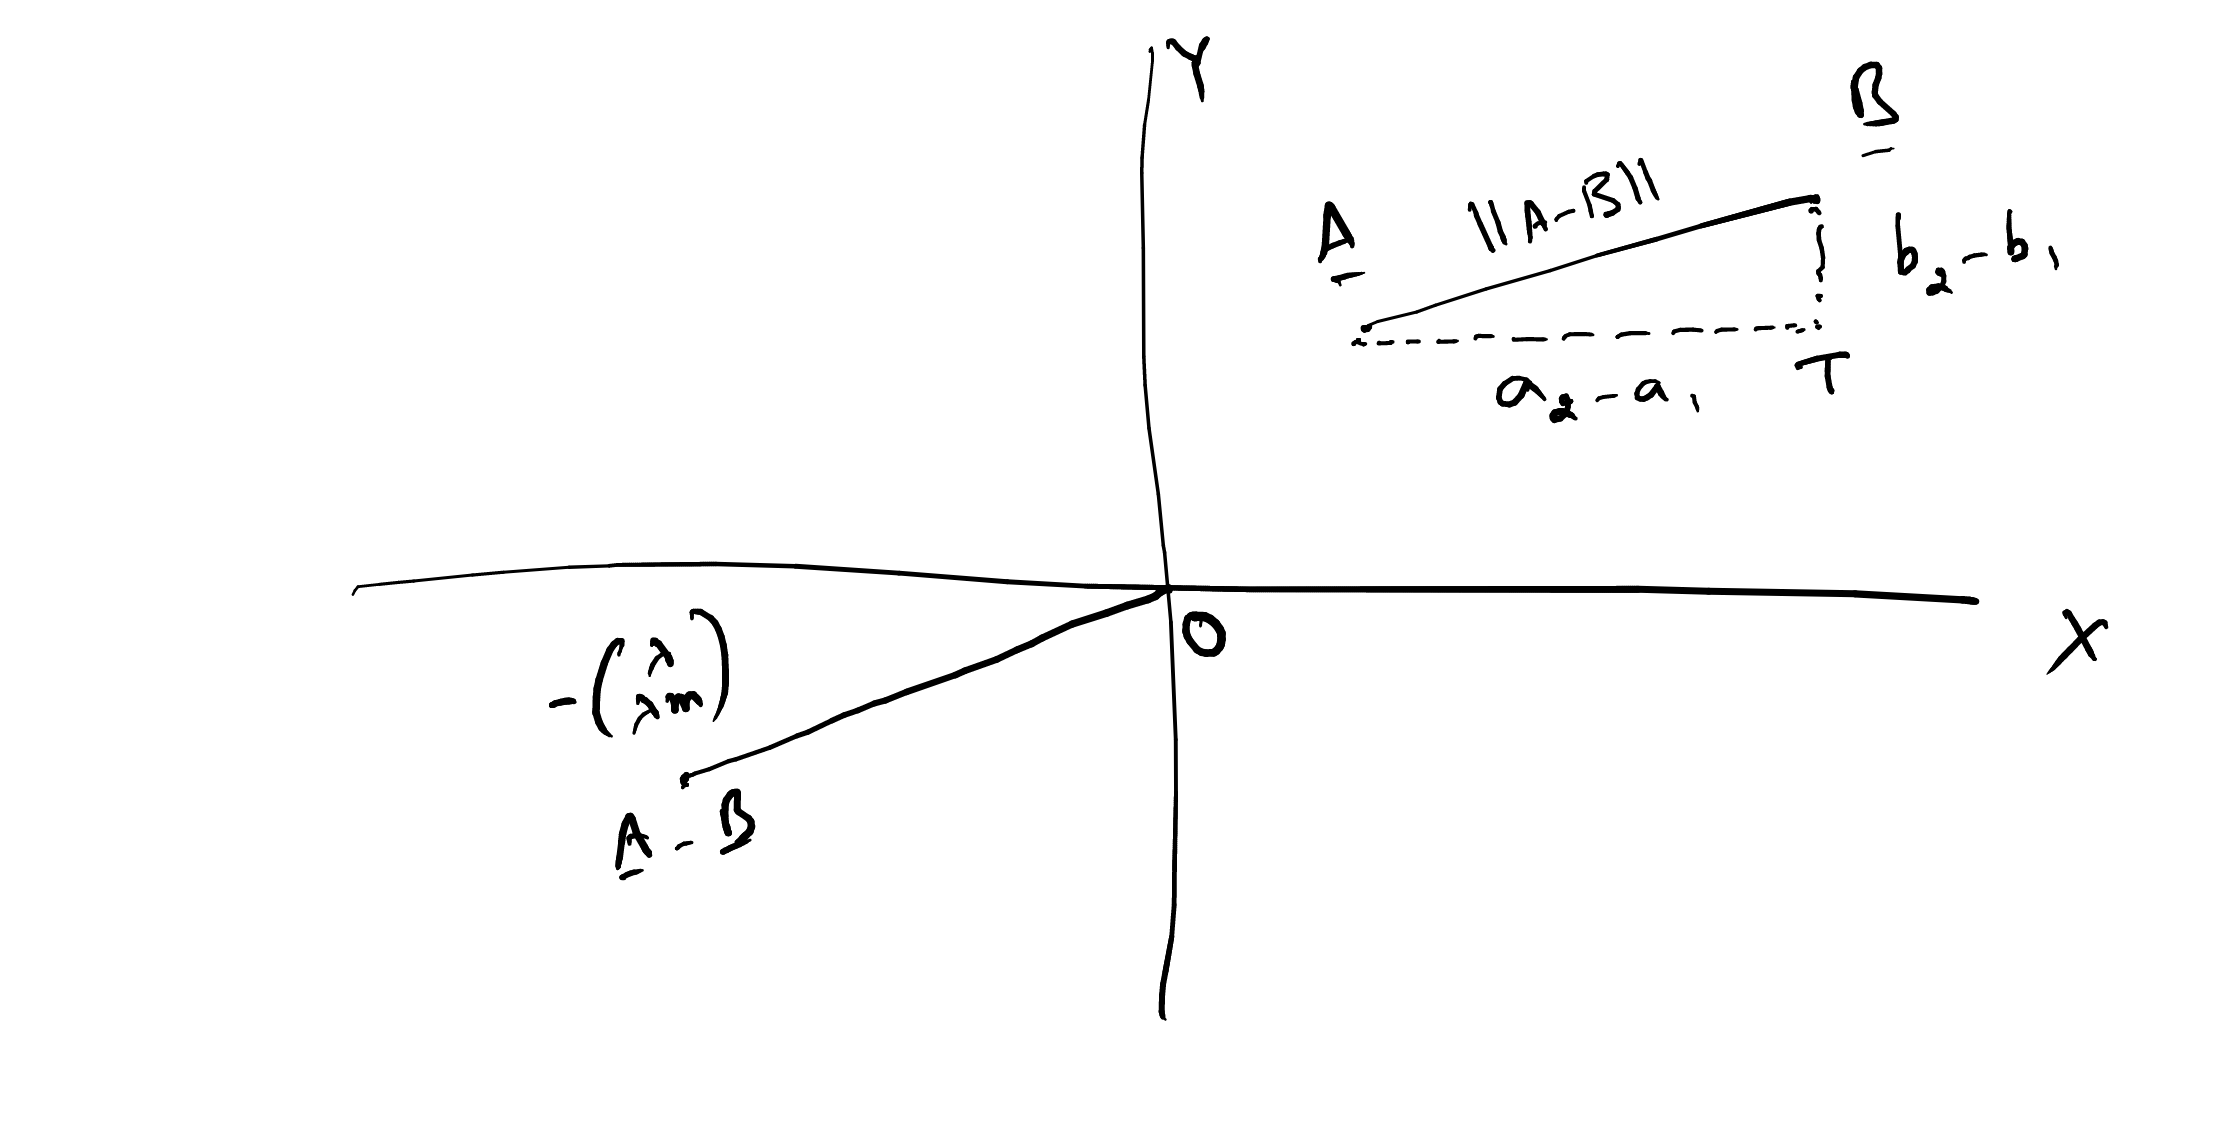
\includegraphics[width=\columnwidth]{./figs/ab.eps}
\caption{}
\label{fig:ab}
\end{figure}
%
\\
\solution See Fig. \ref{fig:ab}. From \eqref{eq:nhomog}, for some 
$\lambda$,
\begin{align}
\vec{B} &=\vec{A} + \lambda \myvec{1 \\ m}
\\
\implies \vec{A} - \vec{B} &= - \lambda \myvec{1 \\ m},
\end{align}
%
$\vec{A} - \vec{B}$ is marked in Fig. \ref{fig:ab}.
%
\item Show that $AB = \norm{\vec{A}-\vec{B}}$
\item Show that the equation of $AB$ is
\begin{align}
\label{eq:line_ab}
\vec{x} = \vec{A}+ \lambda\brak{\vec{B}-\vec{A}}
\end{align}
%
\item The {\em normal} to the vector $\vec{m}$ is defined as
\begin{align}
\label{eq:normal}
\vec{n}^T\vec{m} = 0
\end{align}
\begin{align}
\label{eq:normal_omat}
\vec{n} = \myvec{0 & 1\\ -1 & 0}\vec{m}
\end{align}
\item From \eqref{eq:line_ab}, the equation of a line can also be expressed as
\begin{align}
\label{eq:line_ab_normal}
\vec{n}^T\vec{x} &= \vec{n}^T\vec{A}+ \lambda\vec{n}^T\brak{\vec{B}-\vec{A}}
\\
\implies \vec{n}^T\vec{x} &=c
\label{eq:line_normal}
\end{align}
\item The unit vectors on the $x$ and $y$ axis are defined as
\begin{align}
\label{eq:line_unit}
\vec{e}_1 &=\myvec{1\\0}, 
\\
\vec{e}_2 &=\myvec{0\\1}
\end{align}
\item If $a$ be the {\em intercept} of the line 
\begin{align}
\label{eq:line_intercept}
\vec{n}^T\vec{x} &=c
\end{align}
on the $x-$axis, then $\myvec{a\\0}$  is a point on the line.  Thus, 
\begin{align}
%\label{eq:line_intercept}
\vec{n}^T\myvec{a\\0} &=c
\\
\implies a &= \frac{c}{\vec{n}^T\vec{e}_1}
\end{align}
%
\renewcommand{\theequation}{\theenumi}
%
\item The {\em rotation matrix} is defined as
\begin{align}
\vec{Q} = \myvec{\cos \theta & -\sin \theta\\ \sin \theta & \cos \theta}
\end{align}
%
where $\theta$ is anti-clockwise.
\item 
\begin{align}
\vec{Q}^T\vec{Q} = \myvec{1 & 0 \\ 0 & 1} = \vec{I}
\end{align}
%
where $\vec{I}$ is the {\em identity matrix}. The rotation matrix $\vec{Q}$ is also an {\em orthogonal matrix}.

\numberwithin{equation}{enumi}
%
\item Find the equation of  line $L$ in Fig. \ref{fig:line_dist}.
\\
\solution The equation of the $x-$axis is
\begin{align}
\vec{x} =\lambda \vec{e}_1
\end{align}
Translation by $p$ units along the $y-$axis results in 
\begin{align}
L_0: \quad \vec{x} = \lambda \vec{e}_1 + p \vec{e}_2 
\end{align}
Rotation by $90\degree-\alpha$ in the anti-clockwise direction yields
\begin{align}
L: \quad \vec{x} &= \vec{Q}\cbrak{\lambda \vec{e}_1 + p \vec{e}_2 }
\\
&=\lambda \vec{Q}\vec{e}_1 + p \vec{Q}\vec{e}_2 
\label{eq:line_dist_temp}
\end{align}
%
where 
\begin{align}
\vec{Q} &= \myvec{\cos \brak{\alpha-90} & -\sin \brak{\alpha-90}\\ \sin \brak{\alpha-90} & \cos \brak{\alpha-90}}
\\
&= \myvec{\sin \alpha & \cos \alpha \\ -\cos \alpha & \sin \alpha}
\end{align}
%
From \eqref{eq:line_dist_temp},
\begin{align}
L: \quad \vec{e}_2^T\vec{Q}^T\vec{x}&=\lambda \vec{e}_2^T\vec{Q}^T\vec{Q}\vec{e}_1 + p \vec{e}_2^T\vec{Q}^T\vec{Q}\vec{e}_2 
\nonumber \\
&=\lambda \vec{e}_2^T\vec{e}_1 + p \vec{e}_2^T\vec{e}_2 
\end{align}
resulting in 
\begin{align}
L: \quad \myvec{\cos \alpha & \sin \alpha}\vec{x}=p
\label{eq:line_dist_temp_final}
\end{align}
\begin{figure}
\centering
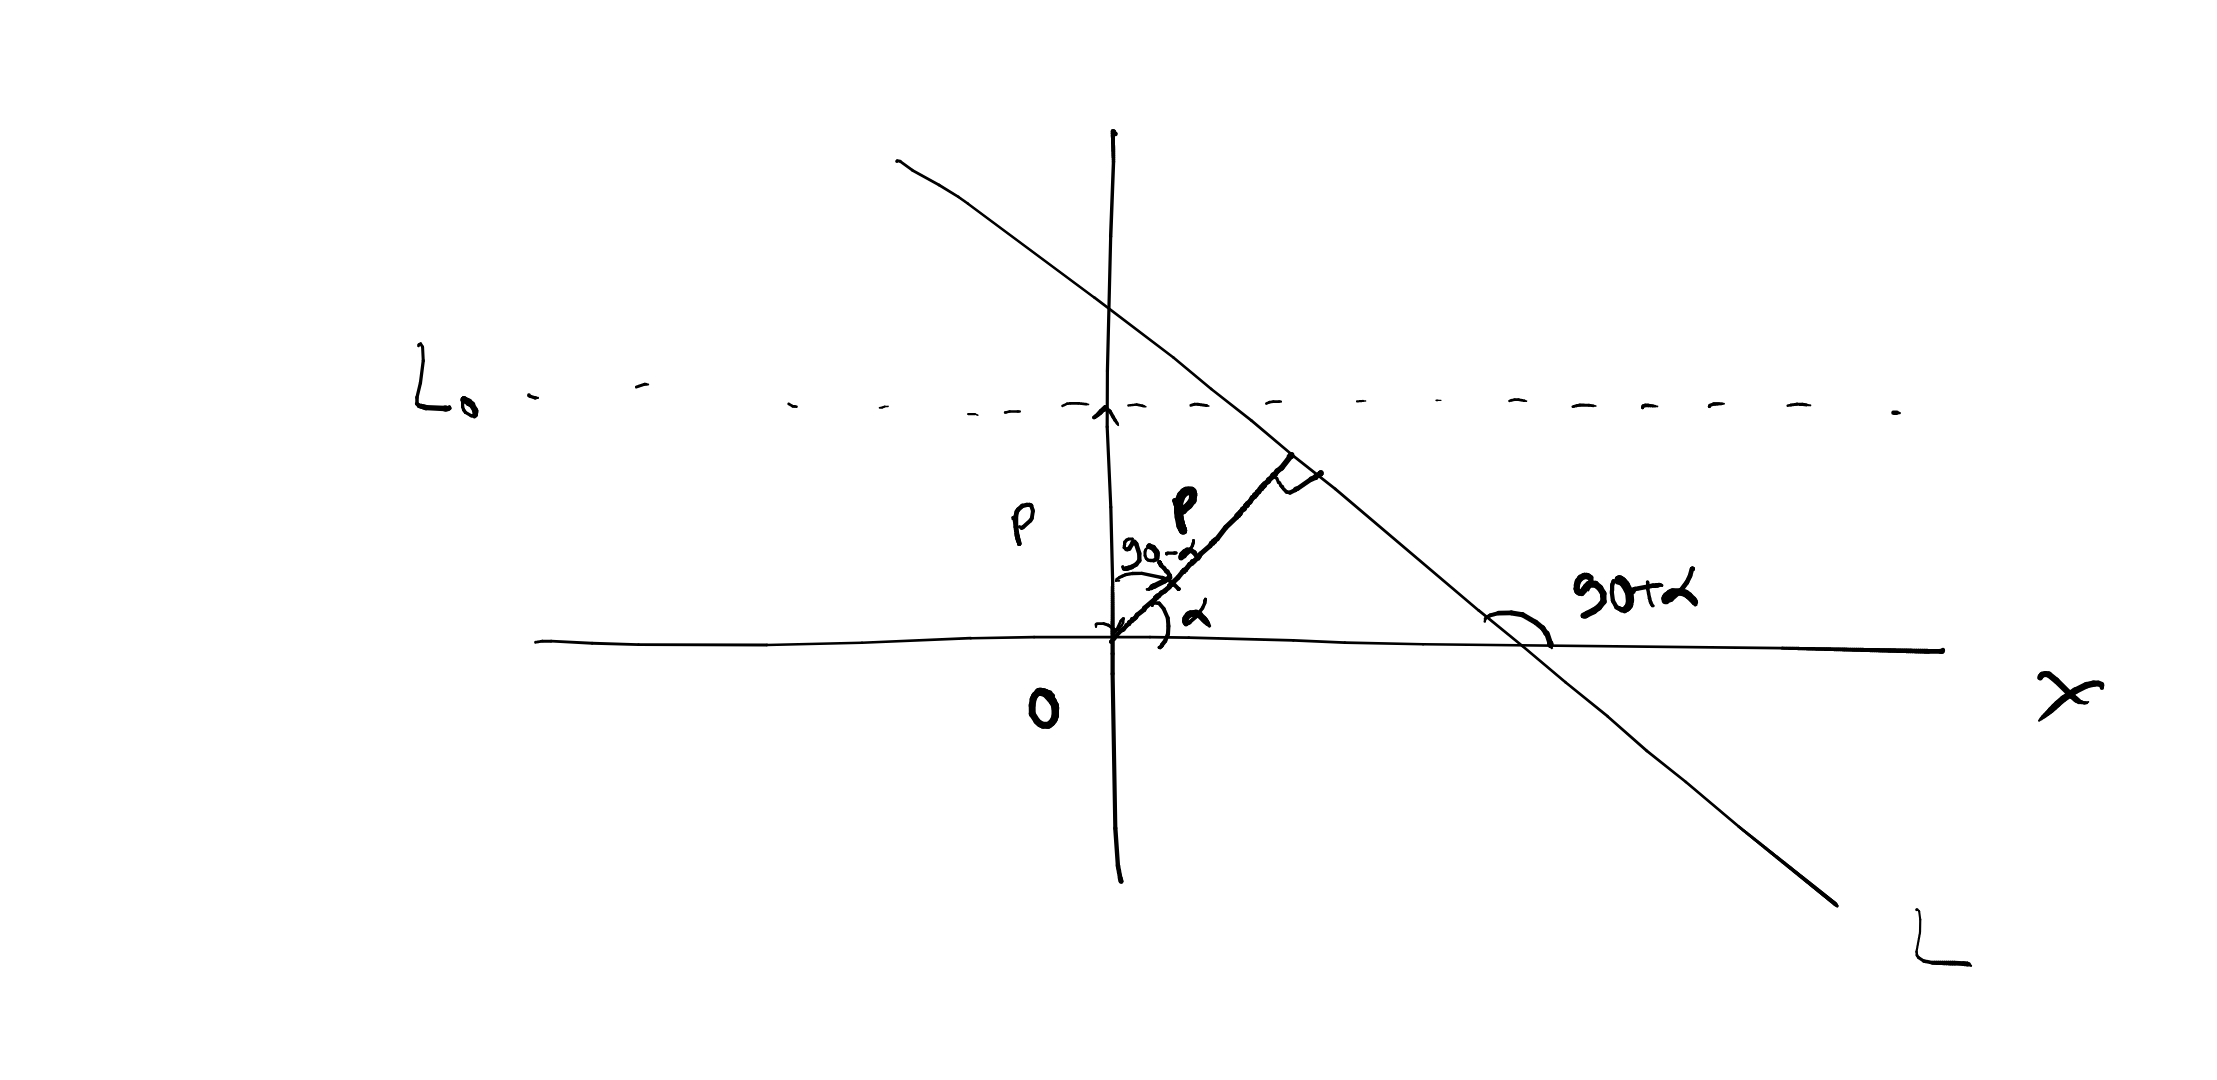
\includegraphics[width=\columnwidth]{./figs/line_dist.eps}
\caption{}
\label{fig:line_dist}
\end{figure}
\item Show that the distance from the orgin to the line 
\begin{align}
\vec{n}^T\vec{x} &=c
\end{align}
is 
\begin{align}
p = \frac{c}{\norm{n}}
\label{eq:line_dist_orig}
\end{align}
\item Show that the point of intersection of two lines 
\begin{align}
\vec{n}_1^T\vec{x} &=c_1
\\
\vec{n}_2^T\vec{x} &=c_2
\end{align}
is given by 
\begin{align}
\vec{x} &=\brak{\vec{N}^T}^{-1}\vec{c}
\end{align}
where 
\begin{align}
\vec{N} = \myvec{\vec{n}_1 & \vec{n}_2}
\end{align}
\item The {\em angle between two lines} is given by 
\begin{align}
\cos ^{-1} \frac{\vec{n}_1 ^T \vec{n}_2}{\norm{\vec{n}_1}  \norm{\vec{n}_2}}
\end{align}
\item Show that the distance of a point $\vec{x}_0$ from the line 
\begin{align}
L: \quad \vec{n}^T\vec{x} &=c
\end{align}
is 
\begin{align}
\frac{\abs{\vec{n}^T\vec{x}_0-c}}{\norm{\vec{n}}} 
\end{align}
\solution Let the equation of the line be 
\begin{align}
\vec{x} = \vec{A} + \lambda \vec{m}
\end{align}
%
where 
\begin{align}
\label{eq:line_dist_orig_pt}
\vec{n}^T\vec{A} = 0, \vec{n}^T\vec{m} = 0
\end{align}
If $\vec{x}_0$ is translated to the origin, the equation of the line $L$ becomes 
\begin{align}
\vec{x} &= \vec{A}- \vec{x}_0+ \lambda \vec{m}
\\
\implies 
\vec{n}^T\vec{x} &=c-\vec{n}^T\vec{x}_0
\end{align}
From \eqref{eq:line_dist_orig}, \eqref{eq:line_dist_orig_pt} is obtained.
\item Show that 
\begin{align}
ax^2+2bxy+cy^2+2dx+2ey+f=0
\end{align}
can be expressed as
\begin{align}
\label{eq:quad_form}
\vec{x}^T\vec{V}\vec{x}+2\vec{u}^T\vec{x}+f=0
\end{align}
%
where
\begin{align}
\vec{V} &= \vec{V}^T
\\
\vec{u} &= \myvec{d & e}
\end{align}

\item {\em Pair of straight lines:} \eqref{eq:quad_form}
%The equation
%\begin{align}
%\vec{x}^T\myvec{a & b\\ b & c}\vec{x}+2\myvec{d & e}+f=0
%\end{align}
%
represents a pair of straight lines if 
\begin{align}
\begin{vmatrix}
\vec{V}&\vec{u}
\\
\vec{u}^T&f
\end{vmatrix}
= 0
\end{align}
%
Two intersecting lines are obtained if 
\begin{align}
\abs{\vec{V}} < 0
\end{align}
\item  In Fig. \ref{fig:ratio}, let
\begin{equation}
\frac{AB}{BC} = \frac{\norm{\vec{A}-\vec{B}}}{\norm{\vec{B}-\vec{C}}} = k.
\label{eq:k}
\end{equation}
%
Show that
\begin{equation}
\frac{\vec{A}+k\vec{C}}{k+1} = \vec{B}.
\label{eq:ratio}
\end{equation}
%
\solution
%
\begin{figure}[!hb]
\centering
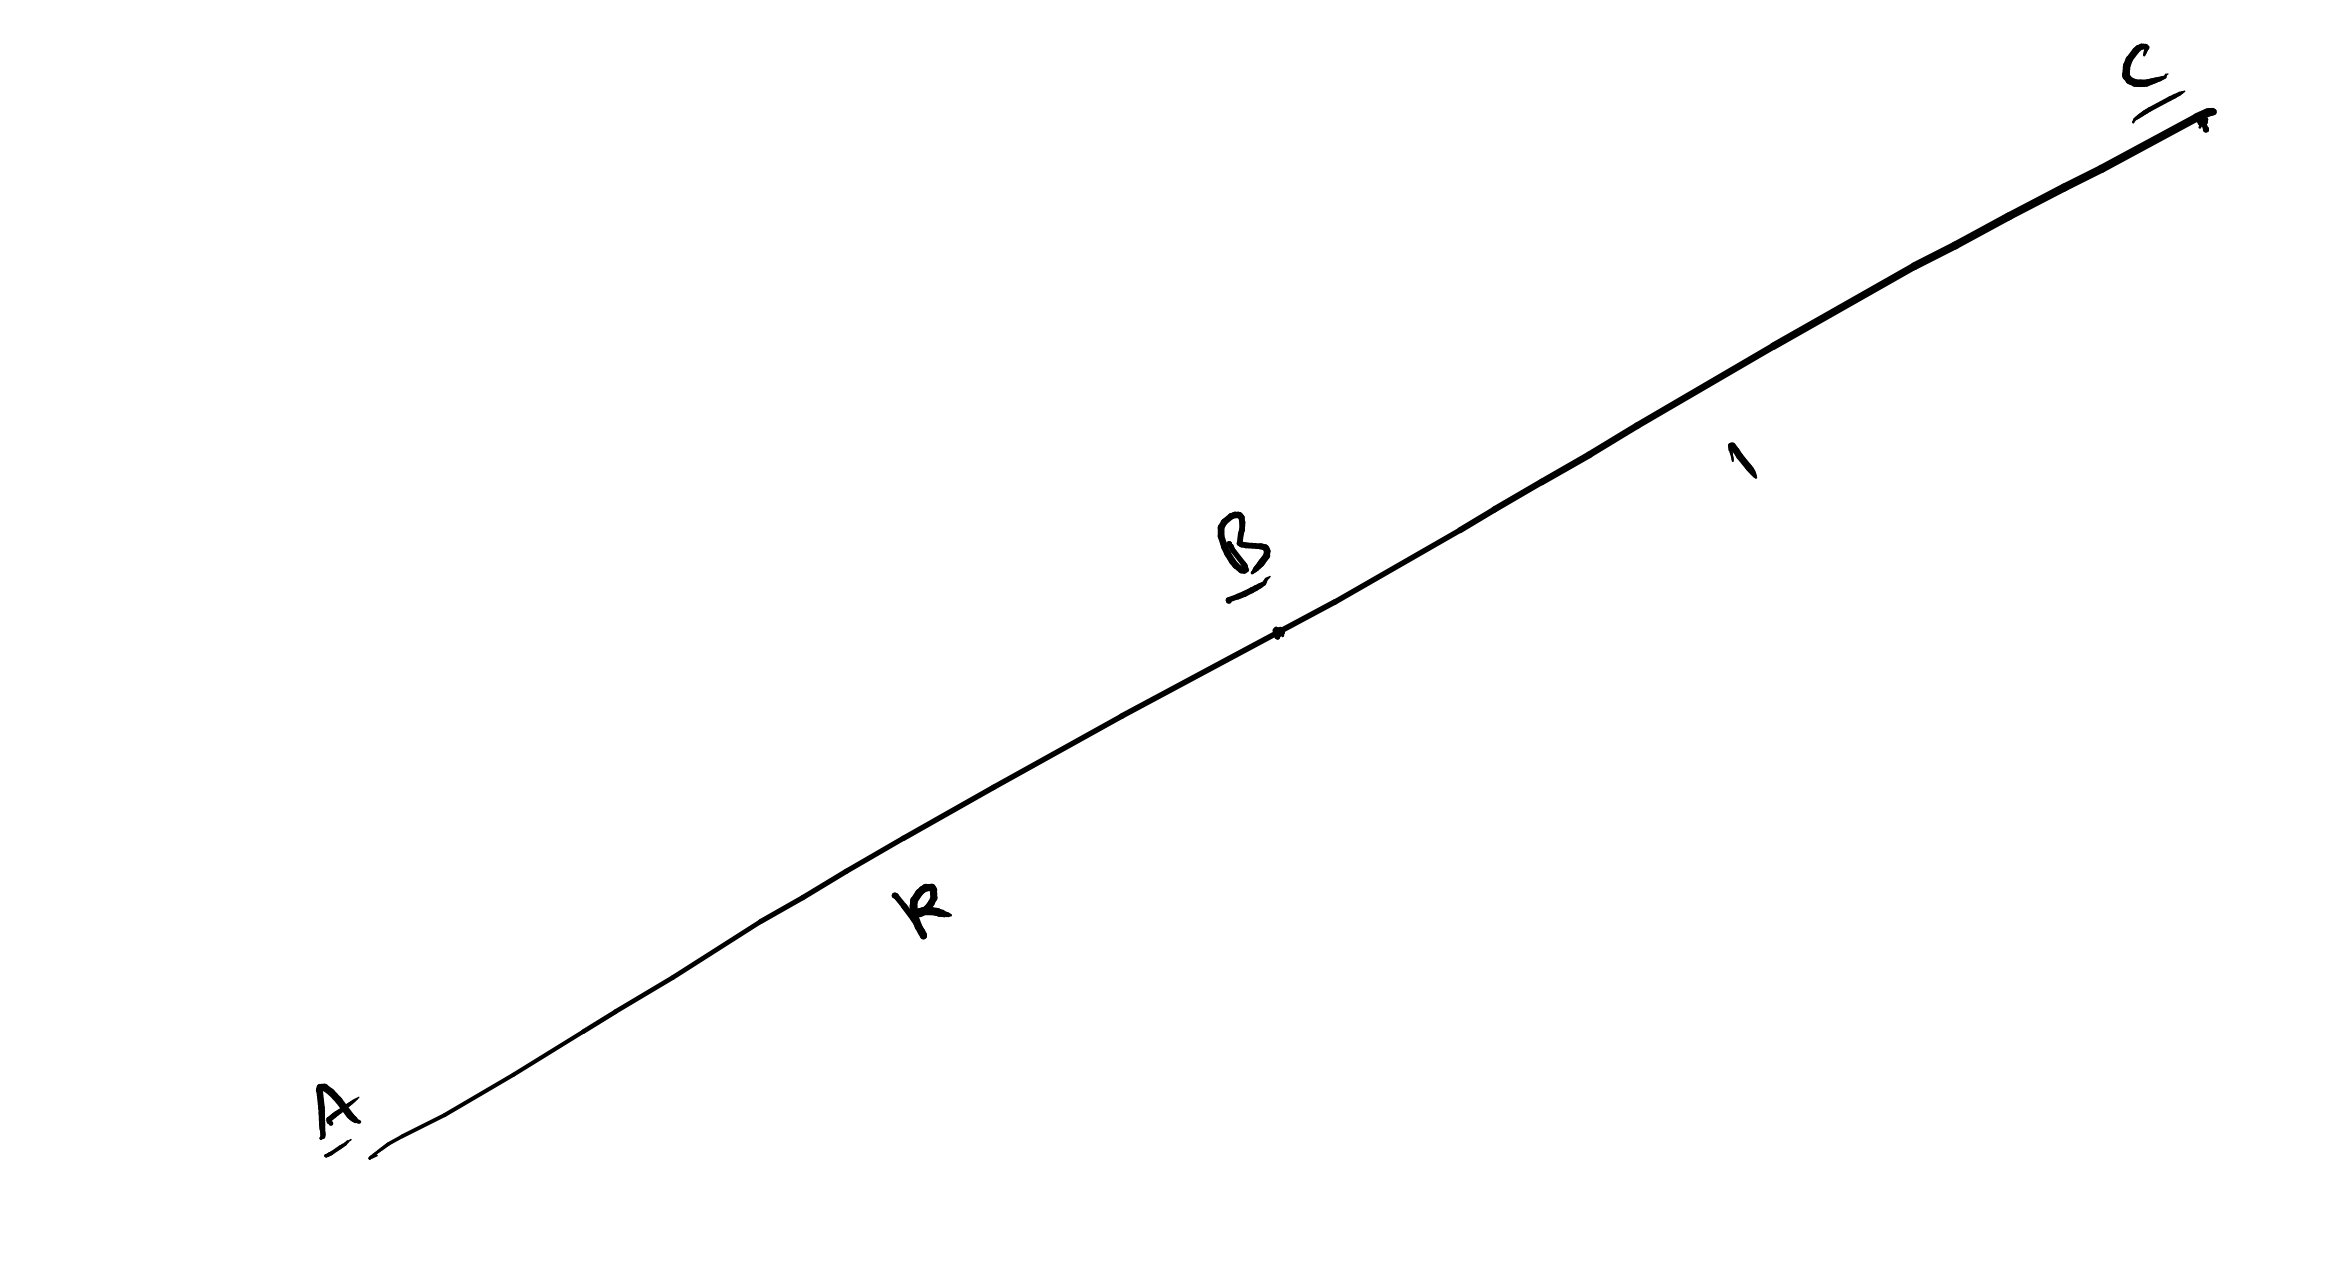
\includegraphics[width=\columnwidth]{./figs/ratio.eps}
\caption{}
\label{fig:ratio}
\end{figure}
From \eqref{eq:nhomog}, 
\begin{align}
\begin{split}
\vec{B} &= \vec{A} + \lambda_1 \vec{m}
\\
\vec{B} &= \vec{C} - \lambda_2 \vec{m}
\end{split}
\\
\label{eq:rat_1}
\implies \frac{\norm{\vec{A}-\vec{B}}}{\norm{\vec{B}-\vec{C}}} &= 
\frac{\lambda_1}{\lambda_2} = k
\\
\text{and } \frac{\vec{B}- \vec{A}}{\lambda_1} &= \frac{\vec{C}- 
\vec{B}}{\lambda_2} = \vec{m},
\label{eq:rat_2}
\end{align}
%
from \eqref{eq:k}. Using \eqref{eq:rat_1} and \eqref{eq:rat_2},
\begin{align}
\vec{A}- \vec{B} &=  k\brak{\vec{B}- \vec{C}}
\end{align}
%
resulting in \eqref{eq:ratio}

%
\item If $\vec{A}$ and $\vec{B}$ are linearly independent,  
\begin{equation}
k_1\vec{A} + k_2\vec{B} = 0 \implies k_1=k_2=0
\end{equation}
\item Show that $\vec{D}$ lies inside $\triangle ABC$ iff
\begin{align}
\vec{D} = \lambda_1\vec{A} + \lambda_2\vec{B} + \lambda_3\vec{C}
\end{align}
such that
\begin{align}
0 \le \lambda_1, \lambda_2, \lambda_3 &\le 1,
\\
0 \le \lambda_1+\lambda_2+\lambda_3 &\le 1,
\end{align}
\item Show that the equation of the angle bisectors of the lines
\begin{align}
\vec{n}_1^T\vec{x} &=c_1
\\
\vec{n}_2^T\vec{x} &=c_2
\end{align}
%
is
\begin{align}
\frac{\vec{n}_1^T\vec{x}-c_1}{\norm{\vec{n}_1}}=\pm\frac{\vec{n}_2^T\vec{x} -c_2}{\norm{\vec{n}_2}}\end{align}
%\item Show that if 
%\begin{align}
%\vec{m}_1 + k\vec{m}_2 \ne 0,
%\end{align}
%%
%there exists $k$ such that for any point $\vec{m}$,
%\begin{align}
%\label{eq:line_basis}
%\vec{m} = \vec{m}_1 + k\vec{m}_2 
%\end{align}
\item Find the equation of a line passing through the intersection of the lines
\begin{align}
\label{eq:line1}
\vec{n}_1^T\vec{x} &=c_1
\\
\vec{n}_2^T\vec{x} &=c_2
\label{eq:line2}
\end{align}
and passing through the point $\vec{p}$.
\\
\solution 
%Let the equation of any line through the intersection of \eqref{eq:line1} and \eqref{eq:line2} be 
%\begin{align}
%\vec{n}^T\vec{x} &=c
%\label{eq:line12}
%\end{align}
%
%If $\vec{u}$ be the point of intersection, 
%\begin{align}
%\myvec{\vec{n}_1^T\\ \vec{n}_2^T\\ \vec{n}^T}\vec{u} &= \myvec{c_1\\c_2\\c}
%\\
%\implies \myvec{\vec{n}_1^T & c_1\\ \vec{n}_2^T & c_2\\ \vec{n}^T & c}&
%\label{eq:line12_mat}
%\end{align}
%has rank 2.  Thus, 
%%
%\begin{align}
%\label{eq:line_basis_normal}
%\myvec{\vec{n}\\c} &= k_1\myvec{\vec{n}_1 \\ c_1}+ k_2\myvec{\vec{n}_2\\c_2} 
%\end{align}
%Substituting in \eqref{eq:line12},
%\begin{align}
%\vec{n}^T\vec{x} = c &
%\implies \vec{n}_1^T\vec{x} + k\vec{n}_2^T\vec{x} =  c_1+kc_2=c
%\label{eq:line_basis_normal_temp}
%\end{align}
%%
%Thus, 
%\begin{align}
%k = \frac{\vec{n}_1^T\vec{p}-c_1}{\vec{n}_2^T\vec{p}-c_2}
%\end{align}
%%
%which can be used to obtain the desired equation using \eqref{eq:line_basis_normal_temp}
%
%Alternatively, 
%
%
The intersection of the lines is 
\begin{align}
\vec{x} = \vec{N}^{-T}\vec{c}
\end{align}
%
where 
\begin{align}
\vec{N} &= \myvec{\vec{n}_1 &\vec{n}_2}
\\
\vec{c} &= \myvec{c_1 \\ c_2} 
\end{align}
Thus, the equation of the desired line is 
\begin{align}
\vec{x} = \vec{p}+ \lambda\brak{\vec{N}^{-T}\vec{c}-\vec{p}}&
\\
\implies \vec{N}^{T}\vec{x} = \vec{N}^{T}\vec{p}+ \lambda\brak{\vec{c}-\vec{N}^{T}\vec{p}}&
\end{align}
resulting in 
\begin{multline}
 \brak{\vec{c}-\vec{N}^T\vec{p}}^T\myvec{0 & -1 \\ 1 & 0}\vec{N}^T\vec{x} 
\\
= \brak{\vec{c}-\vec{N}^T\vec{p}}^T\myvec{0 & -1 \\ 1 & 0}\vec{N}^T\vec{p}
\end{multline}
\item Find $\vec{R}$, the {\em reflection}  of $\vec{P}$ about the line
\begin{align}
L: \quad \vec{n}^T\vec{x} = c
\end{align}
%
\begin{figure}
\centering
\includegraphics[width=\columnwidth]{./figs/reflection.eps}
\caption{}
\label{fig:locus}
\end{figure}
\solution Since $\vec{R}$ is the reflection of $\vec{P}$ and $\vec{Q}$ lies on $L$, $\vec{Q}$ bisects $PR$.  
This leads to the following equations
Hence, 
\begin{align}
\label{eq:reflect_bisect}
2\vec{Q} &= \vec{P}+\vec{R}
\\
\label{eq:reflect_Q}
\vec{n}^{T}\vec{Q} &= c
\\
\label{eq:reflect_R}
\vec{m}^{T}\vec{R} &= \vec{m}^{T}\vec{P}
\end{align}
%
where $\vec{m}$ is the direction vector of $L$.  From \eqref{eq:reflect_bisect} and \eqref{eq:reflect_Q},
\begin{align}
\label{eq:reflect_bisectQ}
\vec{n}^{T}\vec{R}  &= 2c - \vec{n}^{T}\vec{P}
\end{align}
%
From \eqref{eq:reflect_bisectQ} and \eqref{eq:reflect_R},
\begin{align}
\label{eq:reflect_bisectQR}
\myvec{\vec{m} & \vec{n}}^T\vec{R} &= \myvec{\vec{m} & -\vec{n}}^T\vec{P}+ \myvec{0 \\ 2c}
\end{align}
%
Letting 
\begin{align}
\label{eq:reflect_mat}
\vec{V}=  \myvec{\vec{m} & \vec{n}}
\end{align}
with the condition that $\vec{m},\vec{n}$ are orthonormal, i.e.
\begin{align}
\label{eq:reflect_ortho}
\vec{V}^T\vec{V}=  \vec{I}
\end{align}
%
Noting that 
\begin{align}
\label{eq:reflect_trans}
\myvec{\vec{m} & -\vec{n}} &= \myvec{\vec{m} & \vec{n}} \myvec{1 & 0 \\ 0 & -1},
\end{align}
\eqref{eq:reflect_bisectQR} can be expressed as
%
\begin{align}
\label{eq:reflect_}
\vec{V}^T\vec{R} &=  \sbrak{\vec{V}\myvec{1 & 0 \\ 0 & -1}}^T\vec{P}+\myvec{0 \\ 2c}
\\
\implies \vec{R} &= \sbrak{\vec{V}\myvec{1 & 0 \\ 0 & -1}\vec{V}^{-1}}^T\vec{P}+ \vec{V}\myvec{0 \\ 2c}
\\
 &=\vec{V}\myvec{1 & 0 \\ 0 & -1}\vec{V}^T \vec{P}+2c \vec{n}
\end{align}
\item Show that, for any $\vec{m},\vec{n}$, the reflection is also given by
\begin{align}
%\label{eq:reflect_bisect}
\frac{\vec{R}}{2} = \frac{\vec{m}\vec{m}^T-\vec{n}\vec{n}^T}{\vec{m}^T\vec{m}+\vec{n}^T\vec{n}}\vec{P} + c 
\frac{\vec{n}}{\norm{\vec{n}}^2}
\end{align}

\end{enumerate}
%
%
%\item Let $\vec{x}$ be any point on $AB$ in Fi.g \ref{fig:orth}.  Show that
%\begin{equation}
%\brak{\vec{x}-\vec{A}}^T\brak{\vec{B}-\vec{C}} = 0
%\end{equation}
%%
%\item If $\vec{x,y}$ are any two points on $AB$, show that 
%\begin{equation}
%\label{eq:orth_any}
%\brak{\vec{x}-\vec{y}}^T\brak{\vec{B}-\vec{C}} = 0
%\end{equation}
%%
%\item In Fig. \ref{fig:alt}, $BE \perp AC, CF \perp AB$.  Show that $AD \perp BC$.
%\begin{figure}[!hb]
%\centering
%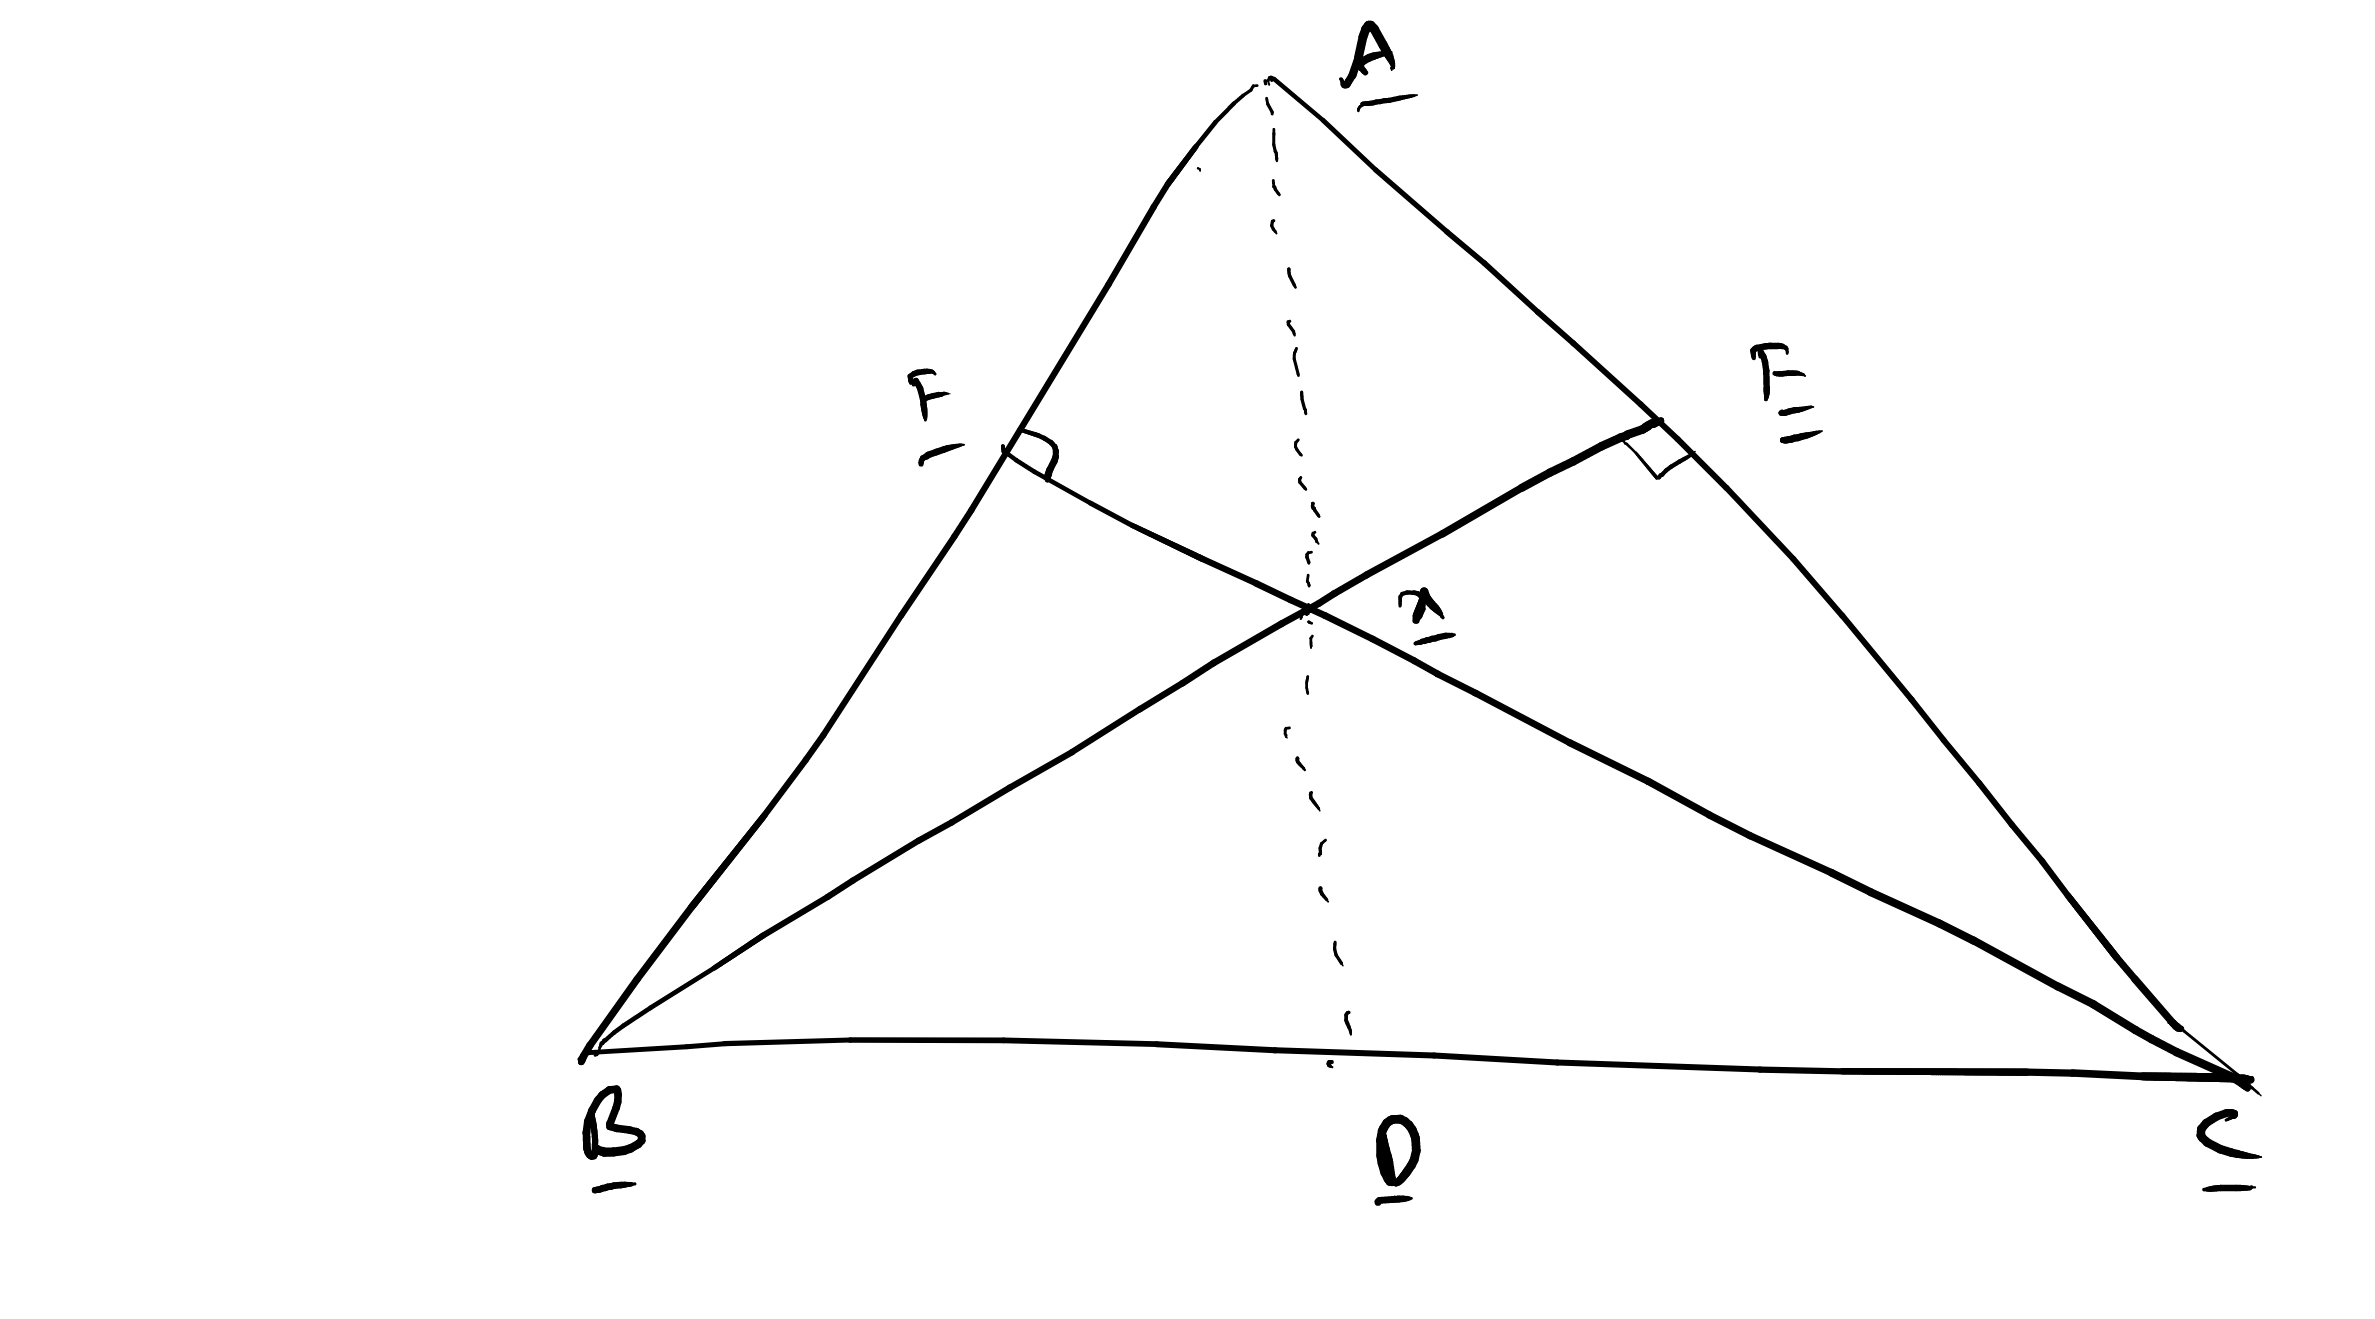
\includegraphics[width=\columnwidth]{./figs/alt.eps}
%\caption{}
%\label{fig:alt}
%\end{figure}
%\\
%\solution Let $\vec{x}$ be the intersection of $BE$ and $CF$. Then, using 
%\eqref{eq:orth_any},
%\begin{align}
%\label{eq:alt_1}
%\begin{split}
%\brak{\vec{x}-\vec{B}}^T
%\brak{\vec{A}-\vec{C}} &= 0
%\\
%\brak{\vec{x}-\vec{C}}^T
%\brak{\vec{A}-\vec{B}} &=0
%\end{split}
%\\
%\label{eq:alt_3}
%\implies \vec{x}^T\brak{\vec{A}-\vec{C}}-\vec{B}^T\brak{\vec{A}-\vec{C}} &= 0
%\\
%\text{and }\vec{x}^T\brak{\vec{A}-\vec{B}}-\vec{C}^T\brak{\vec{A}-\vec{B}} &= 0
%\label{eq:alt_4}
%\end{align}
%%
%Subtracting \eqref{eq:alt_4} from \eqref{eq:alt_3},
%\begin{align}
%\vec{x}^T\brak{\vec{B}-\vec{C}} + \vec{A}^T\brak{\vec{C}-\vec{B}} &= 0
%\\
%\implies \brak{\vec{x}^T - \vec{A}^T}\brak{\vec{B}-\vec{C}}  &= 0
%\\
%\implies \brak{\vec{x} - \vec{A}}^T\brak{\vec{B}-\vec{C}}  &= 0
%\end{align}
%%
%which completes the proof.
%\end{enumerate}
%

\subsection{Programming}
\renewcommand{\theequation}{\theenumi}
\begin{enumerate}[label=\arabic*.,ref=\thesubsection.\theenumi]
\item Find the intercepts made on the axes by the straight lines whose equations are
\begin{multicols}{2}
\begin{enumerate}
%\begin{enumerate}[(i)]
%\setlength\itemsep{2em}
\item
$
\myvec{2 & 3}\vec{x} = 2
$
\item
$
\myvec{1 & -3}\vec{x} = -5
$ 
\item
$
\myvec{1 & -1}\vec{x} = 0
$
\item
$
\myvec{\frac{1}{a+b} & \frac{1}{a-b}}\vec{x} = \frac{1}{a^2-b^2}
$
\item 
$
\myvec{1 & -m}\vec{x} = -c
$
\end{enumerate}
\end{multicols}
\item Write down the equations of straight lines which make the following pairs of intercepts on the axes:
\begin{multicols}{2}
\begin{enumerate}
\item 3,-4
\item -5,6
\item 
$
\frac{1}{a},\frac{1}{b}
$
\item 
$
2a,-2a
$
\end{enumerate}
\end{multicols}
\item A straight line passes through a fixed point $\myvec{h\\k}$ and cuts the axes in $\vec{A},\vec{B}$.  Parallels to the
axes through $\vec{A}$ and $\vec{B}$ intersect in $\vec{P}$.  Find the equation of the locus of $\vec{P}$.
\end{enumerate}

\subsection{Example}
\begin{enumerate}[1.]
\item Find the equations of two straight lines at a distance 3 from the origin and making an angle of $120 \degree$ with $OX$.
\item Find the equation of a straight line making an angle of $60\degree$ with $OX$ and passing through the point $\brak{2,-2}$.
Transform the equation to the form
\begin{equation*}
x\cos\alpha + y\sin \alpha = p 
\end{equation*}
\item Find the equation of the straight line that passes through the points $\brak{2,3}$ and $\brak{3,2}$. What is its inclination
to $OX$?
\item Find the equation of the straight line through the point $\brak{5,7}$ that makes equal intercepts on the axes.
\item Find the equations of the sides of a triangle whose corners are $\brak{2,4}$, $\brak{-4,1}$ and $\brak{2,-3}$.
\item For the same triangle find the equations of the lines joining the corners to the middle points of the opposite sides.
\item Find the equation of a straight line passing through the point $\brak{2,-3}$ parallel to the line $4x-y+7=0$.
\item Find the intercepts on the axes made by a straight line which passes through the point $\brak{3,-1}$ and makes an angle
of $30\degree$ with $OX$.
\item Find the equation of the straight line through the points $\brak{3,-4}$, $\brak{2,3}$ and of the
parallel line through $\brak{5,2}$.
\item What is the distance from the origin of the line $4x-y-7$? Write down the equation of a parallel line at double the distance.
\item Find the equation of the straight line through the point $\brak{3,-4}$ parallel to the line joining the origin to the point
$\brak{2,-1}$.
\item Write down the equation of the straight line which makes intercepts 2 and -7 on the axes, and of the parallel line through
the point $\brak{3,-1}$.
\item Find the equations of the straight line joining the points $\brak{3,4}$, $\brak{-2,1}$ and of the parallel line through
the origin.
\item $ABC$ is a triangle and $A, B$ and $C$ are the points $\brak{2,3}$, $\brak{5,-1}$ and $\brak{-4,2}$.  Find the equation
of the straight line through $A$ parallel to $BC$.
\item Find the equation of a line parallel to $2x+5y=11$ passing through the middle point of the join of the points $\brak{-7,3}$, $\brak{5,-11}$.
\item The base of a triangle passes through a fixed point $\brak{f,g}$ and the sides are bisected at right angles by the axes.  Prove that the locus
of the vertex is the line
\begin{equation*}
gx+fy = 0
\end{equation*}
\end{enumerate}

\subsection{Exercises}
\renewcommand{\theequation}{\theenumi}
\begin{enumerate}[label=\arabic*.,ref=\thesubsection.\theenumi]
\item Find the vertices of the triangle whose sides are
\numberwithin{equation}{enumi}
\begin{align}
\myvec{3 & 2}\vec{x}+6 &= 0,
\\
 \myvec{2 & -5}\vec{x}+4 &= 0,
\\
 \myvec{1 & -3}\vec{x} -6 &= 0
\end{align}
\item Prove that the lines
\begin{align}
\myvec{1 & 1}\vec{x}+25 &= 0, 
\\
\myvec{2 & 3}\vec{x}+7 &= 0 
\\
\myvec{3 & 5}\vec{x} = 11
\end{align}
%
are concurrent, and find the coordinates of their common point.
\item Find the equation of a line parallel to the line 
\begin{align}
\myvec{2 & -1}\vec{x}=3
\end{align}
 and passing through the intersection of the lines
\begin{align}
\myvec{3 & 1}\vec{x}&=7
\\
 \myvec{2 & -3}\vec{x} &= 5
\end{align}
\item Find the equation of the line joining the origin to the point of intersection of the lines
\begin{align}
\myvec{3&-5}\vec{x} &= 11
\\
 \myvec{2&7}\vec{x}+4 &= 0
\end{align}
%
\item Find the acute angle between the lines
\numberwithin{equation}{enumi}
\begin{align}
\myvec{1 & -1} \vec{x}=  - 7 
\\
 \myvec{2+\sqrt{3}& 1} \vec{x}= 11
\end{align}
\item Find the angle between the lines
\begin{align}
\myvec{-2 & 1} \vec{x}&= 5 
\\
 \myvec{2 & 4} \vec{x}+ 11 &= 0
\end{align}
\renewcommand{\theequation}{\theenumi}
\item Find the equation of a straight line through the point $\myvec{2\\-4}$ at right angles to the line 
\begin{align}
\myvec{5 & 7}\vec{x}+12=0
\end{align}
 and find the point in
which the lines intersect.
\item Find the equation of a straight line through the origin and at right angles to the line
\begin{align}
\myvec{a &b} \vec{x}+c= 0
\end{align}
\item Find the equation of a straight line at right angles to the line
\numberwithin{equation}{enumi}
\begin{align}
\myvec{5 &-2}\vec{x}+11 = 0
\end{align}
and passing through the intersecton of the lines
\begin{align}
\myvec{1 & 2}\vec{x}+1 &= 0,
\\
 \myvec{-1 & 1} \vec{x}&= 7. 
\end{align}
\item The origin is a corner of a square and two of its sides have equations
\begin{align}
\myvec{2 & 1} \vec{x}&= 0
\\
 \myvec{2 & 1}\vec{x}&= 3.
\end{align}
Find the equations of the other two sides.
\item Write down the equations of the perpendiculars from the origin to the lines
\begin{align}
\myvec{1 & 5} \vec{x}&= 13, 
\\
\myvec{5 & 1} \vec{x}&= 13
\end{align}
and find the equation of the line joining the feet of the perpendiculars.
\item Prove that the line 
\begin{align}
\myvec{1 & 1} \vec{x}= 11
\end{align}
 makes equal angles with the lines
\begin{align}
\myvec{1 & -\brak{2-\sqrt{3}}}\vec{x} + 2 &= 0,
\\
 \myvec{\brak{2-\sqrt{3}} &  - 1}\vec{x} + 5 &= 0
\end{align}
\renewcommand{\theequation}{\theenumi}
\item $\vec{A}$ is the point $\myvec{-4\\0}$ and $\vec{B}$ is the point $\myvec{3\\0}$.  Find the locus of a point $\vec{P}$ such that the angles $APO$, $OPB$ are equal, where $\vec{O}$ is the origin.
\end{enumerate}
 
\section{Conics}
\subsection{Definitions}
\renewcommand{\theequation}{\theenumi}
\begin{enumerate}[label=\arabic*.,ref=\thesubsection.\theenumi]
\item The equation of a quadratic curve is given by
%\begin{equation}
%Ax_1^2+Bx_1x_2+Cx_2^2+Dx_1+Ex_2+F = 0
%\label{eq:quadratic}
%\end{equation}
%
%Show that  \eqref{eq:quadratic} can be expressed as
\begin{equation}
\vec{x}^T\vec{V}\vec{x}+2\vec{u}^T\vec{x}+ f = 0
\label{eq:quadratic_vec}
\end{equation}
%
%Find the matrix $\vec{V}$ and vector $\vec{u}$.
\item Show that 
\begin{align}
\frac{d\brak{\vec{u}^T\vec{x}}}{d\vec{x}} = \vec{u}
%+ \frac{d\vec{x}}{dx_1}V^T
%= 0
\end{align}
\item Show that 
\begin{align}
\frac{d\brak{\vec{x}^T\vec{V}\vec{x}}}{d\vec{x}} = 2\vec{V}^T\vec{x}
\end{align}
\item Show that 
\begin{align}
\frac{d\vec{x}}{dx_1} = \vec{m}
\end{align}
%
\numberwithin{equation}{enumi}
\item Find the {\em normal} vector to the curve in \eqref{eq:quadratic_vec} at 
point $\vec{p}$.
\\
\solution Differentiating \eqref{eq:quadratic_vec} with respect to 
$x_1$,
\begin{align}
\frac{d\brak{\vec{x}^T\vec{V}\vec{x}}}{d\vec{x}}\frac{d\vec{x}}{dx_1}+\frac{d\brak{\vec{u}^T\vec{x}}}{d\vec{x}}\frac{d\vec{x}}{dx_1}
&= 0
\\
\implies 2\vec{x}^T\vec{V}\vec{m}+2\vec{u}^T\vec{m}
& = 0  \because \brak{\frac{d\vec{x}}{dx_1} = \vec{m}}
\end{align}
Substituting  $\vec{x} = \vec{p}$ and simplifying
\begin{align}
\brak{ \vec{V}\vec{p}+\vec{u}}^T\vec{m} & = 0 
\\
\implies \vec{n} &= \vec{V}\vec{p}+\vec{u}
\end{align}
%
\renewcommand{\theequation}{\theenumi}
\item The {\em tangent} to the curve at $\vec{p}$ is given by 
\begin{align}
\vec{n}^T\brak{\vec{x}-\vec{p}} = 0
\end{align}
\item Let $\vec{P}$ be a rotation matrix and  $\vec{c}$ be a vector. Then 
\begin{align}
\vec{x} = \vec{P}\vec{y}+\vec{c}.
\label{eq:affine}
\end{align}
 is known as an {\em affine} transformation.
\item Classify the various conic sections based on $\eqref{eq:quadratic_vec}$.
\\
\solution 
\begin{table}[!ht]
\begin{center}
%%%%%%%%%%%%%%%%%%%%%%%%%%%%%%%%%%%%%%%%%%%%%%%%%%%%%%%%%%%%%%%%%%%%%%
%%                                                                  %%
%%  This is the header of a LaTeX2e file exported from Gnumeric.    %%
%%                                                                  %%
%%  This file can be compiled as it stands or included in another   %%
%%  LaTeX document. The table is based on the longtable package so  %%
%%  the longtable options (headers, footers...) can be set in the   %%
%%  preamble section below (see PRAMBLE).                           %%
%%                                                                  %%
%%  To include the file in another, the following two lines must be %%
%%  in the including file:                                          %%
%%        \def\inputGnumericTable{}                                 %%
%%  at the beginning of the file and:                               %%
%%        \input{name-of-this-file.tex}                             %%
%%  where the table is to be placed. Note also that the including   %%
%%  file must use the following packages for the table to be        %%
%%  rendered correctly:                                             %%
%%    \usepackage[latin1]{inputenc}                                 %%
%%    \usepackage{color}                                            %%
%%    \usepackage{array}                                            %%
%%    \usepackage{longtable}                                        %%
%%    \usepackage{calc}                                             %%
%%    \usepackage{multirow}                                         %%
%%    \usepackage{hhline}                                           %%
%%    \usepackage{ifthen}                                           %%
%%  optionally (for landscape tables embedded in another document): %%
%%    \usepackage{lscape}                                           %%
%%                                                                  %%
%%%%%%%%%%%%%%%%%%%%%%%%%%%%%%%%%%%%%%%%%%%%%%%%%%%%%%%%%%%%%%%%%%%%%%



%%  This section checks if we are begin input into another file or  %%
%%  the file will be compiled alone. First use a macro taken from   %%
%%  the TeXbook ex 7.7 (suggestion of Han-Wen Nienhuys).            %%
\def\ifundefined#1{\expandafter\ifx\csname#1\endcsname\relax}


%%  Check for the \def token for inputed files. If it is not        %%
%%  defined, the file will be processed as a standalone and the     %%
%%  preamble will be used.                                          %%
\ifundefined{inputGnumericTable}

%%  We must be able to close or not the document at the end.        %%
	\def\gnumericTableEnd{\end{document}}


%%%%%%%%%%%%%%%%%%%%%%%%%%%%%%%%%%%%%%%%%%%%%%%%%%%%%%%%%%%%%%%%%%%%%%
%%                                                                  %%
%%  This is the PREAMBLE. Change these values to get the right      %%
%%  paper size and other niceties.                                  %%
%%                                                                  %%
%%%%%%%%%%%%%%%%%%%%%%%%%%%%%%%%%%%%%%%%%%%%%%%%%%%%%%%%%%%%%%%%%%%%%%

	\documentclass[12pt%
			  %,landscape%
                    ]{report}
       \usepackage[latin1]{inputenc}
       \usepackage{fullpage}
       \usepackage{color}
       \usepackage{array}
       \usepackage{longtable}
       \usepackage{calc}
       \usepackage{multirow}
       \usepackage{hhline}
       \usepackage{ifthen}

	\begin{document}


%%  End of the preamble for the standalone. The next section is for %%
%%  documents which are included into other LaTeX2e files.          %%
\else

%%  We are not a stand alone document. For a regular table, we will %%
%%  have no preamble and only define the closing to mean nothing.   %%
    \def\gnumericTableEnd{}

%%  If we want landscape mode in an embedded document, comment out  %%
%%  the line above and uncomment the two below. The table will      %%
%%  begin on a new page and run in landscape mode.                  %%
%       \def\gnumericTableEnd{\end{landscape}}
%       \begin{landscape}


%%  End of the else clause for this file being \input.              %%
\fi

%%%%%%%%%%%%%%%%%%%%%%%%%%%%%%%%%%%%%%%%%%%%%%%%%%%%%%%%%%%%%%%%%%%%%%
%%                                                                  %%
%%  The rest is the gnumeric table, except for the closing          %%
%%  statement. Changes below will alter the table's appearance.     %%
%%                                                                  %%
%%%%%%%%%%%%%%%%%%%%%%%%%%%%%%%%%%%%%%%%%%%%%%%%%%%%%%%%%%%%%%%%%%%%%%

\providecommand{\gnumericmathit}[1]{#1} 
%%  Uncomment the next line if you would like your numbers to be in %%
%%  italics if they are italizised in the gnumeric table.           %%
%\renewcommand{\gnumericmathit}[1]{\mathit{#1}}
\providecommand{\gnumericPB}[1]%
{\let\gnumericTemp=\\#1\let\\=\gnumericTemp\hspace{0pt}}
 \ifundefined{gnumericTableWidthDefined}
        \newlength{\gnumericTableWidth}
        \newlength{\gnumericTableWidthComplete}
        \newlength{\gnumericMultiRowLength}
        \global\def\gnumericTableWidthDefined{}
 \fi
%% The following setting protects this code from babel shorthands.  %%
 \ifthenelse{\isundefined{\languageshorthands}}{}{\languageshorthands{english}}
%%  The default table format retains the relative column widths of  %%
%%  gnumeric. They can easily be changed to c, r or l. In that case %%
%%  you may want to comment out the next line and uncomment the one %%
%%  thereafter                                                      %%
\providecommand\gnumbox{\makebox[0pt]}
%%\providecommand\gnumbox[1][]{\makebox}

%% to adjust positions in multirow situations                       %%
\setlength{\bigstrutjot}{\jot}
\setlength{\extrarowheight}{\doublerulesep}

%%  The \setlongtables command keeps column widths the same across  %%
%%  pages. Simply comment out next line for varying column widths.  %%
\setlongtables

\setlength\gnumericTableWidth{%
	53pt+%
	53pt+%
	53pt+%
0pt}
\def\gumericNumCols{3}
\setlength\gnumericTableWidthComplete{\gnumericTableWidth+%
         \tabcolsep*\gumericNumCols*2+\arrayrulewidth*\gumericNumCols}
\ifthenelse{\lengthtest{\gnumericTableWidthComplete > \linewidth}}%
         {\def\gnumericScale{\ratio{\linewidth-%
                        \tabcolsep*\gumericNumCols*2-%
                        \arrayrulewidth*\gumericNumCols}%
{\gnumericTableWidth}}}%
{\def\gnumericScale{1}}

%%%%%%%%%%%%%%%%%%%%%%%%%%%%%%%%%%%%%%%%%%%%%%%%%%%%%%%%%%%%%%%%%%%%%%
%%                                                                  %%
%% The following are the widths of the various columns. We are      %%
%% defining them here because then they are easier to change.       %%
%% Depending on the cell formats we may use them more than once.    %%
%%                                                                  %%
%%%%%%%%%%%%%%%%%%%%%%%%%%%%%%%%%%%%%%%%%%%%%%%%%%%%%%%%%%%%%%%%%%%%%%

\ifthenelse{\isundefined{\gnumericColA}}{\newlength{\gnumericColA}}{}\settowidth{\gnumericColA}{\begin{tabular}{@{}p{53pt*\gnumericScale}@{}}x\end{tabular}}
\ifthenelse{\isundefined{\gnumericColB}}{\newlength{\gnumericColB}}{}\settowidth{\gnumericColB}{\begin{tabular}{@{}p{53pt*\gnumericScale}@{}}x\end{tabular}}
\ifthenelse{\isundefined{\gnumericColC}}{\newlength{\gnumericColC}}{}\settowidth{\gnumericColC}{\begin{tabular}{@{}p{53pt*\gnumericScale}@{}}x\end{tabular}}

\begin{tabular}[c]{%
	b{\gnumericColA}%
	b{\gnumericColB}%
	b{\gnumericColC}%
	}

%%%%%%%%%%%%%%%%%%%%%%%%%%%%%%%%%%%%%%%%%%%%%%%%%%%%%%%%%%%%%%%%%%%%%%
%%  The longtable options. (Caption, headers... see Goosens, p.124) %%
%	\caption{The Table Caption.}             \\	%
% \hline	% Across the top of the table.
%%  The rest of these options are table rows which are placed on    %%
%%  the first, last or every page. Use \multicolumn if you want.    %%

%%  Header for the first page.                                      %%
%	\multicolumn{3}{c}{The First Header} \\ \hline 
%	\multicolumn{1}{c}{colTag}	%Column 1
%	&\multicolumn{1}{c}{colTag}	%Column 2
%	&\multicolumn{1}{c}{colTag}	\\ \hline %Last column
%	\endfirsthead

%%  The running header definition.                                  %%
%	\hline
%	\multicolumn{3}{l}{\ldots\small\slshape continued} \\ \hline
%	\multicolumn{1}{c}{colTag}	%Column 1
%	&\multicolumn{1}{c}{colTag}	%Column 2
%	&\multicolumn{1}{c}{colTag}	\\ \hline %Last column
%	\endhead

%%  The running footer definition.                                  %%
%	\hline
%	\multicolumn{3}{r}{\small\slshape continued\ldots} \\
%	\endfoot

%%  The ending footer definition.                                   %%
%	\multicolumn{3}{c}{That's all folks} \\ \hline 
%	\endlastfoot
%%%%%%%%%%%%%%%%%%%%%%%%%%%%%%%%%%%%%%%%%%%%%%%%%%%%%%%%%%%%%%%%%%%%%%

\hhline{|-|-~}
	 \multicolumn{1}{|p{\gnumericColA}|}%
	{\gnumericPB{\raggedright}\gnumbox[l]{\textbf{Curve}}}
	&\multicolumn{1}{p{\gnumericColB}|}%
	{\gnumericPB{\raggedright}\gnumbox[l]{\textbf{Property}}}
	&
\\
\hhline{|--|~}
	 \multicolumn{1}{|p{\gnumericColA}|}%
	{\gnumericPB{\raggedright}\gnumbox[l]{Circle}}
	&\multicolumn{1}{p{\gnumericColB}|}%
	{\gnumericPB{\raggedright}\gnumbox[l]{$V = k I$}}
	&
\\
\hhline{|--|~}
	 \multicolumn{1}{|p{\gnumericColA}|}%
	{\gnumericPB{\raggedright}\gnumbox[l]{Parabola}}
	&\multicolumn{1}{p{\gnumericColB}|}%
	{\gnumericPB{\raggedright}\gnumbox[l]{$\det(V) = 0$}}
	&
\\
\hhline{|--|~}
	 \multicolumn{1}{|p{\gnumericColA}|}%
	{\gnumericPB{\raggedright}\gnumbox[l]{Ellipse}}
	&\multicolumn{1}{p{\gnumericColB}|}%
	{\gnumericPB{\raggedright}\gnumbox[l]{$\det(V) > 0$}}
	&
\\
\hhline{|--|~}
	 \multicolumn{1}{|p{\gnumericColA}|}%
	{\gnumericPB{\raggedright}\gnumbox[l]{Hyperbola}}
	&\multicolumn{1}{p{\gnumericColB}|}%
	{\gnumericPB{\raggedright}\gnumbox[l]{$\det(V) < 0$}}
	&
\\
\hhline{|-|-|~}
\end{tabular}

\ifthenelse{\isundefined{\languageshorthands}}{}{\languageshorthands{\languagename}}
\gnumericTableEnd

\end{center}
\caption{}
\label{table:conics}
\end{table}

%\item Show that the tangent to \eqref{eq:quadratic} at a point $\vec{p}$ on 
%the curve is given by
%\begin{equation}
%\myvec{\vec{p}^T & 1}\myvec{V & \vec{u} \\ \vec{u}^T & F} \myvec{\vec{x} \\ 1} = 0
%\label{eq:tangent_one}
%\end{equation}
%%
%\item Show that \eqref{eq:tangent_one} can be expressed as
%\begin{equation}
%\brak{\vec{p}^T\vec{V}+\vec{u}^T}\vec{x} + \vec{p}^T\vec{u} +f = 0
%\label{eq:tangent}
%\end{equation}
\end{enumerate}

\subsection{Parabola}
\renewcommand{\theequation}{\theenumi}
\begin{enumerate}[label=\arabic*.,ref=\thesubsection.\theenumi]
\numberwithin{equation}{enumi}

\item Find the tangent at $\myvec{1 \\ 7}$ to the parabola
\begin{equation}
\vec{x}^T\myvec{1 & 0 \\ 0 & 0}\vec{x} + \myvec{0 & -1}\vec{x} + 
6 = 0
\end{equation}
\\
\solution Substituting
\begin{equation}
\vec{p} = \myvec{1 \\ 7}, V = \myvec{1 & 0 \\ 0 & 0}, \vec{u} = \frac{1}{2}\myvec{0 \\ -1}
\end{equation}
%
in \eqref{eq:tangent}, the desired equation is
\begin{multline}
\sbrak{\myvec{ 1 & 7}\myvec{1 & 0 \\ 0 & 0}+\frac{1}{2}\myvec{0 & -1}}\vec{x} 
\\
+ \frac{1}{2}\myvec{ 1 & 7}\myvec{0 \\
-1} 
+6 = 0
\end{multline}
resulting in
\begin{equation}
\myvec{ 2 & -1}\vec{x} 
 = -5
\label{eq:tangent_eg}
\end{equation}
\item The line in \eqref{eq:tangent_eg}
touches the circle
\begin{equation}
\vec{x}^T\vec{x} + 4 \myvec{4 & 3}\vec{x} + c = 0
\label{eq:circle_eg}
\end{equation}
Find $c$.
\\
\solution Comparing \eqref{eq:quad_form} and \eqref{eq:circle_eg},
\begin{align}
\begin{split}
V &= I,
\\
\vec{u} &= 2 \myvec{4 \\ 3}
\end{split}
\end{align}
%
Comparing \eqref{eq:tangent} and \eqref{eq:tangent_eg},
\begin{align}
\vec{p}+2 \myvec{4 \\ 3} &= \myvec{2 \\ -1}
\\
\implies \vec{p} &= -\myvec{6 \\ 7}
%\label{eq:tangent}
\end{align}
%
and
\begin{align}
c +\vec{p}^T\vec{u}&= 5
\\
\implies c &= 5+2\myvec{6 & 7}  \myvec{4 \\ 3}
\\
 &= 95
%\label{eq:tangent}
\end{align}
%
\item Summarize all the above computations through a Python script and plot 
the parabola, tangent and circle.
\\
\solution The following code generates Fig. \ref{fig:parab}.
\begin{lstlisting}
wget 
codes/2d/parab.py
\end{lstlisting}
\begin{figure}[!ht]
\centering
\includegraphics[width=\columnwidth]{./conics/figs/parab.eps}
\caption{}
\label{fig:parab}
\end{figure}

\end{enumerate}
%


\subsection{Affine Transformation}
\renewcommand{\theequation}{\theenumi}
\begin{enumerate}[label=\arabic*.,ref=\thesubsection.\theenumi]
\numberwithin{equation}{enumi}
%
\item In general, Fig. \ref{fig:parab} was generated using an {\em affine transformation}.

\item Express 
\begin{align}
y_2 = y_1^2
\label{eq:parab}
\end{align}
as a matrix equation.
\\
\solution  \eqref{eq:parab} can be expressed as
\begin{align}
\vec{y}^T\vec{D}\vec{y}+2\vec{g}^T\vec{y} = 0
\label{eq:parab_mat}
\end{align}
%
where 
\begin{align}
\vec{D} = \myvec{1 & 0 \\ 0 & 0} 
,
\vec{g} &= -\frac{1}{2}\myvec{0 \\ 1}
\label{eq:parab_coeffs}
\end{align}
%
\item Given 
\begin{align}
\vec{x}^T\vec{V}\vec{x}+2\vec{u}^T\vec{x}+ F = 0,
\label{eq:parab_gen}
\end{align}
where 
\begin{align}
\vec{V}=\vec{V}^T, \det(\vec{V}) = 0,
\label{eq:parab_vcond}
\end{align}
%
and $\vec{P}, \vec{c}$ such that
\begin{align}
\vec{x} = \vec{P}\vec{y}+\vec{c}.
\label{eq:parab_affine}
\end{align}
\eqref{eq:parab_affine} is known as an affine transformation.
Show that
\begin{align}
\begin{split}
\vec{D} &= \vec{P}^T\vec{V}\vec{P}
\\
\vec{g} &= \vec{P}^T\brak{\vec{V}\vec{c}+\vec{u}}
\\
F+ \vec{c}^T\vec{V}\vec{c} + 2\vec{u}^T\vec{c}&= 0
\end{split}
\label{eq:parab_parmas}
\end{align}

\solution Substituting \eqref{eq:parab_affine} in \eqref{eq:parab_gen},
\begin{align}
\brak{\vec{P}\vec{y}+\vec{c}}^T\vec{V}\brak{\vec{P}\vec{y}+\vec{c}}+2\vec{u}^T\brak{\vec{P}\vec{y}+\vec{c}}+ F = 0, 
\end{align}
which can be expressed as
\begin{multline}
\implies \vec{y}^T\vec{P}^T\vec{V}\vec{P}\vec{y}+2\brak{\vec{V}\vec{c}+\vec{u}}^T\vec{P}\vec{y}
\\
+ F+ \vec{c}^T\vec{V}\vec{c} + 2\vec{u}^T\vec{c} = 0
\label{eq:parab_simp}
\end{multline}
%
Comparing \eqref{eq:parab_simp} with \eqref{eq:parab_mat} \eqref{eq:parab_parmas} is obtained.
%
\item Show that there exists a $\vec{P}$ such that 
\begin{align}
\vec{P}^T\vec{P} = \vec{I}
\end{align}
%
Find $\vec{P}$ using
\begin{align}
\vec{D} = \vec{P}^T\vec{V}\vec{P}
\end{align}
\item Find $\vec{c}$ from \eqref{eq:parab_parmas}.
\\
\solution 
\begin{align}
\because \vec{g} &= \vec{P}^T\brak{\vec{V}\vec{c}+\vec{u}},
\\
\vec{V}\vec{c}&= \vec{P}\vec{g} - \vec{u}
\\
\implies \vec{c}^T\vec{V}\vec{c} &= \vec{c}^T\brak{\vec{P}\vec{g} - \vec{u}} = -F- 2\vec{u}^T\vec{c}
\end{align}
%
resulting in the matrix equation
\begin{align}
\myvec{\vec{V}\\ \brak{\vec{P}\vec{g} + \vec{u}}^T}\vec{c}&= \myvec{\vec{P}\vec{g} - \vec{u}\\ -F}
\end{align}
%
for computing $\vec{c}$.
\end{enumerate}



\subsection{Ellipse: Eigenvalues and Eigenvectors}
\renewcommand{\theequation}{\theenumi}
\begin{enumerate}[label=\arabic*.,ref=\thesubsection.\theenumi]
\item Find the equations of the normals to the following curves at the given points
\begin{enumerate}
\item
$
\vec{x}^T\vec{x}- \myvec{2 & 4}\vec{x}=3, \myvec{3\\4}
$
\item
$
\vec{x}^T\myvec{1 & 2\\ 2 & 1}\vec{x} = 13, \myvec{1\\2}
$
\item
$
\vec{x}^T\myvec{0 & 0 \\ 0 & 1}\vec{x}-4a\myvec{1 & 0}\vec{x}=0, \myvec{a\\2a}
$
\item
$
\vec{x}^T\myvec{b^2 & 0\\0 & a^2}\vec{x}=a^2b^2, \myvec{a\cos\theta\\b\sin\theta}
$
\item
$
\vec{x}^T\myvec{1 & 0\\0&-4}\vec{x} = 4a^2, \myvec{2a\sec\theta\\a\tan\theta}
$
\item
$
x^3-y^3-3xy^2+a^2 = 0, \myvec{a\\-a}
$
\end{enumerate}
\item Find the equation of the normal at the point $\vec{p}$ on each of the following curves:
\begin{enumerate}
\item
$
\vec{x}^T\vec{x} = a^2
$
\item
$
\vec{x}^T\myvec{b^2 & 0\\0 & a^2}\vec{x}=a^2b^2
$
\item
$
\vec{x}^T\myvec{0 & 0 \\ 0 & 1}\vec{x}-4a\myvec{1 & 0}\vec{x}=0
$
\item
$
\vec{x}^T\myvec{0 & \frac{1}{2}\\ \frac{1}{2} & 0}\vec{x}=c^2
$
\end{enumerate}
\item Prove that for the curve 
\begin{align}
\vec{x}^T\myvec{0 & 0 \\ 0 & 1}\vec{x}-4a\myvec{1 & 0}\vec{x}=0
\end{align}
the subnormal is of constant length.
\item Prove that the portion of any tangent to the curve $x^{\frac{2}{3}}+y^{\frac{2}{3}}=a^{\frac{2}{3}}$ intercepted by the axes is of length $a$.
\item Prove that for the curve $ay^2=x^3$ the subnormal varies as the square of the subtangent.
\item Prove that for the curve $y=ae^{\frac{x}{b}}$ the subtangent is of length $b$.
\item Prove that the area of the triangle formed by the axes and any tangent to the curve 
 \begin{align}
\vec{x}^T\myvec{0 & \frac{1}{2}\\ \frac{1}{2} & 0}\vec{x}=c^2
\end{align}
is $2c^2$.
\item Prove that for the curve $x^my^n=e^{m+n}$ the portion of a tangent intercepted by the axes is divided at the point of contact in the ratio $m:n$.
\item Prove that, if $N$ is the foot of the ordinate and $NT$ is the subtangent at a point on the
curve 
\begin{align}
\vec{x}^T\myvec{b^2 & 0\\0 & a^2}\vec{x}=a^2b^2, \myvec{a\cos\theta\\b\sin\theta}
\end{align}
 then $OT.ON=a^2$.
\item Prove that the perpendicular from the foot of the ordinate to the tangent to a curve is of length
$\frac{y}{\sqrt{\cbrak{1+\brak{\frac{dy}{dx}}^2}}}$.  Show that for the curve $y = c\cosh \frac{x}{c}$, this perpendicular is of length $c$.
\item Find the equation of the tangent to the curve 
\numberwithin{equation}{enumi}
\begin{align}
2x^3+2y^3 - 9axy = 0
\end{align}
at the point $\myvec{2a\\a}$; and show that the tangent meets the curve again where 
\begin{align}
\myvec{4 & 1}\vec{x} = 0
\end{align}
\end{enumerate}

\subsection{Hyperbola}
\begin{enumerate}[1.]
\item What does the equation 
\begin{align*}
x^2-y^2-4x-6y-6=0
\end{align*}
become when the origin is moved to the point $\brak{2,-3}$?
\item To what point must the origin be moved in order that the equation
\begin{align*}
2x^2-3xy+4y^2+10x - 19y + 23 = 0
\end{align*}
may become
\begin{align*}
2x^2-3xy+4y^2 = 1
\end{align*}
\item Show that the equation
\begin{align*}
x^2+y^2 = a^2
\end{align*}
remains unaltered by any rotation of the axes.
\item What does the equation
\begin{align*}
x^2+2\sqrt{3}xy - y^2 = 2a^2
\end{align*}
become when the axes are turned through $30\degree$?
\item What does the equation
\begin{align*}
\brak{y-x}^2 = 4\sqrt{2}a\brak{x+y}
\end{align*}
become when the axes are turned through $45\degree$?
\item To what point must the origin be moved in order that the equation
\begin{align*}
x^2+4xy-2y^2+10x-4y = 0
\end{align*}
may become
\begin{align*}
x^2+4xy-2y^2 = 1
\end{align*}
and through what angle must the axes be turned in order to get rid
of the term in $xy$?
\item Through what angle must the axes be turned to reduce the equation
\begin{align*}
x^2-2xy-y^2 = 1
\end{align*}
to the form
\begin{align*}
xy = c
\end{align*}
where $c$ is a constant.
\item Show that, by changing the origin, the equation
\begin{align*}
2x^2+2y^2+7x+5y-13 = 0
\end{align*}
can be transformed to 
\begin{align*}
8x^2+8y^2 = 89
\end{align*}
\item Show that, by rotating the axes, the equation
\begin{align*}
3x^2+7xy-3y^2 = 1
\end{align*}
can be reduced to 
\begin{align*}
\sqrt{85}\brak{x^2-y^2}=2
\end{align*}
\item Show that, by rotating the axes, the equation
\begin{align*}
41x^2+24xy+34y^2=75
\end{align*}
can be reduced to 
\begin{align*}
2x^2+y^2 = 3
\end{align*}
\item Show that, by a change of origin and the directions of the coordinate axes, the equation
\begin{align*}
5x^2+2xy+5y^2-14x-22y+27=0
\end{align*}
can be transformed to
\begin{align*}
3x^2+2y^2 = 1
\end{align*}
or
\begin{align*}
2x^2+3y^2 = 1
\end{align*}
\end{enumerate}
\subsection{Exercises}
\renewcommand{\theequation}{\theenumi}
\begin{enumerate}[label=\arabic*.,ref=\thesubsection.\theenumi]
\numberwithin{equation}{enumi}
\item Two parabolas with a common vertex and with axes along $x$-axis and $y$-axis, respectively, intersect 
each other in the first quadrant.  If the length of the latus rectum of each parabola is 3, find the equation 
of the common tangent to the two parabolas.
\\
\solution The equation of a conic is given by 
%
\begin{align}
\label{eq:conic_gen}
\vec{x}^T\vec{V}\vec{x}+2\vec{u}^T\vec{x}+F=0
\end{align}
%
For the standard parabola, 
\begin{align}
\label{eq:conic_parab_V}
\vec{V}&=\myvec{0 & 0 \\ 0& 1}
\\
\vec{u}&=-2a\myvec{1 \\ 0}
\label{eq:conic_parab_u}
\\
F&=0
\label{eq:conic_parab_const}
\end{align}
%
The focus
\begin{align}
\label{eq:conic_parab_focus}
\vec{F}&=a\myvec{1 \\ 0}
\end{align}
%
The Latus rectum is the line passing through $\vec{F}$ with direction vector 
\begin{align}
\label{eq:conic_parab_latus_m}
\vec{m}&=\myvec{0 \\ 1}
\end{align}
%
Thus, the equation of the Latus rectum is 
\begin{align}
\label{eq:conic_parab_latus}
\vec{x}&= \vec{F}+\lambda \vec{m}
\end{align}
%
The intersection of the latus rectum and the parabola is obtained from \eqref{eq:conic_parab_const}
, \eqref{eq:conic_parab_latus}
and \eqref{eq:conic_gen} as
\begin{align}
\brak{\vec{F}+\lambda \vec{m}}^T\vec{V}\brak{\vec{F}+\lambda \vec{m}}+2\vec{u}^T\brak{\vec{F}+\lambda \vec{m}}=0
\end{align}
\begin{multline}
\label{eq:conic_parab_lam_quad}
\implies \brak{\vec{m}^T\vec{V}\vec{m}}\lambda^2+2\brak{\vec{V}\vec{F}+\vec{u}}^T\vec{m}\lambda 
\\
+\brak{\vec{V}\vec{F}+2\vec{u}}^T\vec{F} = 0
\end{multline}
From \eqref{eq:conic_parab_V}, \eqref{eq:conic_parab_u}, \eqref{eq:conic_parab_focus} and \eqref{eq:conic_parab_latus_m}, 
\begin{align}
\label{eq:conic_parab_lam_a}
\vec{m}^T\vec{V}\vec{m} &= 1
\\
\label{eq:conic_parab_lam_b}
\brak{\vec{V}\vec{F}+\vec{u}}^T\vec{m} &= 0
\\
\brak{\vec{V}\vec{F}+2\vec{u}}^T\vec{F} &= -4a^2
\label{eq:conic_parab_lam_c}
\end{align}
Substituting from \eqref{eq:conic_parab_lam_a}, \eqref{eq:conic_parab_lam_b}  and \eqref{eq:conic_parab_lam_c} in \eqref{eq:conic_parab_lam_quad}, 
\begin{align}
\lambda^2  - 4a^2 &=0
\\
\implies \lambda_1 &=2a,\lambda_2 =-2a
\label{eq:conic_parab_latus_lam}
\end{align}
%
Thus, from \eqref{eq:conic_parab_latus_m}, \eqref{eq:conic_parab_latus}
 and \eqref{eq:conic_parab_latus_lam}, the length of the latus rectum is
\begin{align}
\brak{\lambda_1-\lambda_2} \norm{\vec{m}} = 4a
\end{align}
%
From the given information, the two parabolas $P_1, P_2$ have parameters
\begin{align}
\label{eq:conic_parab_param1}
\vec{V}_1&=\myvec{0 & 0 \\ 0& 1},\vec{u}_1=-2a\myvec{1 \\ 0},F_1=0
\\
\label{eq:conic_parab_param2}
\vec{V}_2&=\myvec{1 & 0 \\ 0& 0},
\vec{u}_2=-2a\myvec{0 \\ 1},
F_2=0
\\
4a&=3
\label{eq:conic_parab_a}
\end{align}
Let $L$ be the common tangent for $P_1,P_2$ with  $\vec{c},\vec{d}$ being the respective points of contact. The respectivel normal vectors are
\begin{align}
\vec{n}_1 &= \vec{V}_1\vec{c}+\vec{u}_1 = -2a\myvec{1\\-\frac{c_2}{2a}}
\\
\vec{n}_2 &= \vec{V}_2\vec{d}+\vec{u}_2  = d_1\myvec{1\\-\frac{2a}{d_1}}
\end{align}
%
From the above equations, since both normals have the same direction vector, 
\begin{align}
\myvec{1\\-\frac{c_2}{2a}}&=\myvec{1\\-\frac{2a}{d_1}}
\implies c_2d_1 = 4a^2
\end{align}
%Also, 
%\begin{align}
%d_2 = 4ad_1^2, c_1 = 4ac_2^2
%\end{align}
%Thus,
%\begin{align}
%\vec{c} = \myvec{\frac{64a^5}{d_1^2}\\ \frac{4a^2}{d_1}}, \vec{d} = \myvec{d_1\\ 4ad_1^2}
%\end{align}

%\item A hyperbola passes through the point 
%\begin{equation}
%\vec{P}=\myvec{\sqrt{2}\\ \sqrt{3}}
%\end{equation}
%and has foci at $\myvec{\pm 2\\ 0}$.  Find the equation of the tangent to this hyperbola at 
%$\vec{P}$.
%\\
%\solution Let 
%\begin{align}
%\vec{F}_1 = 2\myvec{1 \\ 0},
%\vec{F}_2 = -2\myvec{1 \\ 0}
%\end{align}
%%
%Comparing with \eqref{eq:conic_gen}
%%
%\begin{align}
%\vec{V} &= \myvec{\frac{1}{a^2} & 0 \\ 0 & -\frac{1}{b^2}}, 
%\vec{u} = 0,
%F=-1,
%\\
%  a^2+b^2 &= 4
%\end{align}
%%
%The equation to the tangent is then given by 
%\begin{align}
%\brak{\vec{\vec{V}\vec{P}}}^T\vec{x} &= 1
%\implies \myvec{\frac{\sqrt{2}}{a^2} & -\frac{\sqrt{3}}{b^2}}\vec{x} &=1
%\end{align}

\item Find the product of the perpendiculars drawn from the foci of the ellipse
\begin{equation}
\label{eq:ellipse_prod}
\vec{x}^T\myvec{25 & 0 \\ 0 & 9}\vec{x}  = 225
\end{equation}
upon the tangent to it at the point
\begin{equation}
\frac{1}{2}\myvec{3\\ 5 \sqrt{3}}
\end{equation}
\\
\solution For the ellipse in \eqref{eq:ellipse_prod},
\begin{align}
\label{eq:ellipse_prod_param}
V = \myvec{\frac{1}{9} & 0 \\ 0 & \frac{1}{25}}, \vec{u} = 0, F=-1
\end{align}
%
The equation of the desired tangent is
\begin{align}
\label{eq:ellipse_prod_tangent}
\brak{\vec{V}\vec{P}}^T\vec{x}&=1
\\
\implies \myvec{\frac{1}{3} & \frac{\sqrt{3}}{5}}\vec{x}&=2
\end{align}
%
The foci of the ellipse are located at
\begin{align}
\vec{F}_1 = \myvec{0\\4},
\vec{F}_2 = \myvec{0\\-4}
\end{align}
The product of the perpendiculars is
\begin{align}
\frac{\abs{\myvec{\frac{1}{3} & \frac{\sqrt{3}}{5}}\myvec{0\\4}-2}\abs{\myvec{\frac{1}{3} & \frac{\sqrt{3}}{5}}\myvec{0\\-4}-2}}{\norm{\myvec{\frac{1}{3} & \frac{\sqrt{3}}{5}}}^2}
=9
\end{align}

\item  Consider an ellipse, whose centre is at the origin and its major axis is along the $x$-axis.  If its 
eccentricity is $\frac{3}{5}$ and the distance between its foci is 6, then find the area of the quadrilateral 
inscribed in the ellipse,  with the vertices as the vertices of the ellipse.
\\
\solution If $a$ and $b$ be the semi-major and minor-axis respectively, 
the foci of the ellipse are 
\begin{align}
\vec{F}_1=ae\myvec{1\\0},
\vec{F}_2=-ae\myvec{1\\0}
\end{align}
%
From the given information,
\begin{align}
e &= \frac{3}{5}, 2ae = 6 
\\
\implies a &= 5, b = a\sqrt{1-e^2} = 4
\end{align}
%
Thus, the vertices of the ellipse are
\begin{align}
\myvec{a\\0},
\myvec{-a\\0},
\myvec{0\\b},
\myvec{0\\-b}
\end{align}
and the area of the quadrilateral is
\begin{align}
\frac{1}{2}
\begin{vmatrix}
1 & 1 & 1
\\
a & -a & 0
\\
0 & 0 & b
\end{vmatrix}
+
\frac{1}{2}
\begin{vmatrix}
1 & 1 & 1
\\
a & -a & 0
\\
0 & 0 & -b
\end{vmatrix}
=2ab = 40
\end{align}

\item Let $a$ and $b$ respectively be the semi-transverse and semi-conjugate axes of a hyperbola whose 
eccentricity satisfies the equation
\begin{equation}
\label{eq:hyper_ecc}
9e^2-18e+5 = 0
\end{equation}
If 
\begin{equation} 
\label{eq:hyper_ecc_focus}
\vec{S}=\myvec{5\\ 0}
\end{equation}
is a focus and 
\begin{equation} 
\label{eq:hyper_ecc_direc}
\myvec{5 & 0}\vec{x} = 9
\end{equation} 
%
is the corresponding directrix of this hyperbola, then find $a^2-b^2$.
\\
\solution From \eqref{eq:hyper_ecc},
\begin{align}
\brak{3e-1}\brak{3e-5} = 0
\\
\implies e = \frac{5}{3}, \because e > 1
\label{eq:hyper_ecc_e}
\end{align}
%
for a hyperbola.  
Let $\vec{x}$ be a point on the hyperbola.  
From \eqref{eq:hyper_ecc_direc}, its distance from the directrix is
%
\begin{align}
\label{eq:hyper_ecc_direc_dist}
\frac{\abs{\myvec{5 & 0}\vec{x} - 9}}{5}
\end{align}
%
and from the focus is 
\begin{align}
\label{eq:hyper_ecc_focus_dist}
\norm{\vec{x}-\myvec{5\\0}}
\end{align}
From the definition of a hyperbola, the eccentricity is the ratio of these distances and \eqref{eq:hyper_ecc_e}
, \eqref{eq:hyper_ecc_direc_dist}
 and \eqref{eq:hyper_ecc_focus_dist},
\begin{align}
\frac{5\norm{\vec{x}-\myvec{5\\0}}}{\abs{\myvec{5 & 0}\vec{x} - 9}} &= \frac{5}{3}
\\
\implies 9\cbrak{\brak{x_1-5}^2+x_2^2}&=  \brak{5x_1-9}^2
\\
\text{or, } \vec{x}^T\myvec{16 & 0 \\ 0 & -9}\vec{x} = 225
\end{align}
%
which is the equation of the hyperbola.  Thus, 
\begin{align}
a^2 = \frac{225}{16}, b^2 = \frac{225}{9}
\\
\implies a^2-b^2 = -\frac{175}{16}
\end{align}


%From \eqref{eq:hyper_ecc_focus},
%\begin{align}
%ae = 5 \implies a= 3
%\end{align}

\item A variable line drawn through the 
intersection of the lines 
\begin{align} 
\label{lines_3}
\myvec{4 & 3}\vec{x} &=12 
\\ 
\myvec{3 & 4}\vec{x} &=12 
\end{align} 
meets the coordinate axes at $\vec{A}$ and $\vec{B}$, then find the locus of the midpoint of $AB$. 
\\
\solution The intersection of the lines in \eqref{lines_3} is obtained through the matrix equation 
\begin{align}
\myvec{4 & 3 \\ 3 & 4}\vec{x}  &=\myvec{12\\12}
\end{align}
by forming the augmented matrix and row reduction as  
\begin{align}
\myvec{4 & 3 &12 \\ 3 & 4 &12} &\leftrightarrow \myvec{4 & 3 &12 \\ 0 & 7 &12} \leftrightarrow \myvec{28 & 0 & 48 \\ 0 & 7 &12}
\nonumber \\
\leftrightarrow \myvec{7 & 0 & 12 \\ 0 & 7 &12}&
\end{align}
resulting in 
\begin{align}
\vec{C}=\frac{1}{7}\myvec{12\\12}
\end{align}
%
Let the $\vec{R}$ be the mid point of $AB$. Then,
\begin{align}
\label{eq:lines_3_abr}
\vec{A} =2 \myvec{1 & 0\\0 & 0}\vec{R} 
\\
\vec{B} =2 \myvec{0 & 0\\0 & 1}\vec{R} 
\end{align}
%
Let the equation of $AB$ be 
%equation of a line passing through $\vec{C}$ be 
\begin{align}
\vec{n}^T\brak{\vec{x} - \vec{C}} = 0
\label{eq:lines_3_def}
\end{align}
Since $\vec{R}$ lies on $AB$, 
\begin{align}
\vec{n}^T\brak{\vec{R} - \vec{C}} = 0
\label{eq:lines_3_rc}
\end{align}
Also, 
\begin{align}
\vec{n}^T\brak{\vec{A} - \vec{B}} = 0
\label{eq:lines_3_ab}
\end{align}
%
Substituting from \eqref{eq:lines_3_abr} in \eqref{eq:lines_3_ab},
\begin{align}
\vec{n}^T\myvec{1 & 0 \\ 0 & -1}\vec{R} = 0
\label{eq:lines_3_r_sub}
\end{align}
%
From \eqref{eq:lines_3_rc} and \eqref{eq:lines_3_r_sub},
\begin{align}
\brak{\vec{R} - \vec{C}} = k\myvec{1 & 0 \\ 0 & -1}\vec{R}
\label{eq:lines_3_k}
\end{align}
%
for some constant $k$.
Multiplying both sides of \eqref{eq:lines_3_k} by 
\begin{align}
\vec{R}^T\myvec{0 & 1 \\ 1 & 0},
\end{align}
\begin{align}
\vec{R}^T\myvec{0 & 1 \\ 1 & 0}\brak{\vec{R} - \vec{C}} &= k\vec{R}^T\myvec{0 & 1 \\ 1 & 0}\myvec{1 & 0 \\ 0 & -1}\vec{R}
\nonumber \\
&= k\vec{R}^T\myvec{0 & -1 \\ 1 & 0}\vec{R} = 0
\label{eq:lines_3_mul}
\end{align}
\begin{align}
\because \vec{R}^T\myvec{0 & -1 \\ 1 & 0}\vec{R} = 0
\end{align}
which can be easily verified for any $\vec{R}$.
%
from \eqref{eq:lines_3_mul},
\begin{align}
\vec{R}^T\myvec{0 & 1 \\ 1 & 0}\brak{\vec{R} - \vec{C}} = 0
\nonumber \\
\implies \vec{R}^T\myvec{0 & 1 \\ 1 & 0}\vec{R} - \vec{R}^T\myvec{0 & 1 \\ 1 & 0}\vec{C} = 0
\nonumber \\
\implies \vec{R}^T\myvec{0 & 1 \\ 1 & 0}\vec{R} - \vec{C}^T\myvec{0 & 1 \\ 1 & 0}\vec{R} = 0
\end{align}
%
which is the desired locus.
\end{enumerate}
 
\subsection{Miscellaneous}
\renewcommand{\theequation}{\theenumi}
\begin{enumerate}[label=\arabic*.,ref=\thesubsection.\theenumi]
\numberwithin{equation}{enumi}
\item What does the equation 
\begin{align}
\vec{x}^T\myvec{1 & 0\\0 & -1}\vec{x}-\myvec{4 & 6}\vec{x}-6=0
\end{align}
become when the origin is moved to the point $\myvec{2\\-3}$?
\item To what point must the origin be moved in order that the equation
\begin{align}
\vec{x}^T\myvec{2 & -\frac{3}{2}\\ -\frac{3}{2} & 4}\vec{x}+\myvec{10 & -19}\vec{x}+23=0
\end{align}
may become
\begin{align}
\vec{x}^T\myvec{2 & -\frac{3}{2}\\ -\frac{3}{2} & 4}\vec{x} = 1
\end{align}
\item Show that the equation
\begin{align}
\vec{x}^T\vec{x}= a^2
\end{align}
remains unaltered by any rotation of the axes.
\item What does the equation
\begin{align}
\vec{x}^T\myvec{1 & \sqrt{3}\\ \sqrt{3} & -1}\vec{x} = 2a^2
\end{align}
become when the axes are turned through $30\degree$?
\item What does the equation
\begin{align}
\vec{x}^T\myvec{1 & -1\\-1 & 1}\vec{x}-4\sqrt{2}a\myvec{1 & 1}\vec{x}=0
\end{align}
become when the axes are turned through $45\degree$?
\item To what point must the origin be moved in order that the equation
\begin{align}
\vec{x}^T\myvec{1 & 2\\2 & -2}\vec{x}+\myvec{10 & -4}\vec{x}=0
\end{align}
may become
\begin{align}
\vec{x}^T\myvec{1 & 2\\2 & -2}\vec{x}= 1
\end{align}
and through what angle must the axes be turned in order to obtain
\begin{align}
\vec{x}^T\myvec{p & 0\\0 & q}\vec{x}= 1
\end{align}
\item Through what angle must the axes be turned to reduce the equation
\begin{align}
\vec{x}^T\myvec{1 & -1\\-1 & -1}\vec{x}=1
\end{align}
to the form
\begin{align}
\vec{x}^T\myvec{0 & \frac{1}{2}\\ \frac{1}{2} & 0}\vec{x} = c
\end{align}
where $c$ is a constant.
\item Show that, by changing the origin, the equation
\begin{align}
2\vec{x}^T\vec{x}+\myvec{7 & 5}\vec{x} - 13 = 0
\end{align}
can be transformed to 
\begin{align}
8\vec{x}^T\vec{x} = 89
\end{align}
\item Show that, by rotating the axes, the equation
\begin{align}
\vec{x}^T\myvec{3 & \frac{7}{2}\\ \frac{7}{2} & -3}\vec{x}= 1
\end{align}
can be reduced to 
\begin{align}
\sqrt{85}\vec{x}^T\myvec{1 & 0\\ 0 & -1}\vec{x}= 2
\end{align}
\item Show that, by rotating the axes, the equation
\begin{align}
\vec{x}^T\myvec{41 & 12\\ 12 & 34}\vec{x}= 75
\end{align}
can be reduced to 
\begin{align}
\vec{x}^T\myvec{2 & 0\\ 0 & 1}\vec{x}= 3
\end{align}
\item Show that, by a change of origin and the directions of the coordinate axes, the equation
\begin{align}
\vec{x}^T\myvec{5 & 1\\ 1 & 5}\vec{x}-\myvec{14 & 22}\vec{x}+27= 0
\end{align}
can be transformed to
\begin{align}
\vec{x}^T\myvec{3 & 0\\ 0 & 2}\vec{x}= 1
\end{align}
or
\begin{align}
\vec{x}^T\myvec{2 & 0\\ 0 & 3}\vec{x}= 1
\end{align}
\end{enumerate}

 
\section{Solid Geometry}
\subsection{Lines and Planes}
\renewcommand{\theequation}{\theenumi}
\begin{enumerate}[label=\arabic*.,ref=\thesubsection.\theenumi]
\numberwithin{equation}{enumi}
\item  $L_1$ is the intersection of planes 
\begin{align}
\begin{split}
\myvec{2 & -2 & 3}\vec{x} &= 2
\\
\myvec{1 & -1 & 1}\vec{x} &= -1
\end{split}
\label{eq:l1_planes}
\end{align}
%
Find its equation.
\\
\solution \eqref{eq:l1_planes} can be written in matrix form as
\begin{align}
\myvec{2 & -2 & 3 \\ 1 & -1 & 1}\vec{x} = \myvec{2 \\ -1},
\end{align}
%
and solved using the augmented matrix as follows
\begin{align}
\myvec{2 & -2 & 3 & 2\\ 1 & -1 & 1 & -1} \leftrightarrow \myvec{ 1 & -1 & 1 & -1 \\ 2 & -2 & 3 & 2}
\\
\leftrightarrow \myvec{ 1 & -1 & 1 & -1 \\ 0 & 0 & 1 & 4} \leftrightarrow \myvec{ 1 & -1 & 0 & -5 \\ 0 & 0 & 1 
& 4}
\\
\implies \vec{x} = \myvec{ x_1 \\ x_2 \\ x_3} = \myvec{ x_2-5 \\ x_2 \\ 4} = \myvec{ 
-5 \\ 0 \\ 4} + \lambda_1 \myvec{ 1 \\ 1 \\ 0}
\label{eq:l1}
\end{align}
%
which is the desired equation.
\item Summarize all the above computations through a Python script and plot 
$L_1$.
\\
\solution The following code generates Fig. \ref{fig:1.1}.
\begin{lstlisting}
codes/3d/1.1.py
\end{lstlisting}
\begin{figure}[!ht]
\centering
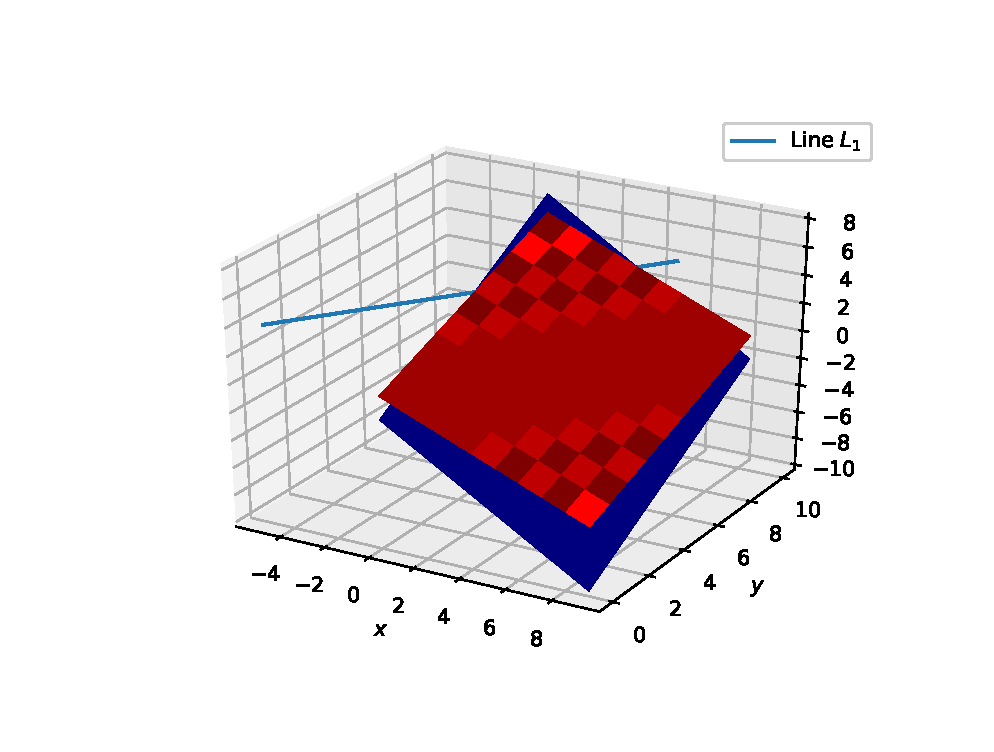
\includegraphics[width=\columnwidth]{./3d/figs/1.1.eps}
\caption{}
\label{fig:1.1}
\end{figure}

\item $L_2$ is the intersection of the planes
\begin{align}
\myvec{1 & 2 & -1}\vec{x} &= 3
\\
\myvec{3 & -1 & 2}\vec{x} &= 1
\end{align}
Show that its equation is
%
\begin{align}
\vec{x} = \frac{1}{7}\myvec{ 5 \\ 8 \\ 0} + \lambda_2 \myvec{ -3 \\ 5 \\ 7}
\label{eq:l2}
\end{align}
\item Plot 
$L_2$.
\\
\solution The following code generates Fig. \ref{fig:1.2}.
\begin{lstlisting}
 
codes/3d/1.2.py
\end{lstlisting}
\begin{figure}[!ht]
\centering
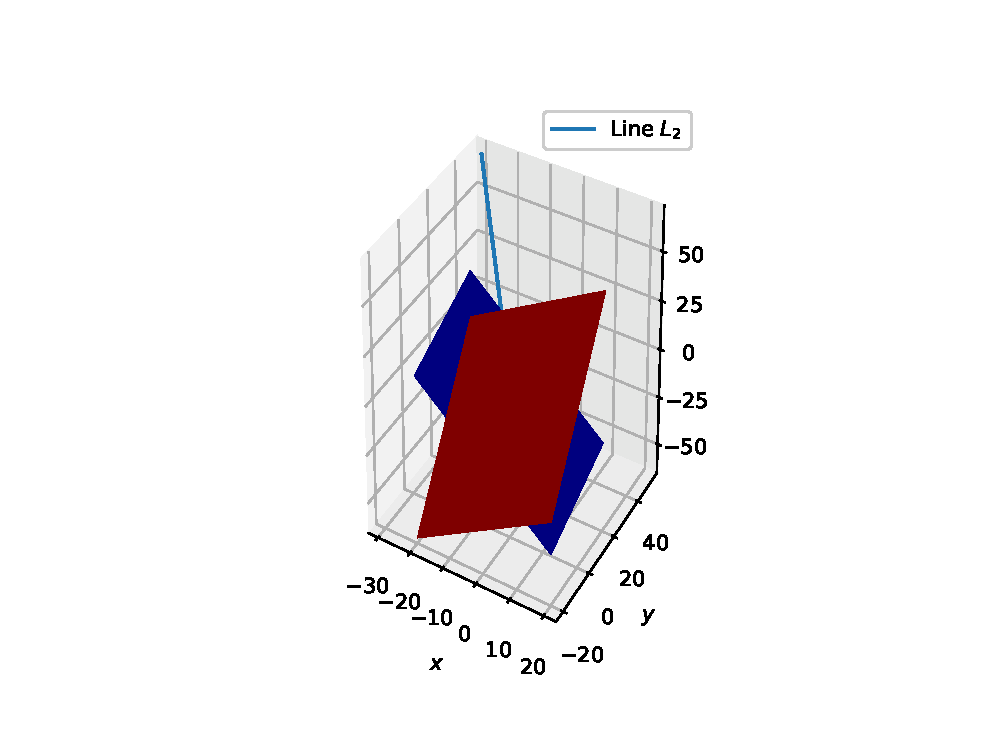
\includegraphics[width=\columnwidth]{./3d/figs/1.2.eps}
\caption{}
\label{fig:1.2}
\end{figure}

\item Do $L_1$ and $L_2$ intersect? If so, find their point of intersection $P$.
\\
\solution From \eqref{eq:l1},\eqref{eq:l2}, the point of intersection is given by
\begin{align}
\label{eq:l1l2pt}
\vec{x} = \frac{1}{7}\myvec{ 5 \\ 8 \\ 0} + \lambda_2 \myvec{ -3 \\ 5 \\ 7} &= \myvec{ 
-5 \\ 0 \\ 4} + \lambda_1 \myvec{ 1 \\ 1 \\ 0}
\\
\implies 
\myvec{1 &  3 \\ 1 & -5 \\ 0 & -7}\vec{\Lambda} &= \frac{1}{7}\myvec{40 \\ 8 \\ -28}
\end{align}
This matrix equation can be solved as
\begin{align}
\myvec{1 &  3 & \frac{40}{7}\\ 1 & -5 &\frac{8}{7}\\ 0 & -7 & -4} &\leftrightarrow \myvec{8 &  0 & 
\frac{224}{7}\\ 0 & 1 &\frac{4}{7}\\ 0 & 1 & \frac{4}{7} }
\\
\leftrightarrow \myvec{1 &  0 & 
4\\ 0 & 1 &\frac{4}{7} } &\implies \vec{\Lambda} = \myvec{4\\\frac{4}{7}}
\end{align}
%
Substituting $\lambda_1 = 4$ in \eqref{eq:l1l2pt}
\begin{align}
\vec{x} = \myvec{4 \\ 4 \\ 0} + \myvec{-5 \\ 0 \\ 4} = \myvec{-1\\ 4\\ 4}
\end{align}
\item Plot $P$.
\\
\solution The following code generates Fig. \ref{fig:1.3}.
\begin{lstlisting}
 
codes/3d/1.3.py
\end{lstlisting}
\begin{figure}[!ht]
\centering
\includegraphics[width=\columnwidth]{./3d/figs/1.3.eps}
\caption{}
\label{fig:1.3}
\end{figure}
\end{enumerate}
 
\subsection{Normal to a Plane}
\renewcommand{\theequation}{\theenumi}
\begin{enumerate}[label=\arabic*.,ref=\thesubsection.\theenumi]
\numberwithin{equation}{enumi}
\item The cross product of $\vec{a},\vec{b}$ is defined as
\begin{equation}
\label{eq:cross}
\vec{a}\times \vec{b} = \myvec{0 & -a_3 & a_2 \\ a_3 & 0 & -a_1 \\ -a_2 & a_1 & 0}\myvec{b_1 \\ b_2 \\ b_3}
\end{equation}
From \eqref{eq:l1}, \eqref{eq:l2}, the direction vectors of $L_1$ and $L_2$ are
\begin{equation}
\myvec{1 \\ 1 \\ 0} \text{ and } \myvec{-3 \\ 5 \\ 7}
\end{equation}
respectively. Find the direction vector of the normal to the plane spanned by $L_1$ and $L_2$.
\\
\solution The desired vector is obtained as
\begin{align}
\myvec{1 \\ 1 \\ 0} \times \myvec{-3 \\ 5 \\ 7} = 
 \myvec{0 & 0 & 1 \\ 0 & 0 & -1 \\ -1 & 1 & 0}\myvec{-3 \\ 5 \\ 7}
= \myvec{7 \\ -7 \\ 8} = \vec{n}
\end{align}
\item Summarize all the above computations through a plot 
\\
\solution The following code generates Fig. \ref{fig:2.1}.
\begin{lstlisting}
wget 
https://github.com/gadepall/school/raw/master/linalg/book/3d/codes/2.1.py
\end{lstlisting}
\begin{figure}[!ht]
\centering
\includegraphics[width=\columnwidth]{./3d/figs/2.1.eps}
\caption{}
\label{fig:2.1}
\end{figure}
\item Find the equation of the plane spanned by $L_1$ and $L_2$.
\\
\solution Let $\vec{x}_0$ be the intersection of $L_1$ and $L_2$.  Then the equation of the plane is
\begin{align}
\brak{\vec{x}-\vec{x}_0}^T\vec{n} &= 0
\\
\implies \vec{x}^T\vec{n} &= \vec{x}_0^T\vec{n}
\\
\implies \vec{x}^T\myvec{7 \\ -7 \\ 8} &= \myvec{-1 & 4 & 4}\myvec{7 \\ -7 \\ 8} =  -3
\end{align}
\item Summarize  the above through a plot. 
\\
\solution The following code generates Fig. \ref{fig:2.2}.
\begin{lstlisting}
wget 
https://github.com/gadepall/school/raw/master/linalg/book/3d/codes/2.2.py
\end{lstlisting}
\begin{figure}[!ht]
\centering
\includegraphics[width=\columnwidth]{./3d/figs/2.2.eps}
\caption{}
\label{fig:2.2}
\end{figure}
\item
Find the distance of the origin from the plane containing the lines $L_1$ and $L_2$.
\\
\solution The distance from the origin to the plane is given by
\begin{equation}
\frac{\abs{\vec{x}_0^T\vec{n}}}{\norm{n}} = \frac{1}{3\sqrt{2}}
\end{equation}
\end{enumerate}
 
\subsection{Projection on a Plane}
\renewcommand{\theequation}{\theenumi}
\begin{enumerate}[label=\arabic*.,ref=\thesubsection.\theenumi]
\item Write down the equations of the polars of the following points with regard to the circle 
\begin{align}
\norm{\vec{x}}^2=6
\end{align}

%\begin{multicols}{2}
\begin{enumerate}
\item
$
\myvec{2\\-1}
$
\item
$
\myvec{3\\4}
$
\end{enumerate}
%\end{multicols}
\item Find the poles of the following lines with regard to the circle 
\begin{align}
\norm{\vec{x}}=3
\end{align}

\begin{enumerate}
\item
$
\myvec{3 & 4}\vec{x}=7
$
\item
$
\myvec{5 & -1}\vec{x}+6=0
$
\end{enumerate}
and verify that the polar of their point of intersection is the line joining their poles.
\item Show that the points $\myvec{4\\-2}$, $\myvec{3\\-6}$ are conjugate with regard to the circle
\begin{align}
\norm{\vec{x}}^2=24
\end{align}
\item Prove that the lines 
\begin{align}
\myvec{5 & 3}\vec{x}=40
\\
\myvec{7 & -5}\vec{x}=10
\end{align}
are conjugate with regard to the circle
\begin{align}
\norm{\vec{x}}^2=20
\end{align}
\item Find the polar of the point $\myvec{5\\4}$ with regard to the circle
\begin{align}
\vec{x}^T\vec{x}-\myvec{4 & 3}\vec{x}-8 = 0
\end{align}
\item Find the pole of 
\begin{align}
\myvec{l & m}\vec{x}+n = 0
\end{align}
with regard to
\begin{enumerate}
\item
$
\norm{\vec{x}}=a
$
\item
$
\vec{x}^T\vec{x}+2\myvec{g & f}\vec{x}+c = 0
$

\end{enumerate}
\item Prove that if two lines at right angles are conjugate with regard to a circle one of them must pass through the centre.
\item Prove that, if the chords of contact of pairs of tangents to a circle from $\vec{P}$ and $\vec{Q}$ intersect in in $\vec{R}$, then the line joining $\vec{R}$ to
the centre is perpendicular to $PQ$.
\end{enumerate}
 
\subsection{Coplanar vectors}
\renewcommand{\theequation}{\theenumi}
\begin{enumerate}[label=\arabic*.,ref=\thesubsection.\theenumi]
\numberwithin{equation}{enumi}
\item If $\vec{u}, \vec{A}, \vec{B}$ are coplanar, show that
\begin{equation}
\vec{u}^T\brak{\vec{A}\times \vec{B}} = 0
\label{eq:coplanar}
\end{equation}
%
\item Find $\vec{A}\times \vec{B}$ given
\begin{align}
\vec{A}=\myvec{2 & 3 & -1}^T
\\
\vec{B}=\myvec{0 & 1 & 1}^T
\end{align}
\solution From \eqref{eq:cross},
\begin{align}
\vec{A}\times \vec{B} &= \myvec{0 & 1& 3 \\ -1 & 0 & -2 \\ -3 & 2 & 0}\myvec{0 \\ 1 \\ 1}
\\
&= \myvec{4 \\ -2 \\ 2}
\label{eq:last_axb}
\end{align}

\item Let $\vec{u}$ be coplanar with $\vec{A}$
%
such that $\vec{u}\perp\vec{A}$ and
\begin{equation}
\vec{u}^T\vec{B} = 24.
\label{eq:uB}
\end{equation}
Find $\norm{\vec{u}}^2$.
\\
\solution From \eqref{eq:last_axb} and the given information,
\begin{align}
\vec{u}^T\myvec{4 & -2 & 2} &=0
\\
\vec{u}^T\myvec{2 & 3 & -1} &=0
\\
\vec{u}^T\myvec{0 & 1 & 1} &=24
\\
\implies \myvec{4 & -2 & 2
\\
2 & 3 & -1
\\
0 & 1 & 1
}\vec{u}
&= \myvec{0 \\ 0 \\ 24}
\\
\implies 
\vec{u} &= 4 \myvec{-1 \\ 2 \\ 4}
\\
\implies \norm{\vec{u}}^2 &= 336
\end{align}
\end{enumerate}
 
\subsection{Least Squares}
\renewcommand{\theequation}{\theenumi}
\begin{enumerate}[label=\arabic*.,ref=\thesubsection.\theenumi]
\item Find the locus of a point which moves so that the sum of the squares of its distances from the sides of an equilateral triangle
is constant.
\item Find the locus of a point which moves so that the sum of the squares of its distances from $n$ fixed points is constant.
\item Find the locus of a point at which two given circles
subtend equal angles.
\item A circle passes through the four points $\myvec{a\\0}$, $\myvec{b\\0}$, $\myvec{0\\c}$, $\myvec{0\\d}$.  By what relation 
are $a$, $b$, $c$, $d$ connected?  Find the equation of the 
circle and show that the tangent at the point $\myvec{a\\c+d}$ is
\begin{align}
\myvec{a-b & c+d}\vec{x}
-a\brak{a-b}-\brak{c+d}^2=0
\end{align}
\numberwithin{equation}{enumi}
\item Write down the equations of the tangents to the circles
\begin{align}
\vec{x}^T\vec{x}+\myvec{-2a & 0}\vec{x}-5 = 0
\\
\vec{x}^T\vec{x}+\myvec{0 & -2b}\vec{x}-5 = 0
\end{align}
at their points of intersection and verify that they cut at right angles.
\item Find the equation of the tangent to the circle 
\begin{align}
\norm{\vec{x}}=a
\end{align}
 at the point $\myvec{a\cos\theta\\a\sin\theta}$ and show that the length of the
tangent intercepted by the lines 
\begin{align}
\vec{x}^T\myvec{1 & 0\\0 & -1}\vec{x} = 0
\end{align}
is $\pm 2a\sec\theta$.
\item $\vec{A}$ and $\vec{B}$ are two fixed points $\myvec{c\\0}$, $\myvec{-c\\0}$, and $\vec{P}$ moves so that $PA=k.PB$.  Find the locus of $\vec{P}$ and prove that it is 
cut orthogonally by any circle through $\vec{A}$ and $\vec{B}$.
\item Show that the common chord of the circles
\begin{align}
\vec{x}^T\vec{x}-\myvec{6 & 4}\vec{x}+9 = 0
\\
\vec{x}^T\vec{x}-\myvec{8 & 6}\vec{x}+23 = 0
\end{align}
is a diameter of the latter circle and find the angle at which the circles cut.
\item Prove analytically that the tangents to a circle at the ends of a chord are equally inclined to the chord.
\item Prove that for different values of $a$ the equation
\begin{align}
\vec{x}^T\vec{x}+\myvec{-2a\text{cosec}\alpha & 0}\vec{x}+a^2\cot^2\alpha = 0
\end{align}
represents a family of circles touching the lines 
\begin{align}
\myvec{\pm\tan\alpha & 1}\vec{x} = 0
\end{align}
%
Prove also that the locus of the poles of the line 
\begin{align}
\myvec{l & m}\vec{x} = 0
\end{align}
 with regard to the circles is the line
\begin{align}
\myvec{m\sin^2\alpha & l\cos^2\alpha}\vec{x}=0
\end{align}
\item Find the coordinates of the middle point of the chord 
\begin{align}
\myvec{l & m}\vec{x} = 1
\end{align}
of the circle
\begin{align}
\vec{x}^T\vec{x}+2\myvec{g & f}\vec{x}+c = 0
\end{align}
\item Prove that the points of intersection of the line 
\begin{align}
\myvec{l & m}\vec{x} = 1
\end{align}
and the circle
\begin{align}
\vec{x}^T\vec{x}+2\myvec{g & f}\vec{x}+c = 0
\end{align}
subtend a right angle at the origin if
\begin{align}
c\brak{l^2+m^2}+2gl+2fm+2=0
\end{align}
\item Prove that the equation of the circle having for diameter the portion of the line 
\begin{align}
\myvec{\cos\alpha & \sin\alpha}\vec{x} = p
\end{align}
 intercepted by the circle 
\begin{align}
\norm{\vec{x}} = a
\end{align}
 is
\begin{align}
\vec{x}^T\vec{x}-2p\myvec{\cos\alpha & \sin\alpha}\vec{x}+2p^2-a^2 = 0
\end{align}
\item Prove that if a chord of the circle 
\begin{align}
\norm{\vec{x}} = a
\end{align}
subtends a right angle at a fixed point $\vec{x}_1$, the locus of the middle point
of the chord is
\begin{align}
2\vec{x}^T\vec{x}-2\vec{x}_1^T\vec{x}+\norm{\vec{x}_1}^2 - a^2  = 0
\end{align}
\item Prove that the equation of any tangent to the circle
\begin{align}
\norm{\vec{x}-\myvec{a\\b}} = r
\end{align}
may be written in the form
\begin{align}
\myvec{\cos\theta & \sin\theta}\brak{\vec{x}-\myvec{a\\b}} = r
\end{align}
Deduce that the equation of the tangents from $\vec{x}_1$ to the circle is
\begin{multline}
r^2\norm{\vec{x}-\vec{x}_1}^2
\\
 =\sbrak{\cbrak{\vec{x}-\myvec{a\\b}}\myvec{0 & -1\\1 & 0}\cbrak{\vec{x}_1-\myvec{a\\b}}}^2
\end{multline}
\item Prove that the distances of two points from the centre of a circle are proportional to the distance of each point from the polar of the
other.
\item Prove that the tangents to the circles of a coaxal system drawn from a limiting point are bisected by
the radical axis.
\item Show that a common tangent to the two circles is bisected by their radical axis and subtends a right angle at either limiting point.
\item Prove that if a point moves so that the difference of the squares of the tangents from it to two given circles is constant its locus
 is a straight line parallel to the radical axis of the circles.
 \item Prove that the polars of a fixed point with regard to a family of coaxal circles all pass through another fixed point.
 \item The circles
 \begin{align}
\vec{x}^T\vec{x}+\myvec{-2a\sec\alpha & 0}\vec{x}-a^2 = 0
 \\
\vec{x}^T\vec{x}+\myvec{0 & -2a\text{cosec}\alpha}\vec{x}-a^2 = 0
 \end{align}
 where $\alpha$ is a given angle, both cut orthogonally every member of a coaxal family of circles.  Find the radical axis and the limiting
 points of the family.
 \item Prove that, if two points $\vec{P}$, $\vec{Q}$ are conjugate with regard to a circle, the circle on $PQ$ as diameter cuts the first circle orthogonally. 
 \item Prove that if $\vec{P}$, $\vec{Q}$ are conjugate points with regard to a circle, the circles
 with $\vec{P}$, $\vec{Q}$ as centres which cut the given circle orthogonally are orthogonal to one another.
 \item Prove that, if $PQ$ is a diameter of a circle, then $\vec{P}$, $\vec{Q}$ are conjugate points with regard to
 any circle which cuts the given circle orthogonally.
 \item Prove that if $\vec{P}$, $\vec{Q}$ are conjugate points with regard to a circle, the square on $PQ$ is equal to the
 sum of the squares on the tangents from $\vec{P}$, $\vec{Q}$ to the circle.
\renewcommand{\theequation}{\theenumi}
 \item The equation 
 \begin{align}
\vec{x}^T\vec{x}+\myvec{-2g & 0}\vec{x}+2g-5 = 0
 \end{align}
 where $g$ is a variable parameter, represents a family of coaxial circles.  
 Show that the radius of the smallest circle of the family is 2.
 \item Prove that, if perpendiculars are drawn from a fixed point $\vec{P}$ to the polars of $\vec{P}$ with regard to a
 family of coaxial circles, then the locus of the feet of these perpendiculars is a circle whose centre
 lies on the radical axis of the family.
\numberwithin{equation}{enumi}
 \item Prove that, if the points in which the line 
 \begin{align}
\myvec{l & m}\vec{x}+n=0
 \end{align}
meets the circle, 
 \begin{align}
\vec{x}^T\vec{x}+2\myvec{g & f}\vec{x}+c = 0
 \end{align}
 and those in which the line 
 \begin{align}
\myvec{l_1 & m_1}\vec{x}+n_1=0
 \end{align}
 meets 
 \begin{align}
\vec{x}^T\vec{x}+2\myvec{g_1 & f_1}\vec{x}+c_1 = 0
 \end{align}
lie on a circle,
 then 
 \begin{multline}
 2\brak{g-g_1}\brak{mn_1-m_1n}+2\brak{f-f_1}
 \\
 \brak{nl_1-n_1l}+\brak{c-c_1}\brak{lm_1-l_1m}=0
 \end{multline}
 \item Show that, if a diameter of a circle is the portion of the line 
 \begin{align}
\myvec{l & m}\vec{x}=1
 \end{align}
intercepted by the lines 
 \begin{align}
\vec{x}^T\myvec{a & h\\h & b}\vec{x} = 0
 \end{align}
 then the 
 equation of the circle is
 \begin{multline}
\brak{am^2-2hlm+bl^2}\vec{x}^T\vec{x}
\\
+2\myvec{\brak{hm-bl} & \brak{hl-am}}\vec{x}+ a+b = 0
 \end{multline}
\item Prove that, as $k$ varies, the equation
 \begin{align}
\vec{x}^T\vec{x}+2\myvec{a & b}\vec{x}+c + 2k\cbrak{\myvec{a & -b}\vec{x}+1}= 0
 \end{align}
 represents a system of coaxial circles.  Also prove that the orthogonal system is given by
 \begin{align}
\vec{x}^T\vec{x}+\myvec{\frac{c+2}{2a} & \frac{c-2}{2b}}\vec{x}+h\cbrak{\myvec{\frac{1}{2a}&\frac{1}{2b}}\vec{x} + 1} = 0
 \end{align}
 where $h$ is a variable parameter.
\end{enumerate}
 
\subsection{Orthogonality}
\renewcommand{\theequation}{\theenumi}
\begin{enumerate}[label=\arabic*.,ref=\thesubsection.\theenumi]
\numberwithin{equation}{enumi}

\item Let
\begin{align}
L_1: \quad \vec{x} &= \myvec{1 \\ 0 \\ 0} + \lambda_1 \myvec{-1 \\ 2 \\ 2}
\\
L_2: \quad \vec{x} &=  \lambda_1 \myvec{2 \\-1 \\ 2}
\end{align}
%
Given that  $L_3 \perp L_1, L_3 \perp L_2$, find $L_3$.
\\
\solution Let 
\begin{align}
L_3: \quad \vec{x} &= \vec{c}+ \lambda \vec{m}_3
\end{align}
% 
Then
\begin{align}
\myvec{-1 & 2 & 2
\\
2 &-1 & 2}\vec{m}_3 = \vec{0}
\end{align}
%
Row reducing the coefficient matrix,
\begin{align}
\myvec{-1 & 2 & 2
\\
2 &-1 & 2} &\leftrightarrow 
\myvec{1 & -2 & -2
\\
0 &1 & 2} 
\\
\leftrightarrow 
\myvec{1 & 0 & 2
\\
0 &1 & 2} 
& \implies \vec{m}_3 = \myvec{2 \\ 2 \\ -1}
\end{align}
%
Also, $L_1\perp L_2$, but $L_1 \cup L_2 = \phi$. The given information can be summarized as
\begin{align}
\label{eq:12-given1}
L_1: \quad \vec{x} &= \vec{c}_1 + \lambda_1 \vec{m}_1
\\
L_2: \quad \vec{x} &=  \lambda_2 \vec{m}_2
\\
L_3: \quad \vec{x} &= \vec{c}_3 + \lambda \vec{m}_3
\label{eq:12-given3}
\end{align}
%
where
\begin{align}
\label{eq:12-given12}
\vec{c}_1 = \myvec{1 \\ 0 \\ 0}, \vec{m}_1=  \myvec{-1 \\ 2 \\ 2},
\vec{m}_2 = \myvec{2 \\-1 \\ 2}
\end{align}
The objective is to find $\vec{c}_3$.  Since $L_1 \cup L_3 \ne \phi, L_2 \cup L_3 \ne \phi$, from \eqref{eq:12-given1}-\eqref{eq:12-given3},
\begin{align}
\label{eq:12-isect13}
\vec{c}_1 + \lambda_1 \vec{m}_1 &= \vec{c}_3 + \lambda_3 \vec{m}_3
\\
  \lambda_2 \vec{m}_2 &= \vec{c}_3 + \lambda_4 \vec{m}_3
\label{eq:12-isect23}
\end{align}
%
Using the fact that $L_1\perp L_2\perp L_3$, \eqref{eq:12-isect13}-\eqref{eq:12-isect23} can be expressed as
\begin{align}
%\label{eq:12-isect13}
\vec{m}_1^T\vec{c}_1 + \lambda_1 \norm{\vec{m}}_1^2 &= \vec{m}_1^T\vec{c}_3 
\\
\vec{m}_2^T\vec{c}_1  &= \vec{m}_2^T\vec{c}_3 
\\
\vec{m}_3^T\vec{c}_1  &= \vec{m}_3^T\vec{c}_3 + \lambda_3 \norm{\vec{m}_3}^2
\\
0 &= \vec{m}_1^T\vec{c}_3 
\\
  \lambda_2 \norm{\vec{m}_2}^2 &= \vec{m}_2^T\vec{c}_3 
\\
0 &= \vec{m}_3^T\vec{c}_3  + \lambda_4 \norm{\vec{m}_3}^2
%\label{eq:12-isect23}
\end{align}
%
Simplifying the above, 
\begin{align}
 \lambda_1  &= -\frac{\vec{m}_1^T\vec{c}_1}{\norm{\vec{m}}_1^2} = \frac{1}{9}
\\
 \lambda_2  &= \frac{\vec{m}_2^T\vec{c}_1}{\norm{\vec{m}}_2^2} =\frac{2}{9}
\end{align}
%
Substituting in \eqref{eq:12-isect13} and \eqref{eq:12-isect23},
\begin{align}
L_3: \quad \vec{x} &= \frac{2}{9}\myvec{4 \\ 1 \\ 1} + \lambda_3\myvec{2 \\ 2 \\ -1} \text{ or}
\\
L_3: \quad \vec{x} &= \frac{2}{9}\myvec{2 \\-1 \\ 2} + \lambda_3\myvec{2 \\ 2 \\ -1}
\end{align}
%
The key concept in this question is that orthogonality of $L_1$ and $L_2$ doesnot mean that they intersect.  They are skew lines.
\end{enumerate}
%

 

\end{document}


